\documentclass[a4paper,twoside]{ctexbook}
\usepackage[xetex,colorlinks,linkcolor=blue,bookmarks]{hyperref}
\usepackage{amsfonts,amsmath,amssymb}
\usepackage{caption,tabu,longtable}
\usepackage{graphicx}
\usepackage{subfigure}
\usepackage{BUPTthesisBachelor}
\usepackage{listings}
\usepackage{cleveref}
%前面几页不需要页眉页脚
\pagestyle{empty}
\setcounter{secnumdepth}{4}
\renewcommand{\theparagraph}{(\arabic{paragraph})}
\CTEXsetup[
        number={\theparagraph},
        format={\raggedright\bfseries\songti\zihao{-4}}
        ]{paragraph}
\begin{document}
%封面
    \begin{titlepage}
	\begin{center}
		%\noindent\scalebox{0.6}{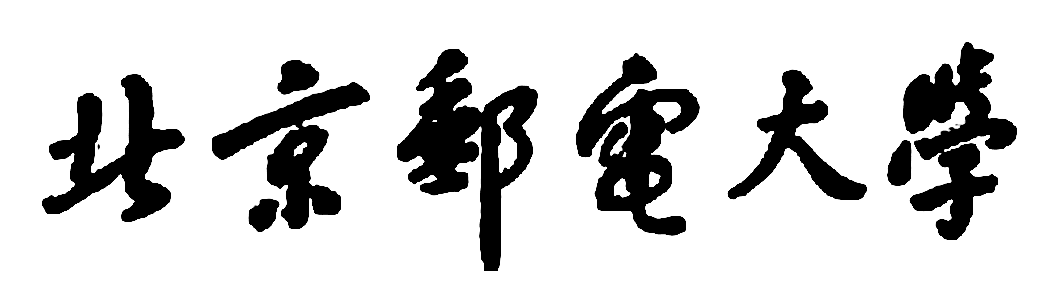
\includegraphics{figures/bupt.eps}}\\ 
		\noindent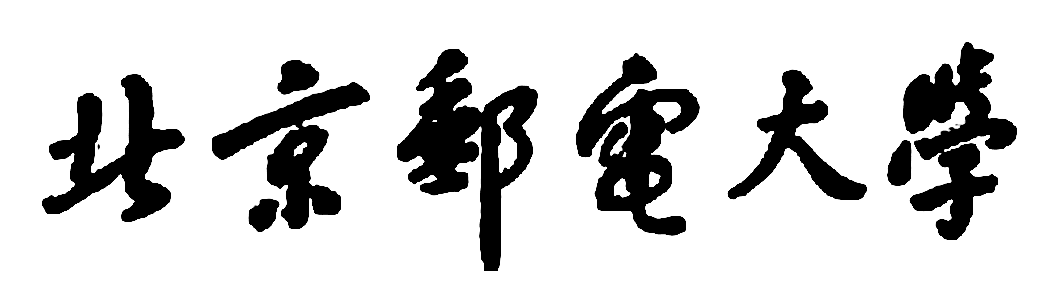
\includegraphics[height=2.5cm]{figures/bupt.eps}\\ 
		\vspace{6mm}	%本身有6.3mm的间隔
		\heiti\zihao{1}\textbf{本~科~毕~业~设~计~(论文)} \\
		\vspace{6mm}
		%\noindent\scalebox{0.25}{
\includegraphics{figures/bupt-logo.eps}}\\
		\noindent
\includegraphics[height=3.2cm]{figures/bupt-logo.eps}\\
		\vspace{2mm} %
		\setlength{\arrayrulewidth}{1pt}
		\begin{tabular}{@{}p{54.2pt}@{}p{233.4pt}}
			\heiti\zihao{3}\textbf{题目:} & \rule{0pt}{16.5pt}\zihao{3} 基于深度学习的文本情感 \\ \cline{2-2}  %这里的rule盒子起支撑作用
			\heiti\zihao{3}\mbox{~}	  & \rule{0pt}{16.5pt}\zihao{3} 分类的研究与实现 \\ \cline{2-2}
		\end{tabular}\\
		\vspace{4mm}
		\begin{tabular}{@{}p{70pt}@{}p{180pt}@{}}
			\songti\zihao{3}\textbf{姓\qquad 名} & \rule{0pt}{16pt}\songti\zihao{4}\hfill 徐心仪\hfill   \mbox{~}\\ \cline{2-2}  	%姓名
			\songti\zihao{3}\textbf{学\qquad 院} & \rule{0pt}{16pt}\songti\zihao{4}\hfill 软件学院 \hfill \mbox{~}\\ \cline{2-2}	%学院
			\songti\zihao{3}\textbf{专\qquad 业} & \rule{0pt}{16pt}\songti\zihao{4}\hfill 软件工程\hfill  \mbox{~}\\ \cline{2-2}	%专业
			\songti\zihao{3}\textbf{班\qquad 级} & \rule{0pt}{16pt}\songti\zihao{4}\hfill 2013211502 \hfill   \mbox{~}\\ \cline{2-2}  	%班级
			\songti\zihao{3}\textbf{学\qquad 号} & \rule{0pt}{16pt}\songti\zihao{4}\hfill 2013212081 \hfill     \mbox{~}\\ \cline{2-2}	%学号
			\songti\zihao{3}\textbf{班内序号} & \rule{0pt}{16pt}\songti\zihao{4}\hfill 32 \hfill     \mbox{~}\\ \cline{2-2}	%班内序号
			\songti\zihao{3}\textbf{指导教师} & \rule{0pt}{16pt}\songti\zihao{4}\hfill 吴国仕教授\hfill  \mbox{~}\\ \cline{2-2}	%指导教师
		\end{tabular}\\
		\vspace{12mm}
		%\songti\zihao{3}\textbf\today  %采用CTEX宏包自定义的时间样式,如果不喜欢可以恢复后面几行的格式
		\songti\zihao{3}\textbf{2017~年~6~月} 
%		\begin{tabular}{@{}p{56pt}@{}p{14pt}@{}p{21pt}@{}p{14pt}@{}p{28pt}@{}p{14pt}@{}}
%		\songti\zihao{4} \centering	2010&
%		\songti\zihao{4} 			年&
%		\songti\zihao{4} \centering	6&
%		\songti\zihao{4} 			月&
	%	\songti\zihao{4} \centering	17&
	%	\songti\zihao{4} 			日\\
	%	\end{tabular}
	\end{center}
\newpage
\rule{0pt}{0pt}
    \end{titlepage}


%page 诚信声明
\begin{center}
\textbf{\songti\zihao{4}\ziju{1}北京邮电大学}  
\end{center}

\begin{center}
\textbf{\songti\zihao{4}\ziju{0} 本科毕业设计(论文)诚信声明}
\end{center}
\songti\zihao{-4}

本人声明所呈交的毕业设计(论文),题目《事件相关电位(ERPs)无线同步协议设计与系统实现》是本人在指导教师的指导下,独立进行研究工作所取得的成果。尽我所知,除了文中特别加以标注和致谢中所罗列的内容以外,论文中不包含其他人已经发表或撰写过的研究成果,也不包含为获得北京邮电大学或其他教育机构的学位或证书而使用过的材料。

申请学位论文与资料若有不实之处,本人承担一切相关责任。  \newline
\indent 本人签名:\rule[-2pt]{4cm}{0.5pt}\quad 日期:\rule[-2pt]{4cm}{0.5pt}


%中文摘要
\newpage
\begin{center}
	\heiti\zihao{3}\textbf{事件相关电位(ERPs)无线同步协议设计与系统实现} 
\end{center} 
\begin{center}
	\heiti\zihao{-3}\textbf{摘\quad 要}
\end{center} 
\vspace{2.5mm}
\songti\zihao{-4}  

事件相关电位(ERPs)是与刺激信号锁定的EEG脑电信号的叠加平均。与人脑认知活动相关的事件相关电位(ERPs)成分通过模式识别的方法应用于脑-机接口,可以实现人脑与计算机的直接通信,而不依赖于外围肌肉神经系统。

事件相关电位无线同步协议及其系统实现是为基于ERP的脑-机接口系统应用提供无线连接而设计的。该协议的核心思想是子钟同步,通过在原有系统中增加一个接收无线EEG脑电数据和有线刺激事件信号的无线同步触发器完成事件相关电位所需的同步。

协议通过一个有线连接的三次握手完成通信双方的连接和同步。系统实现基于ARM内核的STM32微控制器,并兼容了无线脑电放大器原有数据帧格式。

目前系统在没有做时钟偏差校准的情况下,子钟计时累积平均误差为177us/min。该系统(无线同步触发器)在每通道字节数固定的基础上,可以自适应无线脑电放大器对于采样频率和每采样点通道数的要求。一个数据包中的刺激事件信号个数在不超过32个时不会出现丢失的情况,能远远满足一般ERPs信号无线记录的要求。每个发送到计算机的数据包的大小限制为$1024Bytes$。最后,无线同步触发器能最高接收$10KHz$采样速率的数据并提供相应精度的刺激事件信号。

\vspace{3mm}
\zihao{-4}\heiti\textbf{关键字}\quad \songti 事件相关电位 \quad 无线 \quad 脑机接口


%eAbstract
\begin{center}  
\zihao{3}\textbf{Research and Implementation of Text Sentiment Analysis Based On Deep Learning}
\end{center}
%\vspace{0.5mm}
\begin{center}  
\zihao{-3}\textbf{ABSTRACT}
\end{center}
\vspace{2mm}
\zihao{-4}

Sentiment Analysis, SA, also called Opinoin/Review Mining, is aimed at analyzing the implied status, opinion, review of the speaker. It is widely used in many fields such as public opinion analysis, automated decision support, Ads recommendation. As a subtask, Text Sentiment Classification refers to detect the sentiment polarity of the input text. Due to the rich vocabulary, semantic ambiguity, complex grammar and irregular pragmatic phenomenon of natural language, Text Sentiment Classification remains a challenging task. In this paper, we concentrate on solving Text Sentiment Classification of the sentence level with deep learning method, however, we also implement a knowledge-based algorithm for study and contrast.


To solve this problem, we build three models: first, a knowledge based model using Stanford Parser; second, to get rid of the noise from complex grammar, we discard the global grammar feature and implement an model improved from C\&W model called Convolutional Neural Network on Phrase Level(CNNPL). In the last, because CNNPL can not handle with variable length sequence, in the meanwhile, recurrent neural network   such as Long Short-Term Memory(LSTM) can not extract phrase feature, we implement a model called Convolutional Neural Network with LSTM on Phrase Level(CNNLSTMPL) which combines CNNPL and LSTM cell. Both CNNPL and CNNLSTMPL achieve good results in the task SCDL, NLPCC 2014. Their accuracies are close to or slightly exceed the best results on the contest of NLPCC 2014. 


In the meanwhile, we prompt a process for handling sentiment classification using neural network, and then we analyze the important parameters of the process. Finally, we write a website to present those model by using Restful API.

\vspace{3mm}
\zihao{-4}{\bfseries KEY WORDS}\quad Deep Learning \quad Sentiment Analysis \quad Long Short-Term Memory \quad Convolutional neural network


\frontmatter{Roman} %开始罗马页数计数
\tableofcontents
\mainmatter	%开始阿拉伯数字计页数
%从正文开始加入页眉和页脚
\pagestyle{fancy}
%正文
\chapter{绪论}

\section{研究背景及意义}
情感分析,又称为观念挖掘,指使用计算语言学的知识,对文本进行分析与自然语言处理,从而识别并抽取出语言材料中的主观信息的过程\cite{Tejwani2014}。情感分析能够自动挖掘文本信息隐含的情况,态度,意见等,在舆情分析,自动决策支持,广告推荐等方面都具有很大价值\cite{Zhang2016}。目前情感分析的主要研究领域有情感分类,情感强度预测以及观点挖掘\cite{Tejwani2014}。其中按照处理文本的粒度,情感分类任务常被划分为三种等级:一. 篇章级,也即长文本,二. 句子级,也即短文本,三. 实体或特征级,四. 单词或短语级。\cite{Zhang2016} \cite{Liu2016} \cite{Zhao2010}。实体或特征级情感分析任务具体研究语料中某个方面或者某个对象的情感,而不输出对文本整体的情感分析。本文主要关注语句级和实体级的情感分类任务,即抽取语句整体情感极性或句中实体的情感极性,判断其是否为正向,负向,中性或者矛盾。

目前国内外的研究学者和开发者主要通过三大类方法解决文本情感分类,即基于知识的方法,基于统计的方法或聚合的方法\cite{Zong2013}。基于知识的代表性算法为基于情感词典的方法,例如Kim S M等\cite{Kim2006}使用情感词典采用语义角色标注的方式衡量文本情感极性,Tong R M \cite{Tong2001}则根据不同领域使用不同的人工词典,但基于知识的方法往往实现复杂,且鲁棒性一般较差,仅能在小规模的数据上取得一定成果,很难进行进一步的优化\cite{Zong2013}。
基于统计的方法则主要为机器学习算法。由于情感分类本质上是文本分类问题,故典型的模式分类算法往往可以应用于情感分类领域,如Pang等\cite{bopang2002}采用有监督的学习方法,包括朴素贝叶斯NB,最大熵ME和支持向量机SVM,获得了比人工标注的语料库方法更好的结果。

但传统的机器学习方法如NB,ME,SVM等基本可以归类为浅层学习,这些方法难以表达复杂非线性函数,同时过度依赖于研究人员依靠经验选择的高级特征。而随着神经网络这一技术的流行,由于其可以通过神经网络中多个非线性映射的隐藏层逐层计算逼近复杂函数,同时可以自动从低级特征中学到如何表达高级特征的特性,越来越多的研究者转向使用深度神经网络进行自然语言处理,与此同时,情感分类中仍存在许多问题没有得到很好的解决,因此,本文以提高文本情感分类系统性能为目标,重点研究如何使用深度学习对文本进行情感分析。本文实现的模型具有较好的迁移性,可以运用于评论分析,舆情分析等多个领域,因此,该课题具有较高的研究价值。
\section{主要挑战}
情感分类是一个非常热门的研究领域,自提出以来经过了井喷式的发展\cite{Liu2016}。但实际分析中,待分析文本往往词汇丰富,又具有语义多样性,而且往往具有复杂的语法结构及不规范的语用现象如冗余,重复等\cite{Zong2013},并且还受到以下不可避免的问题约束,故该领域依然存在巨大挑战。
\subsection{客观语句}
定义客观语句为描述世界的客观现实的语句,而主观语句为表达个人感受,观点或信念的语句\cite{Liu2016},则在通常情况下主观语句是情感分类的主要研究对象,但实际上,主观语句可能并不带有情感信息,如“我认为蜜蜂蜇人更疼。”,而客观语句所描述的现实可能带有说话人的情感,比如“浴缸有条裂缝。”该句可能带有买家对浴缸这种商品的负向情感,故简单以主观语句作为分析对象是不行的。实际上,本文测试所用到的NLPCC 2014(The 3rd CCF Conference on Natural Language Processing \& Chinese Computing)的SCDL(Sentiment Classification with Deep Learning) 数据集,和展示用到的携程等数据集都含有大量标注为带有情感极性的客观语句。
\subsection{歧义}
歧义消解一直是自然语言处理面临的核心问题,对于“你今天怎么这么早?”这句话,根据不同的上下文语境,可能有不同的理解。如:“你今天怎么这么早?怪不得教室被打扫地这么干净。”与“你今天怎么这么早?我还没做好派对的准备。”在不同的上下文语境中,同一句话表达了不同的情感。歧义消解不仅需要考虑上下文,还往往要求系统具备某一领域的常识。在上面例子中,“没有做好派对的准备”往往代表主人还不欢迎客人的到来,也即带有负向情感。
\subsection{实体}
在系统实际处理的文本中,说话人,即输入文本的作者常与不同实体如地点,机构,人名产生联系。例如“我买了美美的家具”,该句中的“美美”可能为正向形容词,也可能为“美美家居”。当将实体词误判为形容词或相反后,语句的语法结构会被破坏,更可能引发歧义,为情感分类系统及其它自然语言处理系统带来困难。
\subsection{标注集}
由于自然语言结构复杂,故采用机器学习训练自然语言时,往往需要大量标注集作为训练语料。若采用人工方式进行标注需要大量的人力投入,实际上标注集往往通过爬取评论等带有评分的语料文本自动获取标签。但本文通过研究发现,由于不同用户的打分标准不同,采用评分方式获取标签准确度不能达到百分之百,也即训练集和测试集中往往有错误。
以下是NLPCC 2014 SCDL数据集中的一条数据,在训练集中,该句被标注为带有正面情感倾向。:
 
    <review id="225">
        不怎么怎么搞的,一带上去皮肤就过敏
    </review>
   
实际上,即使人工标注数据,也往往存在标注规范不一致的情况。
例如对于“还可以吧”这句评论,说话者既有可能带有负向情感,当说话者对比的目标都很差时,也有可能带有正向情感。
\section{研究现状}
目前情感分析领域主要采用基于知识的方法和基于统计的方法,而后者则可以分为传统浅层机器学习方法和深度学习方法,本章将分别就三种方法在句子级上的研究进展加以介绍。
\subsection{基于知识的情感分类方法}
基于知识的情感分类方法往往利用可靠的情感词典,通过分析语句中较为常见的语法关系和语法现象对语句进行情感分类。

典型的构建情感词典的方式有人工构建和自动拓展种子词的方法,而后者又分为基于知识库的方法,基于语料库的方法和二者相结合的方法\cite{Wang2016}。

基于知识库的方法一般需要有完备的语义知识库(如Wordnet)和人工事先标注正确情感的种子词,研究者依据种子词的情感极性,通过挖掘语义知识库中词语之间的关系推测未标注词的情感极性从而建立情感词典,如Hu\cite{huliu2004a}等通过同义词与反义词关系拓展情感形容词词典,最后人工筛选错误分类的词汇。由于知识库结构复杂,词汇经过若干次迭代后,可能会迭代为相反的情感极性,Kamps等\cite{Kamps04a}使用未标注词迭代为正向词和迭代为负向词所需次数之差来估计未标注词的情感极性。

由于情感词汇可能在不同的领域内表现不同的情感,因此基于知识库的方法不适用于该情景,只能构建通用情感词典,而基于语料库的方法则可以根据某领域内的大量语料推测情感词极性,能较好地解决该问题。Kanayama等\cite{Kanayama2006}认为短句中连续的情感词极性相近,遇到转折词如but后,极性则会反转。Turney\cite{turneylittman2003}使用词语与正面或负面种子词的点互信息(Pointwise mutual information, PMI)判断词语极性。二者结合的算法则能同时利用词义关系和语料中的共现信息,位置信息等关系,如Esuli\cite{Esuli2007}等使用PageRank算法,通过同义词间关系构建情感词典。深度学习在构建情感词典方面的应用也逐渐增长,如Tang\cite{Tang2014b}等改进Word2Vec模型,通过在训练时添加中心词极性和所在句子训练带有情感的短语向量(Sentiment-Specific Phrase Embedding)。

典型的使用情感词典进行情感分类的算法可能是简单将情感词加和,但更多需要结合语法特征,如Choi等\cite{Choi2008}定义一系列规则,例如对于二元词组,若第一个词为否定词,则其情感极性为第二个词的相反极性,若二者极性相同,则为该极性,否则,使用训练语料中词语的主要极性,以此计算语句极性。Moilanen等\cite{Moilanen2007}使用语法树计算语句情感极性,以此处理情感传播,极性冲突和极性转换等问题。Liang等\cite{Liang2013}则通过依赖关系进行判断。

本文实现的基于知识的情感分类模型主要基于Stanford语法树。Baker等\cite{Baker79}于1979年提出使用隐马尔科夫模型训练基于概率上下文无关文法(PCFG)的语法树。但由于PCFG将短语中的每个部分等价处理,可能导致语法二义性,Ford等\cite{Ford1982}提出了词汇化的PCFG(lexicalized-PCFG),该文法为每个规则添加规则的首要词HEAD,以获得语法树的更准确表示。Klein等\cite{Klein2003}采用标记父节点和使用马尔科夫模型决定候选规则等方式优化了未词汇化的PCFG,该方法成为了Stanford语法树的理论基础。
\subsection{基于传统机器学习的情感分类方法}
有监督算法中,Pang等\cite{bopang2002}采用有监督的学习方法,包括朴素贝叶斯NB,最大熵ME和支持向量机SVM,获得了比人工标注的语料库方法更好的结果。2004年,Pang等\cite{Pang2004}使用图最小割算法进行情感分析。Nakagawa等\cite{Nakagawa2010}使用子依存树的极性作为输入特征之一训练带有隐藏变量的CRF模型来处理情感分类问题。Mullen等\cite{Mullen2004}使用包括PMI,Osgood语法差异\cite{Osgood1957},主题相近程度和其它一些语法特征作为SVM输入。Kennedy等\cite{Kennedy2006}将转折词等也作为输入特征。Abbasi等\cite{Abbasi2008}提出了熵权重一般算法(Entropy Weighted Genetic Algorithm, EWGA)用以生成SVM的输入特征。

无监督方法中,Choi等\cite{Do2015}基于形容词在不同主题中情感极性可能不同这一特点,假设在同一主题中形容词的极性相同,提出了bootstrapping算法,该算法首先产生种子情感词,然后通过实体和情感词间的依赖关系识别训练样本中的主题将语句表达为特征向量,拓展种子词,最后通过Kmeans聚类获取语句情感分类。Lin等\cite{Lin2010}基于LDA模型实现了LSM(Latent Sentiment Model)、JST(Joint Sentiment-Topic)、Reverse-JST(Reverse-Joint Sentiment-Topic)三种无监督的情感分析模型。

半监督算法中,Davidov等\cite{Davidov2010}通过高频词和内容词等从训练语料中抽取语句模式,删除商品描述中存在的模式,将语句和模式的匹配程度作为半监督学习器的输入特征。Riloff等\cite{Riloff2003}使用Meta-Bootstrapping和Basilisk算法进行主观名词的识别并以此获取语句主客观信息。Su等\cite{Su2009}提出了半监督最小割算法。
\subsection{基于深度学习的情感分类模型}
深度学习最初使用one-hot编码表示向量,则输入特征空间复杂度至少为语句长度乘以词汇表大小,这很可能会引发维度灾难问题。Bengio等\cite{Bengio2003}根据单词上下文往往与单词自身语义有关的性质,通过训练带有一层投影层的神经网络,训练目标为用单词的上文预测单词本身来获取单词的向量表示。Mikolov等\cite{mikolov2013} \cite{mikolov2013b}改进了Bengio的算法,取消了投影层,提出了Continuous Skip-Gram模型和 Continuous Bag-of-Words模型,并使用层次softmax或负采样方法训练模型。Collobert等\cite{collobert2011}提出了C\&W模型,该模型主要分为输入层,查表层,卷积层,池化层,线性层等,被设计可应用于多种自然语言处理任务,包括对单词和语句的处理及分类,语法角色标注,词性标注等。C\&W模型也可以运用于无监督或有监督生成词向量。Tang等\cite{Tang2014c}在C\&W基础上,加入语句情感极性训练以此得到带有情感的词向量。

在使用深度学习进行情感分析方面,Socher\cite{Socher2011}使用无监督递归自编码器(RAE)预测语句语法结构与每个节点的向量表示,加入softmax层用以分类文本。但Socher认为基于单个单词的RAE无法识别短语的位置信息,而计算短语的组合函数依赖于短语中的每个单词,因此Socher在2012年\cite{Socher2012}提出了Matrix-Vector RNN模型以改进该模型。MV-RNN模型在Socher RAE模型的基础上,为每个单词添加$d \times d$了矩阵(此处d为单词表长度),用于根据上下文计算短语特征。但也正是因为该模型为每个单词添加的参数矩阵导致算法总体时空复杂度过高,需要训练的参数也过多,Socher在2013年对该模型提出了改进\cite{Socher2013},对所有节点使用一个统一的基于张量的组合函数,即为RNTN(Recursive Nerual Tensor Network)模型。Bespalov等\cite{Bespalov2011}使用滑动窗口建立n元短语表示模型并以此进行情感分析。Cao\cite{CaoXC15}结合CNN模型与SVM模型,将CNN输出作为SVM的输入特征进行训练,取得了不错的成果。
\section{论文主要研究内容及组织结构}
本文探索基于深度学习的文本情感分析方法,并针对文本情感分析的方法对模型进行改进和调整以适应特定任务。

本文主要工作内容分为以下两个部分:

1. 研究语句级的情感分析模型。本文主要实现了三个模型,基于Stanford Parser语法树的纯知识模型,基于长短时记忆循环神经网络(LSTM)的神经网络模型和基于卷积神经网络(CNN)的神经网络模型。在三个模型中CNN模型和LSTM模型在简单的评论数据集上都表现良好,但在NLPCC2014的SCDL模型上LSTM模型表现更好,在中英双语上都接近比赛评测第一名的结果,结果说明相较于CNN,RNN更适应于处理序列文本。同时,经过重复实验发现,相较于对整句抽取,对语句局部抽取特征后进行最大池化往往准确度更高,泛化能力更强。

2. 研究实体级的情感分析模型。本文通过中/英文实体识别工具为每个单词标明对应实体属性,将实体情感分类任务转化为序列到序列(seq2seq)的翻译任务。本文基于google的seq2seq模型\cite{seq2seq2014}和Attention模型\cite{attention2014}进行了改进,实现了基于LSTM和AM模型的RNN实体情感分析模型。同时,本文实现了基于CNN的实体情感分析模型作为对比。

本文组织架构如下:
\begin{itemize}
\item 第一章\ 绪论:介绍了本文的研究背景和意义,文本情感分类所面临的挑战,以及相关研究工作。同时介绍了本文的主要内容。
\item 第二章\ 数据获取与预处理:分别介绍了中英文下情感处理的一般预处理流程和流程中用到的工具。介绍了测试集及对应获取方法,以及基于stanford\ parser语法树的知识模型所用到的情感词典。
\item 第三章\ 语句级情感分析:分别介绍了基于Stanford语法树的纯知识模型,基于机器学习的CNN模型和LSTM模型的一般流程和相关知识。本章第二部分使用不同数据集对三种模型进行性能分析。最后,本章对各模型参数进行调整分析,同时提出了若干适应于文本情感分析的深度神经网络的技巧。
\item 第四章\ 实体级情感分析:介绍了实体级情感分析的一般流程,然后分别介绍了CNN模型及RNN模型和相关知识,最后使用数据集对模型进行评测,同时对参数进行分析。
\item 第五章\ 情感分析系统:本文结合各情感分析模型,实现了基于网页的评论情感分类系统。本章主要介绍系统的流程模块及实现方法。
\item 第六章\ 结束语。总结了整个研究过程中的经验,对系统的现有问题进行了归纳,对将来可以改进的地方做了总结。
\end{itemize}
\chapter{数据获取与预处理}
本章将从系统使用的数据集,情感词典和预处理流程三方面进行介绍。
\section{数据集}
为了评估数据模型的准确性以及训练模型以便展示等目的,本文针对语句级和情感级两个任务获取了以下数据集。
\subsection{语句级数据集}
\begin{center}
\begin{longtabu} to 0.8\textwidth{X|X[3]}
\hline
名称 & 手机评论数据集\\
\hline
数据总数 & 2700条\\
语言 & 中文\\
比例 & 正向:负向=1700:1000\\
词数最大值 & 300词数量级\\
90\%词数 & 50词数量级\\
情感分类准确度 & 较为正确\\
语句特点 & 语句较为规范,感情较为强烈\\
获取方式 & 实验室内部资源\\
主要用途 & 初期评估模型可行性及模型展示\\
词频统计 & 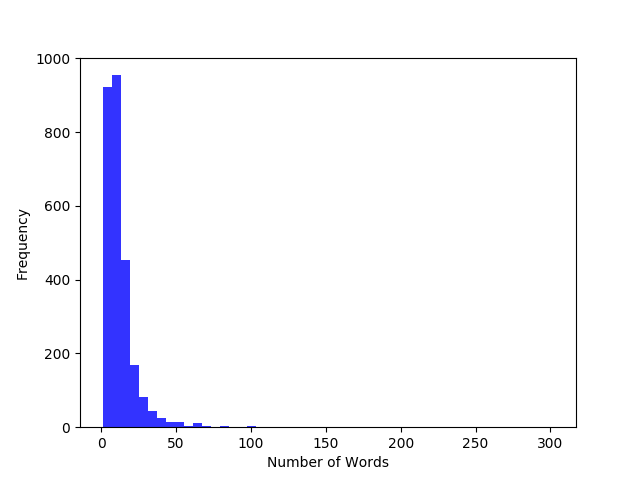
\includegraphics[width=0.6\textwidth, height=0.3\textwidth]{graphic/wordsnum_mobile.png}\\
\hline
%\caption{Mobile Dataset Word Number}
名称 & NLPCC 2014 SCDL数据集\\
\hline
数据总数 & 中文12500条,英文12485条,共24985条\\
官方测试集数据总数 & 中文2500条,英文2500条\\
语言 & 中文,英文\\
比例 & 中文 正向:负向=1700:1000\\
测试集比例 & 中文 正向:负向=1250:1250 英文 正向:负向=1250:1250\\
词数最大值 & 1000词数量级\\
90\%词数 & 200词数量级\\
情感分类准确度 & 不够准确\\
语句特点 & 语句较为口语化,有广告等中性语句\\
获取方式 & \url{http://tcci.ccf.org.cn/conference/2014/pages/page04_sam.html}(Accessed at: 5/21/2017)\\
主要用途 & 评估模型性能\\
词频统计 & 
中文\newline
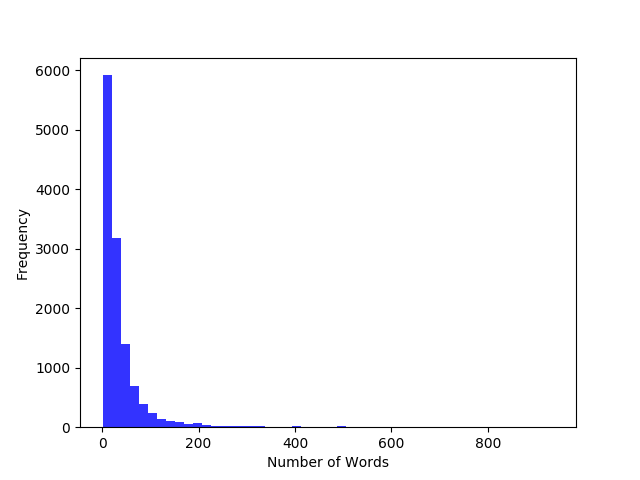
\includegraphics[width=0.6\textwidth, height=0.3\textwidth]{graphic/wordsnum_nlpcc_zh.png}
英文
\newline
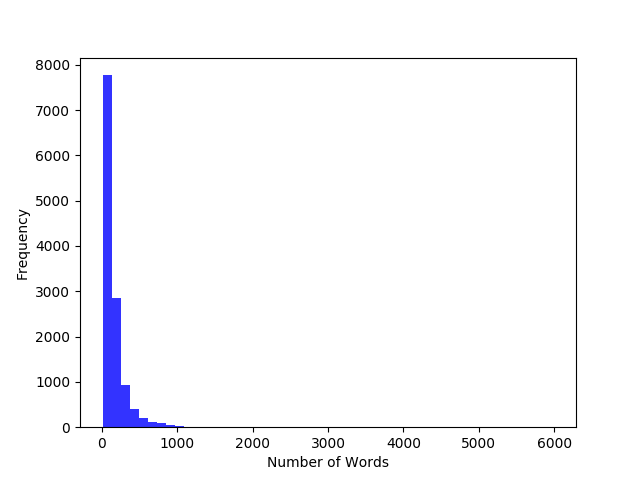
\includegraphics[width=0.6\textwidth, height=0.3\textwidth]{graphic/wordsnum_nlpcc_en.png}\\
\hline
名称 & 携程数据集\\
\hline
数据总数 & 250463条\\
语言 & 中文\\
比例 & 正向:负向=193138:57325\\
词数最大值 & 1750词数量级\\
90\%词数 & 250词数量级\\
情感分类准确度 & 不够准确\\
语句特点 & 语句较为口语化\\
获取方式 & 通过selenium模拟浏览器爬取到388067条带评分的携程酒店评论,其中评分小于4.0的定为负向,评分等于5的定为正向\\
主要用途 & 模型展示及标注实体数据集\\
词频统计 & 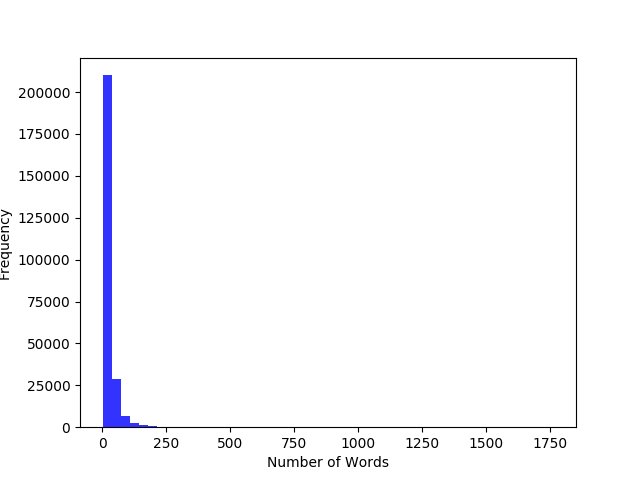
\includegraphics[width=0.6\textwidth, height=0.3\textwidth]{graphic/wordsnum_xiecheng.png}\\
\hline
\end{longtabu}
\end{center}  
\subsection{实体级数据集}
\begin{center}  
\begin{longtabu} to 0.8\textwidth{X|X[3]} 

\hline
名称 & SemEval2014Task4数据集\\
\hline
数据总数 & Laptop子数据集为3045条,Restaurants子数据集为3041条\\
语言 & 英文\\
词数最大值 & 80词数量级\\
90\%词数 & 50词数量级\\
情感分类准确度 & 较为正确\\
语句特点 & 语句较为规范,感情较为强烈\\
获取方式 & \url{http://alt.qcri.org/semeval2014/task4/}(Accessed at: 5/21/2017),取其中已标注的训练数据部分\\
主要用途 & 评估模型可行性及模型展示\\
词频统计 & 
Laptop\newline
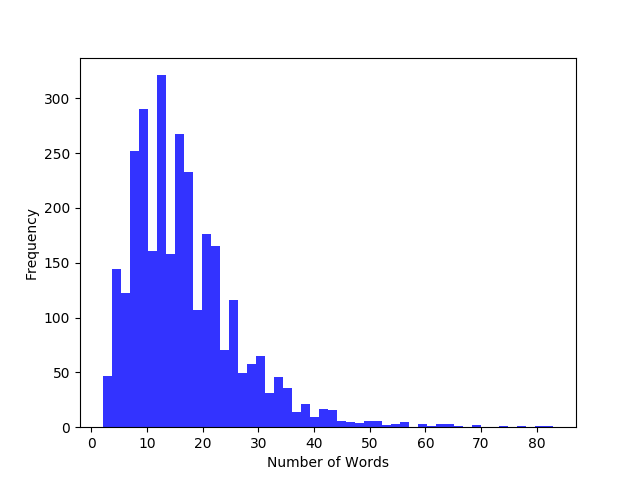
\includegraphics[width=0.6\textwidth, height=0.3\textwidth]{graphic/wordsnum_semval14_laptop.png}
\newline
Restaurant
\newline
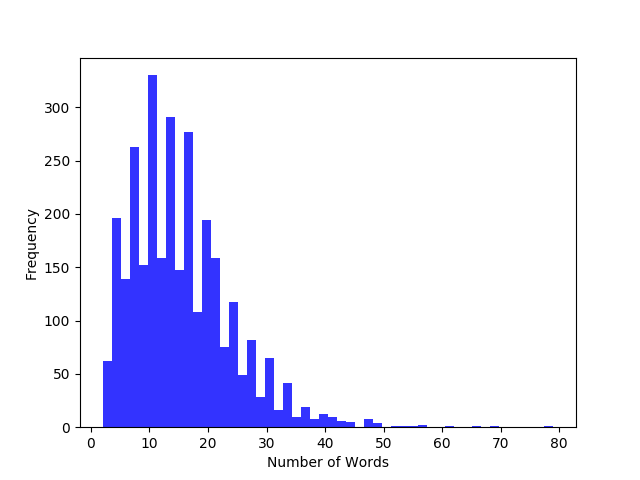
\includegraphics[width=0.6\textwidth, height=0.3\textwidth]{graphic/wordsnum_semval14_restaurants.png}\\
\\
\hline
名称 & 携程实体数据集\\
\hline
数据总数 & 6947条\\
语言 & 中文\\
词数最大值 & 100词数量级\\
90\%词数 & 20词数量级\\
情感分类准确度 & 较为正确\\
语句特点 & 语句较为规范,感情较为强烈\\
获取方式 & 对携程数据集进行过滤,取长度为10-100词之间,名词类词语只能为特定实体的语句进行手工标注实体和实体极性得到\\
主要用途 & 评估模型可行性及模型展示\\
词频统计 & 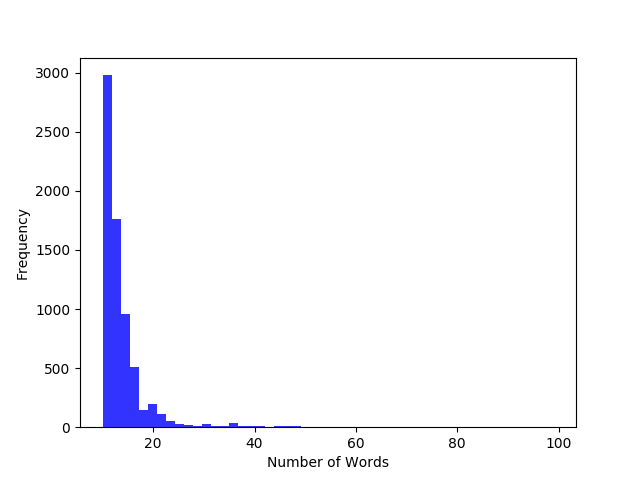
\includegraphics[width=0.6\textwidth, height=0.3\textwidth]{graphic/wordsnum_xiechengABSA.png}\\
\hline
\end{longtabu}  
\end{center}  

携程实体数据集所用到的实体如下:
\begin{itemize}
\item 地铁,整体,态度,服务员,性价比
\item 价格,前台,早餐,交通,位置
\item 设施,环境,房间,酒店
\end{itemize}
该实体集合是通过统计携程数据集上出现频率为前20的名词,经过人工筛选不规范的词汇后得到的。

\section{情感词典}
由于知识模型可以同时支持中/英文分析,故情感词典主要由以下两种语言共六个词典组成。
\subsection{中文情感词典}
\begin{enumerate}
\item Hownet(知网)情感词典\cite{hownet}:语言为中英双语,但本文主要使用中文部分。该词典为董振东和董强建立的情感分析用语集,包括主张词语,正面/负面情感词语,正面/负面评价词语,程度级别词语,并为程度级别词语划分强度等级,但其中有一些不符合构词法的词语,如“噲”,“媢”,“媢嫉”,“忺”,“安”,“巴”等在正面情感词典中出现的词。另外词语可能以短语形式出现,如“越...越...”,“abandon oneself to despaire”等。
\item NTUSD台湾大学情感词典:台湾大学自然语言处理实验室提供的情感词典,包括正面词汇2810个和负面词汇8276个,极性划分较为准确,且包含各种词性,如“一下子爆发”,“一下子爆发的一连串,“一巴掌”。
\item DUTIR情感词汇本体库:大连理工大学信息检索研究室整理和标注的中文情感词库,具有词性,情感分类,强度,极性和辅助情感分类,强度,极性等特征,划分详细。包含各种词性,但以成语和俗语为主体。
\end{enumerate}
\subsection{英文情感词典}
\begin{enumerate}
\item SentiWordNet\cite{sentiwordnet} \cite{sentiwordnet3}:基于WordNet3.0,具有语义,正向评分PosScore和负向评分NegScore等信息,本文中取PosScore-NegScore之差作为其分数。
\item Opinion Lexicon:Bing Liu等\cite{huliu2004a} \cite{huliu05a} 整理的极性情感词典,仅包含单词本身,不包含短语,但包括单词的各种变形形式。
\item 匹兹堡大学MPQA主观性词典\cite{mpqa}:是MPQA(Multi-Perspective Question Answering,多方面问答)系统所用到的词典,具有情绪词,词性,情感强弱等词汇信息。
\end{enumerate}

\section{数据预处理}
在有监督学习的过程中,如何选择特征,选择何种特征将对训练结果和泛化性产生极大的影响。实际环境中,文本往往含有不规范的表达方式及符号,需要对文本进行一系列处理。本文根据现有文献的经验,分析目前流行的文本预处理工具后,得出了下列文本预处理的流程。本文根据不同语言选择不同文本预处理工具,最终将中文或英文文本转化为可供模型分析的输入特征。

\subsection{基本流程}
如图\ref{preprocessing} 表示了整个文本情感分类系统的预处理流程,对所有模型,都需要对文本进行转换编码,去除非法字符,化繁为简和短句切分,分词这些预处理工作。其中分词则是重中之重,会对所有模型的准确率产生很大影响。对于机器模型,训练模式下需要生成词汇表,训练待编码特征对应的编码,并将语句各特征抽取出来以备训练或预测情感极性使用。
\begin{figure}[!hbp]
\begin{center}
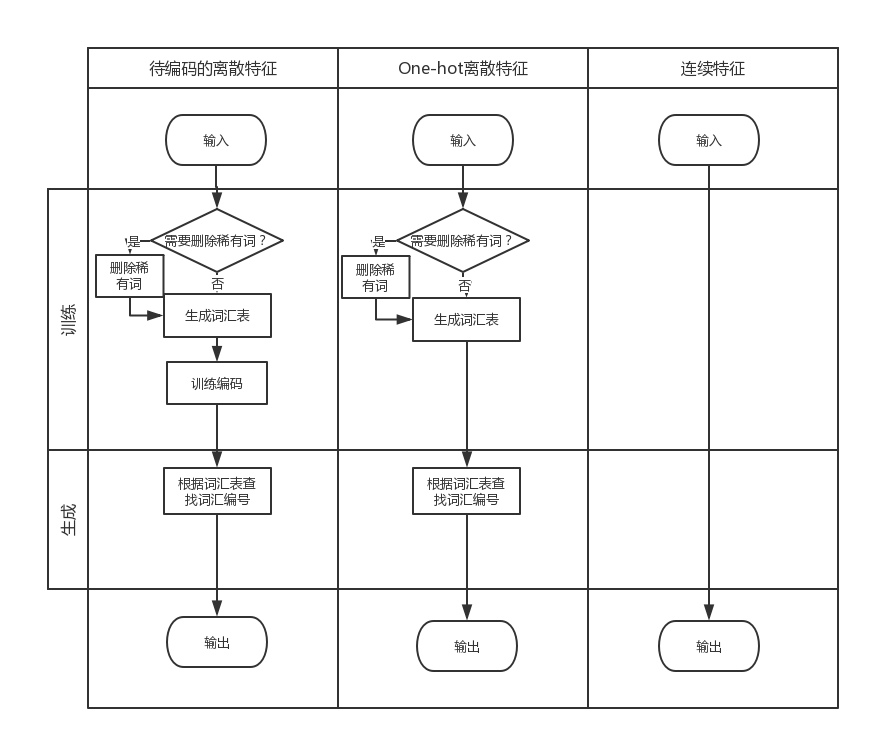
\includegraphics[width=\textwidth]{graphic/prepocessing.png}
\caption{数据预处理基本流程图 \label{preprocessing}}
\end{center}
\end{figure}

\subsection{分词和命名实体识别工具}
\subsubsection{中文}
本文分别从携程数据集,手机数据集和NLPCC中文任务中各随机抽取5条语句,使用相同的用户自定义词典,对比了三种分词工具:thulac,ansj,jieba的精准分词性能,结果如\nameref{appendix:parsercompare}所示。由于ansj工具的实体识别能力最强,故选择ansj工具。
ansj是由孙健实现的,具有分词,标注词性,实体识别,关键词抽取及新词发现功能的java中文分词工具。该工具使用隐马尔科夫模型进行语义消歧,使用Hash和高度优化Trie树进行词典匹配,并使用条件随机场模型(CRF)进行新词发现。\cite{ansjwiki} 本文主要使用到其分词,标注词性,实体识别及新词发现功能。\\
对于新词发现功能,本文主要学习输入语料中的新词,然后对这些新词进行手工过滤,加入情感词典以及ansj用户自定义词典。其中用户自定义词典人工过滤8430条,过滤得到3137条词条,157条情感词典词条。\\
\subsubsection{英文}
与没有分隔符的中文相比,英文短句中的单词之间由空格作为分隔符,更易于分隔,因而英文的分词难度远远小于中文分词。但由于英文文本中存在标点符号和不规则语用现象,本文选择使用Stanford CoreNLP工具进行分词。同时,这一步也是为了知识模型生成语法树做准备。\par
Stanford CoreNLP工具是由斯坦福大学自然语言处理实验室研发的\cite{corenlp},可以处理分句(ssplit),分词(tokenize),词性标注(POS),词干化(lemma),命名实体分析(NER),语法树分析(parse),短句情感分析(sentiment)和词语分析(natlog)等多种任务的工具集。本文中主要用到其中的分词,分句,词性标注,词干化,命名实体分析,语法树分析等功能。\par
该工具集基于Java,由管道(Pipeline)将各子工具连接,从而方便地复用了各子工具。\par
以下代码为本文系统JAVA部分调用Stanford CoreNLP工具的代码:\par
\lstset{language=java}
\begin{lstlisting}
new StanfordCoreNLP(
  PropertiesUtils.asProperties("annotators",
    "tokenize,ssplit,truecase,pos," + 
    "lemma,ner,parse,sentiment",
    "tokenize.language", "en"));
\end{lstlisting}

图\ref{fig:corenlpf1} \cite{corenlp} 是Stanford CoreNLP 整体流程的说明,如图,文本被转化为Annotation对象然后输入各子工具集,各子工具集可选,但内部存在依赖顺序。\par
表\ref{fig:corenlpf2} \cite{corenlp} 则是Stanford CoreNLP2014年各子工具集的语言支持情况,可以看到,该工具集可以处理多种语言,其中对英文支持最为全面准确。同时,该工具集支持中文的句法分析,满足知识模型需求。
\begin{center}
\begin{figure}
\subfigure[Stanford CoreNLP整体流程图]{
	\label{fig:corenlpf1}
	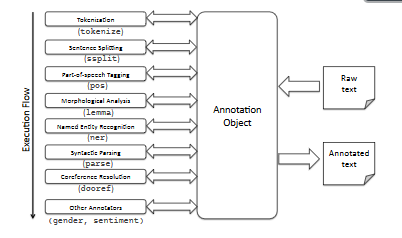
\includegraphics[width=0.4\textwidth]{graphic/stanfordcorenlpf1.PNG}
}
\subfigure[Stanford CoreNLP语言支持情况]{
	\label{fig:corenlpf2}
	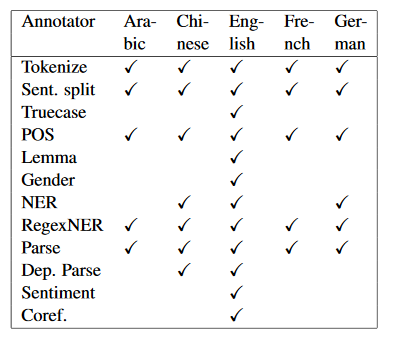
\includegraphics[width=0.4\textwidth]{graphic/stanfordcorenlpf2.PNG}
}
\end{figure}
\end{center}

\subsection{输入特征}
为了便于拓展模型和系统,本文将特征分为三类:
\begin{enumerate}
\item 待编码的离散特征,为了便于表示,称为Emb Feature。
\item One-hot离散特征: Onehot Feature。
\item 连续特征: D Feature。
\end{enumerate}
\par
三种特征各自有不同的处理方式。同时,对于某些离散特征,本文会删除词频较低的词汇,以提高模型拓展性,详细分析请见第三章。
\subsubsection{特征处理}
数据预处理方式见图\ref{featureprocessing},其中One-hot特征和Emb特征都需要转为编号,Emb特征需要进一步训练并转化为编码,生成阶段将Emb特征编号转化为编码与训练模型具体处理方式有关,因此本系统不将之列入预处理流程。
\begin{figure}[!hbp]
\begin{center}
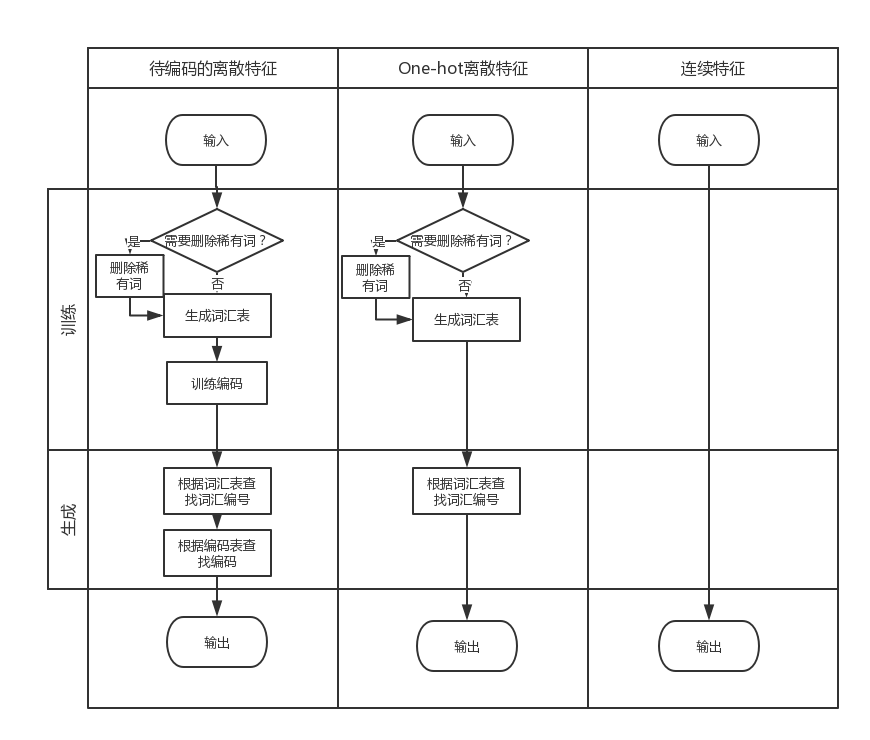
\includegraphics[width=\textwidth]{graphic/featurepocessing.png}
\caption{数据预处理基本流程图 \label{featureprocessing}}
\end{center}
\end{figure}
\subsubsection{特征选择}
\begin{center}
\begin{tabu}to \textwidth{X|X|X[3]|X[3]} 
\hline
& 层级 & 中文 & 英文\\
\hline
知识模型 & 语句级 & 词汇(D) & 词干化词汇(D)\\
\hline
CNN模型 & 语句级 & 词汇编号(Emb) & 词汇编号(Emb),词干编号(Emb)\\
\hline
RNN模型 & 语句级 & 词汇编号(Emb) & 词汇编号(Emb),词干编号(Emb)\\
\hline
CNN模型 & 实体级 & 词汇编号(Emb),词性编号(Onehot) & 词汇编号(Emb),词干编号(Emb),NER特征编号(Onehot)\\
\hline
RNN模型 & 实体级 & 词汇编号(Emb),词性编号(Onehot) & 词汇编号(Emb),词干编号(Emb),NER特征编号(Onehot)\\
\hline
\end{tabu}
\end{center}

\subsection{稀有词删除}
该步骤统计某特征的词频,对于词频小于规定次数的特征,将其置换为一个特殊词"RAREWORD"。对于词性为nt(机构团体), ns(地名), nr(人名), nz(其它专有名词)的单词所对应的特征,规定次数通常大于全局规定次数,以删除专有名词,尽量减少这类无用词的影响。

\subsection{英文词性还原及词干化}
英文中动词往往具有多种时态,如过去式,现在进行时,一般现在时等,如got,gotten,get,getting,gets。同时,形容词和副词也常常具有同样的词干,如happy, happily。这些单词虽然形态不同,却具有语义上的联系,因此,有必要对单词进行词性还原和词干提取,以发现其内部隐含的语义联系。\par
本文使用Stanford CoreNLP对单词进行词性还原,之后再使用nltk Snowball Stemmer进行词干化,以此作为英文模型的输入特征。相关测试见\nameref{appendix:lemmacompare}。
%\chapter{基于知识的情感分析模型}
基于Stanford Parser的知识模型主要使用语法特征和情感词典对文本进行情感分类,该方法不需要训练,处理短文本时速度较快,适合处理情感较为强烈,使用情感词较多,逻辑较为简单的语句。
\section{Stanford 语法树}
Stanford Parser是由斯坦福自然语言处理小组实现的语法分析工具,也是Stanford CoreNLP的其中一个组件。它主要基于概率上下文无关文法(Probabilistic Context Free Grammar,PCFG,又称随机上下文无关文法,Stochastic Context Free Grammar,SCFG),能进行句法分析和语义依存分析(Semantic Dependency Parsing, SDP),生成语法树和依赖关系,是目前比较主流的一款语法分析工具。\par
本文选择Stanford Parser作为句法分析器,因此在此简单介绍Stanford Parser的中心算法思想。\par

定义:一个概率上下文无关文法是一个五元组($N,\Sigma ,S,R,P$),其中$N$为非终结符集,$\Sigma$为终结符集,$S\in N$为开始符集,$R$为产生式集,对于任意产生式$r \in R$,其概率为$P(r)$。规则表示形式为:$A\rightarrow\alpha$,其中$A$为非终结符,$p$为$A$推导出$\alpha$的概率,即$p = P(A\rightarrow\alpha)$,该概率分布必须满足如下条件:$\sum{P(A\rightarrow\alpha)}=1$
\cite{Cha93}\par
对应于语法树,$N$相当于非叶节点,$\Sigma$为叶节点,$S$唯一且$S$为根节点,$R$为可行的路径,$P$为使用某条路径转移的概率。\par
在实践中,$P(A\rightarrow\alpha)$一般设为训练集语料中$A\rightarrow\alpha$的最大似然估计,也即$P(A\rightarrow\alpha) = \frac{Count(A\rightarrow\alpha)}{Count(A)}$,其中$Count(A\rightarrow\alpha)$为已标注语料中出现该规则的次数,$Count(A)$为语料中出现该语法单元的次数。给定语法树后,就能计算出已标注词性的文本符合语法树的概率,而寻找对应的语法树可以转化为动态规划问题求解。\par
明显,PCFG是CFG(上下文无关算法)的拓展,但上下文算法不含概率,无法解决语言的二义性问题,因此PCFG要比CFG更适合于自然语言处理。\par
但由于PCFG等价地对待词组中的所有词,导致相同结构的PCFG对词汇信息和结构偏向不明显。词汇化的PCFG文法为每个语法树的每个节点添加首要词(HEAD),从而克服了PCFG文法的弱点,取得了巨大的成功\cite{Klein2003b}。\par
本文使用Factor模型,在Stanford Parser Factor模型中词汇化的PCFG方法用于同时表示语法结构与依赖关系,如图\ref{parser1}c。Klien等\cite{Klein2003a} 人认为,设$L$为词汇化的PCFG树,则$L$可以被一棵语法PCFG树$T$(如图\ref{parser1}a)和一棵结构相符合的依赖关系树$D$(如图\ref{parser1}b)确定。于是,基于文本构建$L$的问题就被转化为基于文本构建一对$T$,$D$,使$P'(T,D)$最大,这里$P'(T,D)$代表文本同时符合$T$,$D$的概率。Klein等人进一步假设$T$与$D$相对独立,也即$P'(T,D) = P'(T)P'(D)$,并分别使用动态规划构建概率最大的$T$,$D$,之后使用A*启发式算法搜索T和D的近似结合方式,该算法取得了不错的成果。\par
Stanford Parser还对分析器做了一系列优化\cite{LevyM03} \cite{Marneffe06} \cite{Zhang2011} \cite{ChenM14} \cite{SocherBMN13} \cite{Nivre16} \cite{SchusterM16},在此不做赘述。
\begin{figure}
\begin{center}
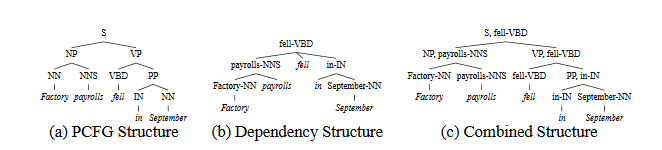
\includegraphics[width=\textwidth]{graphic/parser1.PNG}
\caption{三种分析结构 \label{parser1}}
\end{center}
\end{figure}
\section{基本流程}
算法基本流程如图\ref{plainmodel1}\par
\begin{figure}
\begin{center}
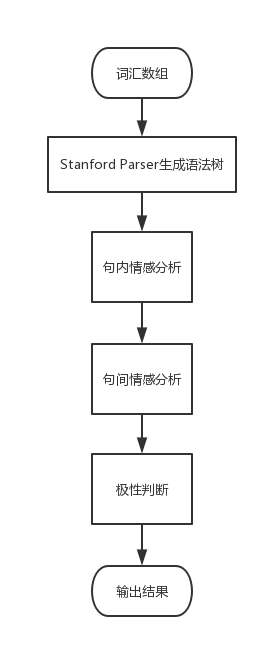
\includegraphics {graphic/plainmodel1.png}
\caption{知识模型基本流程图 \label{plainmodel1}}
\end{center}
\end{figure}
伪代码如下:\par
\lstset{language=python}
\begin{lstlisting}
def analyze(words, lang):
  if lang == 'zh':
    trees = parser_zh.parse(words)
  else:
    trees = parser_en.parse(words)
  ans = 0
  for tree in trees:
    dfs(tree.root,tree)
    ans += tree.root.sentiment
  return ans

def dfs(node, tree):
  node.phrase = ''
  if not isleaf(node):
    for child in node.daughterTrees:
      dfs(child, tree)
  if isleaf(node):
    node.phrase = node.label
  else:
      for child in node.daughterTrees:
        if lang == 'zh':
          node.phrase = node.phrase + child.phrase
        else:
          if isW(child) or child.label == "n't":
            node.phrase = node.phrase + child.phrase
          else:
            node.phrase = node.phrase + ' ' + child.phrase
  found, node.sentiment = lookup_in_emotion(node.phrase)
  if not found:
    found, node.sentiment = lookup_in_degree(node.phrase)
  if not found:
    if not isleaf(node):
      d = 0
      e = 0
      for child in daughterTrees:
        if child.label == 'RB'
          or child.label == 'AD':
          d += child.sentiment
        else:
          e += child.sentiment
      if d == 0:
        node.sentiment = e
      elif e == 0:
        node.sentiment = d
      else:
        node.sentiment = d * e
\end{lstlisting}
算法首先将分词后的词汇输入到Stanford Parser中,每个短句将生成一棵独立的语法树。\par
接着算法对每个短句所生成的语法树采用top-down递归遍历。\par
本文主要使用两个词典,一个为情感词典emotion,另一个为程度词典degree。\par
在递归的过程中,算法会首先在词典中查找子树所对应的短语,如果找到了对应的短语,则将短语所代表的情感强度或者程度强度设为该子树的强度,否则,分别统计子树的子节点的情感强度和程度强度,取其乘积作为该子树的强度。\par
最后,算法将多棵语法树根节点的情感强度相加,得到整体情感强度。\par
如图,对于“This is the right size for any use!  Uses little space and looks extremely good on the counter.”,Stanford Parser将会生成以下结果,可视化后相当于图\ref{fig:plainf2}和\ref{fig:plainf3}:\par

\begin{lstlisting}
(ROOT
  (S
    (NP (DT This))
    (VP (VBZ is)
      (NP
        (NP (DT the) (JJ right) (NN size))
        (PP (IN for)
          (NP (DT any) (NN use)))))
    (. !)))

(ROOT
  (S
    (VP
      (VP (VB Uses)
        (NP (JJ little) (NN space)))
      (CC and)
      (VP (VBZ looks)
        (ADJP (RB extremely) (JJ good))
        (PP (IN on)
          (NP (DT the) (NN counter)))))
    (. .)))
\end{lstlisting}

\begin{center}
\begin{figure}
\subfigure[语法树]{
	\label{fig:plainf2}
	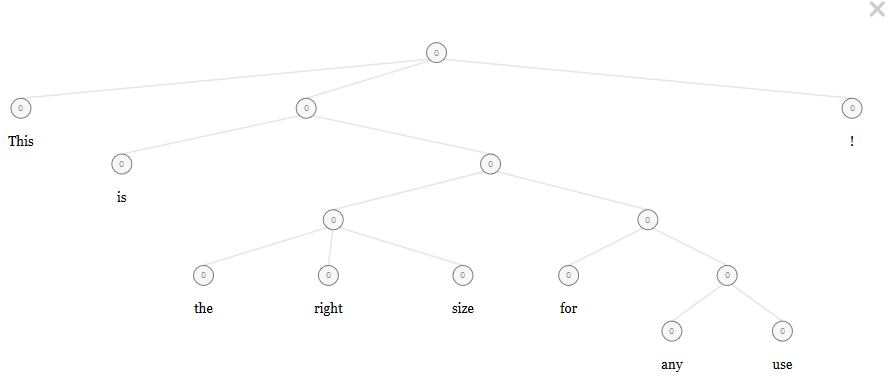
\includegraphics[width=0.8\textwidth]{graphic/plainmodel2.png}
}
\subfigure[语法树]{
	\label{fig:plainf3}
	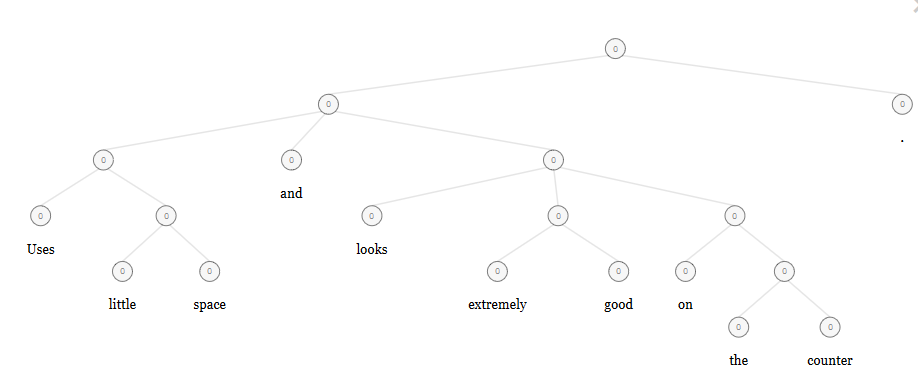
\includegraphics[width=0.8\textwidth]{graphic/plainmodel3.png}
}
\end{figure}
\end{center}

算法分别从左右两棵树根节点开始分析,逐步到达叶节点,以右边的树为例,该树对应"Uses little space and looks extremely good on the counter."。\par
\begin{enumerate}

\item 在情感词典中,"little"的情感强度为-1.0,因此"little space","Use little space"的情感强度都被标注为-1.0。
\item "extremely"在程度词典中被标注为+2.0,"good"在情感词典中被标注为+1.0,因此"extremely good", "looks extremely good on the counter."被标注为+2.0
\item 综上,"Uses little space and looks extremely good on the counter."被标注为+1.0
\item 右边的树也遵循此流程,极性为+1.0,将子句合并考虑,得到该语句整体情感强度为+2.0。
\end{enumerate}\par
最终,算法结果可视化如图\ref{fig:plainf4} \ref{fig:plainf5}。

\begin{center}
\begin{figure}
\subfigure[知识模型结果可视化]{
	\label{fig:plainf4}
	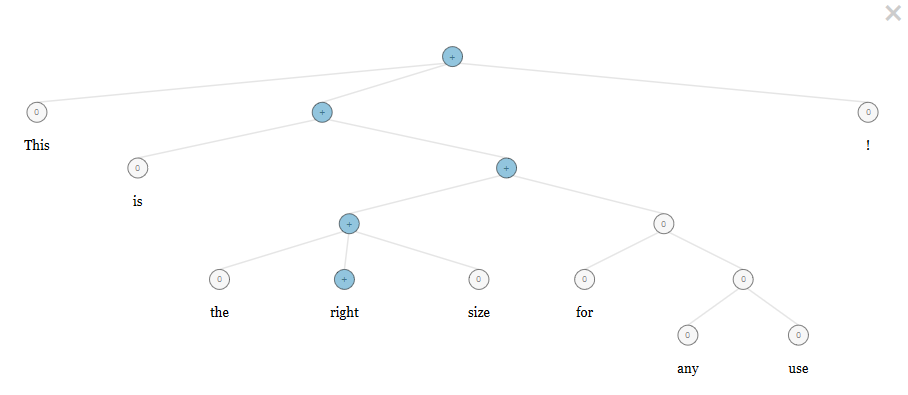
\includegraphics[width=0.8\textwidth]{graphic/plainmodel4.png}
}
\subfigure[知识模型结果可视化]{
	\label{fig:plainf5}
	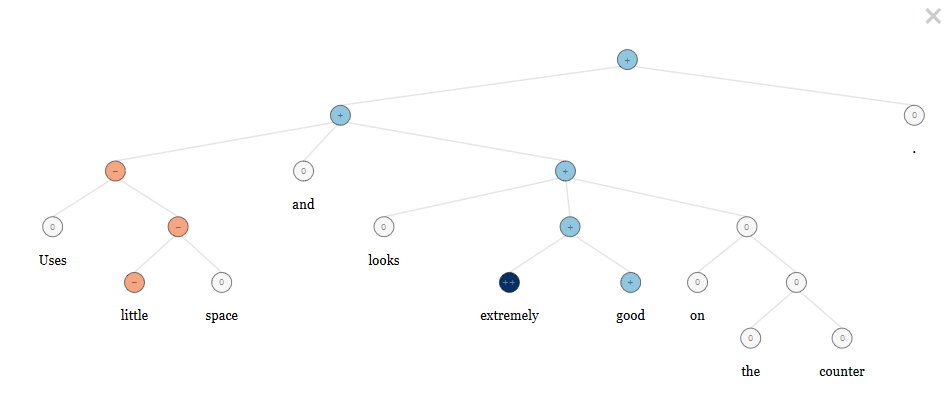
\includegraphics[width=0.8\textwidth]{graphic/plainmodel5.png}
}
\end{figure}
\end{center}

%\chapter{基于神经网络的情感分类模型}
\section{深度学习相关算法}
本节将从人工神经网络(Artificial Neural Networks, ANN)开始,分别简单介绍反向传播网络(Back Propagation, BP),卷积神经网络(Convolutional Neural Networks, CNN),循环神经网络(Recurrent Neural Networks, RNN),长短时记忆型循环神经网络(Long Short Term Memory, LSTM),优化算法等模型中可能用到的相关算法。
\subsection{人工神经网络}
人工神经网络提供了一种普遍且实用的方法从样例中学习值为实数,离散值或向量。ANN在一定程度上受到生物大脑中神经元相互连接的模型的启发,它由许多基本单元构成,每个单元有一定的实值输入(该输入可能来自外部也可能是其它单元的输出),同时产生单一的实数值输出。常见ANN的基本单元如图\ref{ann1}:
\begin{figure}[!hbp]
\begin{center}
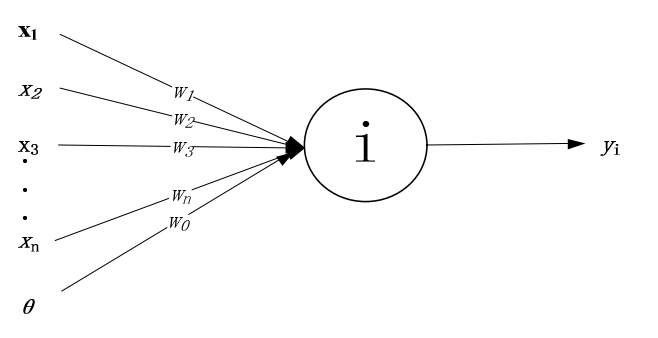
\includegraphics[width=0.4\textwidth]{graphic/ann1.png}
\caption{ANN基本单元\cite{ml2006} \label{ann1}}
\end{center}
\end{figure}
其函数可以写作
\begin{equation}
o(\vec{x}) = f(\vec{w} \vec{x} - b)
\end{equation}
其中$\vec{x}$为输入,$f$为激活函数,负责将线性输出转变为非线性输出以增加神经网络的表达能力,$\vec{w}$为权重(weights),$b$为偏置(bias),与$\vec{w} \vec{x} $具有相同形状。$\vec{w}$与$b$通常是神经网络训练的主要对象。
常用的激活函数有sigmoid(又称logistic函数),tanh,ReLu(Rectified Linear Unit)等,具体公式如下:
\begin{center}
\begin{tabu}  to 0.8\textwidth{X|X[3]|X[3]}
\hline
函数名称 & 函数 & 导数 \\
\hline
sigmoid &
$$
f(y) = \frac{1}{1 + e^{-y}}
$$
&
$$
\frac{df(y)}{dy} = f(y) \times (1 - f(y))
$$
\\ \hline
tanh &
$$
f(y) = tanh(y) = \frac{e^x - e^{-x}}{e^x + e^{-x}}
$$
&
$$
\frac{df(y)}{dy} = 1 - {f(y)}^2
$$
\\ \hline
ReLU &
$$
f(y) = \left\{\begin{matrix}
y & if\ y > 0\\ 
0 & if\ y \leq 0
\end{matrix}\right.
$$
&
$$
\frac{df(y)}{y} = \left\{\begin{matrix}
1 & if\ y > 0\\ 
0 & if\ y \leq 0
\end{matrix}\right.
$$
\\ \hline
\end{tabu}
\end{center}
由于sigmoid函数和tan函数的导数是线性输出的二次多项式,在训练时易导致梯度爆炸或梯度消失问题,故本文中线性层之间的激活函数主要选用ReLU函数。\par
一个较典型的人工神经网络通常由多层基本单元构成,如图\ref{ann2},通常有输入层,隐含层,输出层,各层之间通过激活函数将线性输出转化为非线性输出。\par

\begin{figure}[!hbp]
\begin{center}
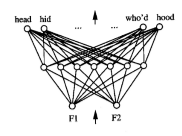
\includegraphics[width=0.4\textwidth]{graphic/ann2.png}
\caption{典型ANN结构\cite{ml2006} \label{ann2}}
\end{center}
\end{figure}

\subsection{损失计算函数}
本文中主要使用带有softmax的交叉熵函数计算网络输出值和目标值之间的误差。softmax函数是sigmoid函数在多分类问题上的拓展。
\begin{equation}
softmax(t_i) = \frac{e^{t_i}}{\sum_j{e^{t_j}}}
\end{equation}
其中$\vec{t}$为网络的输出,其长度为类别总数。
\begin{equation}
loss = crossentropy(\vec{S}, \vec{L}) 
= \sum_i {(L_i * log(s_i))}, \vec{S} = softmax{(\vec{t})}
\end{equation}
其中$\vec{L}$为网络的目标值,其长度为类别总数。

\subsection{反向传播网络}
反向传播算法是目前多层神经网络主要的训练方法,它主要基于微积分的链式求导法则\ref{chainrule},对神经网络从输出层向上进行快速求导。

\begin{equation} \label{chainrule}
(f(g(y)))' = f'(g(y)) * g'(y)
\end{equation}
反向传播神经网络的训练基本流程是:\par
\begin{enumerate}
\item 初始化网络。
\item 首先将输入沿前向传播,求出误差。
\item 使误差沿网络反向传播,计算梯度,从而使用优化方法更新权值。
\item 如果达到终止条件,跳出循环,否则,重复第2-4步。
\end{enumerate}

\subsection{优化方法}
在神经网络上训练时,其假设空间为所有可能的实数权向量的集合(将偏置等参数也视为权向量),一个高维空间。当误差函数和目标值已知时,假设空间中会形成一个误差曲面,而训练的目的就是尽可能找到该误差曲面的最小值。\par
如图\ref{ann3}是二维假设空间中误差曲面的假想图,可以看出该误差曲面是具有单一全局最小值的抛物面,沿梯度方向可以到达该最小值点。\par
\begin{figure}[!hbp]
\begin{center}
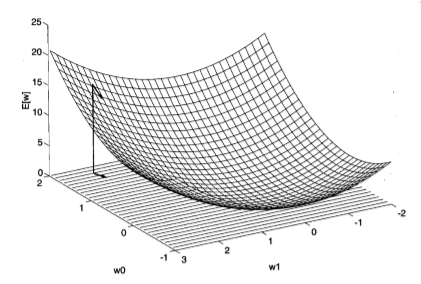
\includegraphics[width=0.4\textwidth]{graphic/ann3.png}
\caption{误差曲面\cite{ml2006} \label{ann3}}
\end{center}
\end{figure}
\subsubsection{随机梯度下降方法}
为了确定一个使误差最小化的权向量,梯度下降搜索从初始权向量出发,每一步都沿梯度方向修改该权向量,直到到达全局最小误差点。\par
该训练法则可以写为:\cite{ml2006}
\begin{equation}
w_i \leftarrow w_i + \eta\Delta w_i
\end{equation}
其中$\Delta w_i$为误差相对于分量$w_i$方向上的梯度,$\eta$为控制步长的学习速率。\par
但梯度下降方法每一步都需要计算所有训练样例上的整体误差,同时,梯度下降方法很可能收敛到局部极小值。\par
为了缓解这些困难,人们提出了随机梯度下降算法,该算法根据每个训练样例batch单独计算误差来更新权值,相当于为每个batch单独定义不同的误差函数。因此,如果误差平面上有多个局部极小值,随机梯度下降算法可以通过不同的误差避免陷入局部最小值。
\subsubsection{Adagrad方法}
虽然随机梯度下降方法为避免陷入局部最小值提供了可行的方法,但梯度下降方法对所有需要更新的权向量都使用了全局学习速率,而全局学习速率可能不适应于所有的参数。Adagrad(Adaptive Subgradient)方法\cite{adagrad}能够对每个参数自适应不同的学习速率,对稀疏特征使用更大的学习速率,因此更适应于处理稀疏数据。\par
其学习速率为:
\begin{equation}
\eta_{t, i} = \frac{\eta_0}{ \sqrt{\sum_{j=1}^{t}{G_{j,i}^2} + \epsilon}}
\end{equation}
其中,$\eta_{t, i}$为t时刻对于权重$w_i$的学习速率,$\eta_0$为初始学习速率,$\epsilon$为平滑常数,用于防止分母为0,$G_{j,i}$代表j时刻$w_i$方向上的梯度。

\subsubsection{ADADELTA方法}
Zeiler等\cite{adadelta}人认为Adagrad方法存在三个问题:
\begin{enumerate}
\item 其学习率单调递减,训练后期学习率过小。
\item 需要手工设置一个全局的初始学习率。
\item 更新$X_t$时存在单位不统一现象。
\end{enumerate}
因此Zeiler等人提出了ADADELTA方法,用于改进Adagrad方法。ADADELTA算法基于牛顿迭代法,其学习速率不再基于全部梯度平方之和,而主要基于最近的梯度。
其学习速率更新规则为:
\begin{equation}
E[g^2]_t = \rho E[g^2]_{t-1} + (1-\rho )g_t^2
\end{equation}
\begin{equation}
\eta_t =  -\frac{\sqrt{E[\eta^2]_{t-1} + \epsilon}}{\sqrt{E[g^2]_{t} + \epsilon}}g_t
\end{equation}
\begin{equation}
E[\eta^2]_t = \rho E[\eta^2]_{t-1} + (1-\rho )\eta_t^2
\end{equation}
其中$g_t$为t时刻的梯度,$\rho$为衰减速率,$\epsilon$为平滑常数。

\subsubsection{ADAM方法}
ADAM(Adaptive Moment Estimation)\cite{adam}根据损失函数对每个参数的梯度的一阶矩估计和二阶矩估计动态调整针对于每个参数的学习速率,其中一阶矩的作用类似于冲量项(momentum),二阶矩则与ADADELTA算法相似。ADAM算法迭代更新步长有一个较为稳定的范围,因此更适合RNN。

\begin{equation}
m_t = \beta_1 m_{t - 1} + (1 - \beta_1)g_t
\end{equation}
\begin{equation}
v_t = \beta_2 m_{t - 1} + (1 - \beta_2)g_t^2
\end{equation}
\begin{equation}
\hat{m_t} = \frac{m_t}{1 - \beta_1^t}
\end{equation}
\begin{equation}
\hat{v_t} = \frac{v_t}{1 - \beta_2^t}
\end{equation}
\begin{equation}
\eta_t = -\frac{\eta}{\sqrt{\hat{v_t} + \epsilon}} \hat{m_t}
\end{equation}
实践中$\beta_1=0.9$,$\beta_2=0.999$,$\epsilon = 1e-8$

\subsection{卷积神经网络}
卷积神经网络(Convolutional Neural Network, CNN)是一种前馈网络,该网络内部单元的连接模式不同于传统的全连接方式,每个神经元的输入仅与上一层对应单元核大小范围内的输出单元有关。卷积神经网络相当于在神经网络上执行卷积操作。\par
数学上的卷积函数定义如下:\par
设$x(a)$和$w(a)$为在$R$上的可导函数,则称$s(t) = \int x(a)w(t-a)da$为函数$x$与$w$的卷积,记作$s(t) = (x * w)(t)$\par
其中$x$被称为输入,$w$被称为核函数(kernel function),在统计学上,卷积操作相当于加权平均。\par
由于自然语言为离散序列,故本文使用的卷积运算核为1维,卷积公式可以写为:\par
\begin{equation}
s(t) = (x * w)(t) = \sum x(a)w(t -a)
\end{equation}
在实际使用中,a的取值范围通常较小,以减少运算,产生局部输出单元的综合输出。
下采样(downsampling)卷积函数能够每隔一段距离采样,称该距离为步长(stride),则当核为1维,核长为k时,卷积公式可以写为:
\begin{equation}
s(t) = (x * w)(t) = \sum_{i = 0}^{\lfloor{\frac{k}{stride}}\rfloor}{x(t + i \times stride)w(i \times stide)}
\end{equation}
卷积操作通过三个重要的思想帮助改进机器学习系统,即稀疏交互,参数共享和平移不变性\cite{deeplearning2016}。首先是稀疏交互,如图\ref{cnn1},传统神经网络单元会与上一层的每个输入单元产生交互,而通过限制卷积核大小,单元只会与附近的输入单元产生交互,从而大大减少了需要训练和存储的参数,提升了效率和泛化能力。然后是参数共享,在卷积神经网络中,多个位置共享同样的参数集合,而不需要针对每个位置单独训练。最后是平移不变性。如果我们在输入中移动一个事件,那么对应的输出仍会输出而且会延后相应长度。例如,对于“手机 小巧 玲珑”和“我 觉得 手机 小巧 玲珑”,当卷积核的大小为2,步长为2时,两句中的“手机 小巧”将会输出同样的结果。

\begin{figure}[!hbp]
\begin{center}
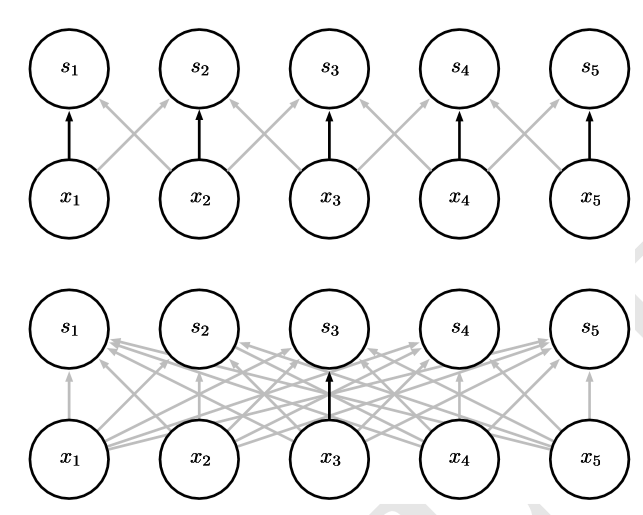
\includegraphics[width=0.4\textwidth]{graphic/cnn1.png}
\caption{CNN与ANN对比\cite{deeplearning2016} \label{cnn1}}
\end{center}
\end{figure}

\subsubsection{池化}
池化(Pooling)是卷积神经网络中非常重要的操作,能帮助学习输入特征的不变性,也能减少特征数量,增加计算速度。常见的池化方式有两种,最大池化和平均池化。最大池化给出了卷积层输出中一个矩形区域内特征的最大值,而平均池化则为矩形区域内特征的平均值。池化相当于简单使用某一位置附近区域的总体输出来代替各单元的输出。在自然语言处理中,最大池化的作用往往要好于平均池化,因此,本文采用最大池化方式。
\subsection{C\& W模型}
C\& W模型是由collobert等于2011年\cite{collobert2011} 提出的基于卷积神经网络的自然语言处理框架,该模型被设计能够适用于几乎所有自然语言处理任务,同时也能对某个任务进行细化以提高精度。C\& W模型分为两种模式,单词窗口和语句模式,后者主要结构如图\ref{candw1}。模型可以分为七层,输入层,查表层,卷积层,池化层,线性层和对应的激活函数层,最后是输出层。C\& W模型在各任务上都表现良好,接近为特定任务特化的系统性能,因此本文选择C\& W模型作为基本框架。
\begin{figure}
\begin{center}
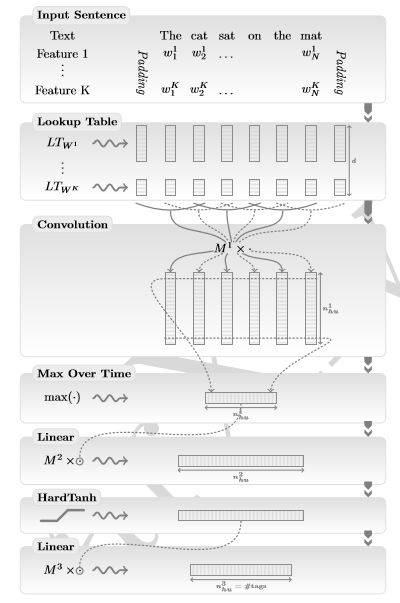
\includegraphics{graphic/candw1.png}
\caption{c\&w语句模式基本模型 \label{candw1}}
\end{center}
\end{figure}
\subsection{循环神经网络}
循环神经网络(Recurrent Neural Network)是专门用于处理序列数据的神经网络。如图,传统神经网络为序列中的每个状态分别训练权重,但RNN在时间步内共享参数。给定时间t的变量后,t+1时变量的条件概率分布是平稳的,不依赖于t,也即RNN具有时间上的平移不变性。\par
对于长度为{t}的序列$\vec{x}$,一般神经网络计算方式可以表示为:
\begin{equation}
h_t = g_t(x_t, x_{t-1},...,x_0;\theta)
\end{equation}
其中$\theta$代表所有网络参数。\par
而RNN的计算方式可以表示为:
\begin{equation}
h_t = g_t(x_t, x_{t-1},...,x_0;\theta) = f(h_{t-1}, x_t;\theta)
\end{equation}
RNN能将长度为t的序列映射为固定长度的向量,但这种映射通常是有损的,因此,需要保证$h_t$足够丰富,能够记住序列中的信息。
RNN主要有三种结构,a中每个时间步都有输出,并且隐藏单元与过去隐藏单元相关联,b中隐藏单元与过去输出相关联,而c中只有最后一个时间步有输出。由于语句级情感分析任务最终只有一个输出,所以本章中RNN结构符合c。
训练中,RNN使用通过时间反向传播算法(BPTT)反向推导t步梯度。实践中,为了降低复杂度,同时也因为梯度爆炸和梯度消失的限制,t往往取较小的定值。
\begin{center}
\begin{figure}
\subfigure{
	\label{fig:rnn1}
	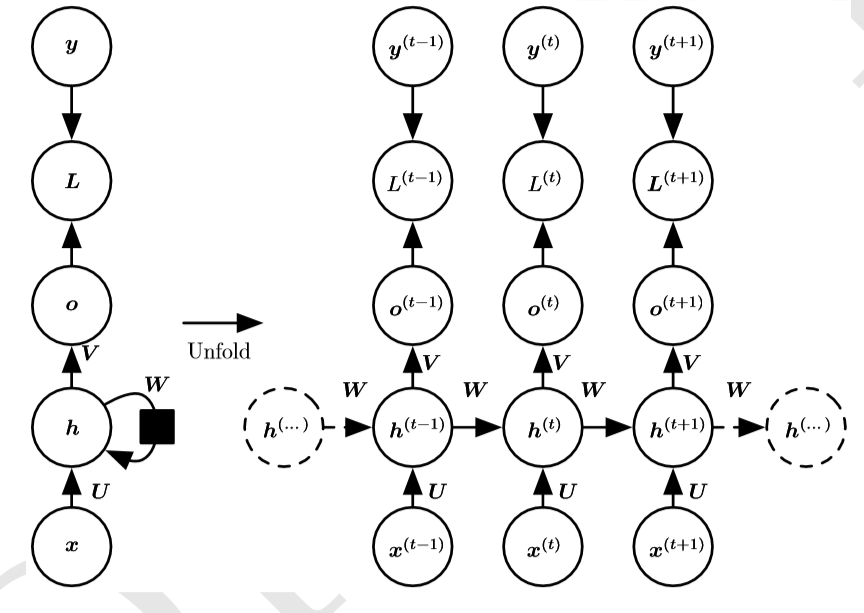
\includegraphics[width=0.3\textwidth]{graphic/rnn1.PNG}
}
\subfigure{
	\label{fig:rnn2}
	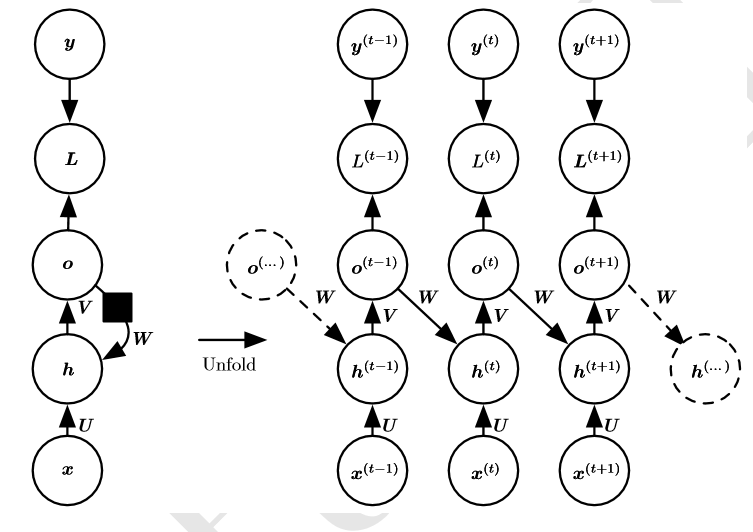
\includegraphics[width=0.3\textwidth]{graphic/rnn2.PNG}
}
\subfigure{
	\label{fig:rnn3}
	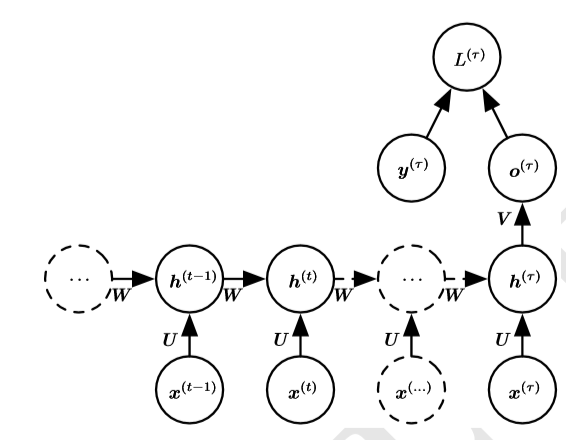
\includegraphics[width=0.3\textwidth]{graphic/rnn3.PNG}
}
\caption{RNN基本结构}
\end{figure}
\end{center}

\subsection{LSTM}
RNN为信息的持久化提供了行之有效的方法,但RNN存在梯度爆炸或梯度消失的问题。\par
考虑最简单的RNN单元,即:
\begin{equation}
h_t = W^Th_{t-1}
\end{equation}
该公式相当于:
\begin{equation}
h_t = {W^t}^Th_0
\end{equation}
若W符合下列形式的特征分解:
\begin{equation}
W=Q\Lambda Q^T
\end{equation}
则原式可以转化为:
\begin{equation}
h_t = Q^T\Lambda ^t Qh_0
\end{equation}
因此,$h_t$随时间成指数形式增长,若幅值小于1时,$h_t$将随t的增长趋向于0,出现梯度消失现象,而当幅值大于1时,$h_t$又激增,导致梯度爆炸。\par
为了减轻梯度消失问题,Hochreiter等\cite{lstm1997}提出了LSTM模型,该模型主要由以下四部分构成:
\begin{enumerate}
\item 遗忘门:控制状态更新
\item 输入门:控制信息保存。
\item 输出门:控制读取信息。
\item 记忆单元:存储状态。
\end{enumerate}
LSTM的具体计算流程如下:
\begin{equation}
i_t = \sigma(W_i  [h_{t-1},x_t] + b_i)
\end{equation}
其中$i_t$为输入门输出的结果,$W_i$为输入门的参数,$h_{t-1}$为上一时刻的输出,$x_t$为本时刻的输入,$b_i$为输入门的参数偏置。
\begin{equation}
u_t = \tanh{(W_u [h_{t-1},x_t] + b_u)}
\end{equation}
其中$u_t$为记忆单元得到的结果,$W_u$为记忆单元的参数,$b_u$为输入门的参数偏置。
\begin{equation}
f_t = \sigma{(W_f [h_{t-1},x_t] + b_f)}
\end{equation}
其中$f_t$为遗忘门输出的结果,$W_f$为遗忘门的参数,$b_f$为遗忘门的参数偏置。
\begin{equation}
C_t = f_t C_{t-1} + i_t \times u_t
\end{equation}
其中$C_t$为本时间点的状态。
\begin{equation}
o_t = \sigma{(W_o [h_{t-1},x_t] + b_o)}
\end{equation}
其中$o_t$为输出门输出的结果,$W_o$为输出门的参数,$b_o$为输出门的参数偏置。
\begin{equation}
h_t = o_t \times tanh{(C_t)}
\end{equation}
其中$h_t$为最终输出结果。
\begin{figure}[!hbp]
\begin{center}
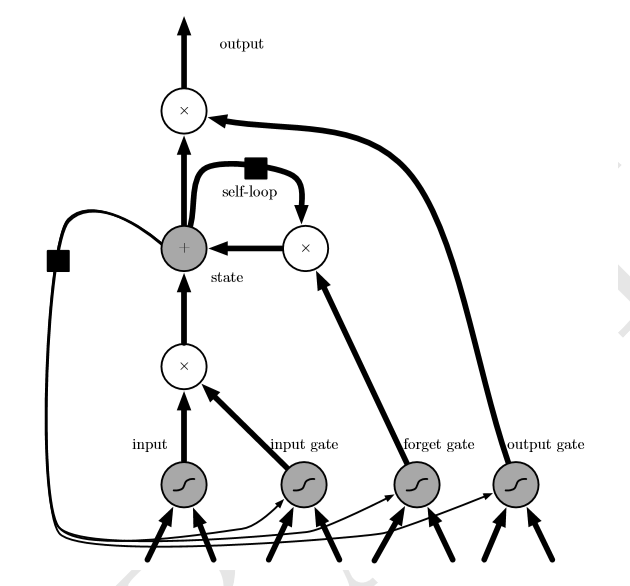
\includegraphics[width=0.4\textwidth]{graphic/lstm1.png}
\caption{LSTM基本结构\cite{deeplearning2016} \label{lstm1}}
\end{center}
\end{figure}

\section{NOLSTM模型}
本文基于C\& W模型实现了情感分类模型,由于卷积神经网络具有平移不变性,因此可以抽取出语句中短语特征,从而借此分析整体情感。
\subsection{神经网络结构}
NOLSTM模型主要分为八层,输入层,连接层,卷积层,Dropout层,三层线性层和输出层。\par
其中,如图\ref{nolstm1}输入层和连接层对应于C\& W模型的输入层和查表层,输入的离散特征在输入层转换为one-hot编码或者经过训练的编码,连接层将输入的特征包括连续特征进行连接,拓展每个词所对应的特征向量维数。输入层设计为与具体特征选择无关,以便于调整模型,也便于未来用不同的特征对模型进行拓展。\par
如图\ref{nolstm1},经过反复试验,本文中卷积层由一维五个卷积核构成,本文中取[3,5,6,7,9],不同的卷积核分别对应不同的池化层。本文中选取的池化层都为全局池化层,经过全局池化层可以提取出文本在不同长度上的全局特征。令人惊讶的是,同样经过反复试验,全局池化层的效果好于局部池化层或者堆叠局部池化层,笔者认为局部池化可以保留语句结构,而全局池化可以去除语句结构信息,而在神经网络对语句分析的过程中,过于丰富的语句结构可能反而起了抑制泛化的作用,详细参数分析见第五章。\par
Dropout层被加在卷积层之后以便于提高模型泛化性。Dropout能够随机使一些卷积层的输出失效,以迫使模型利用其它输出结果,从而尽量减少特征与某一特定输出之间的关联。\par
模型接下来使用了三层特征数目依次递减的全连接层即Linear0,Linear1,Linear2抽取高级特征,如图\ref{nolstm3},线性层之间使用ReLU函数进行激活。\par
最后模型进行误差和精度计算,并使用ADAM优化函数即图中的Optimizer进行反向传播。图中的save用于保存和读取模型。\par
由于该模型相对于特征独立,所以该模型可以被同时应用于中英双语,也可以拓展到其它语句分类任务上。

\begin{figure}[!hbp]
\begin{center}
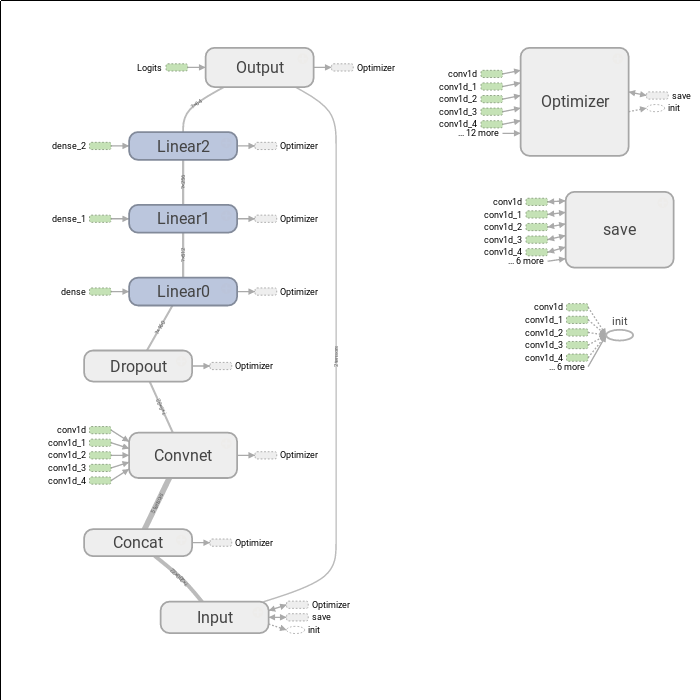
\includegraphics[width=0.8\textwidth]{graphic/nolstm1.png}
\caption{NOLSTM模型整体结构 \label{nolstm1}}
\end{center}
\end{figure}
\begin{figure}[!hbp]
\begin{center}
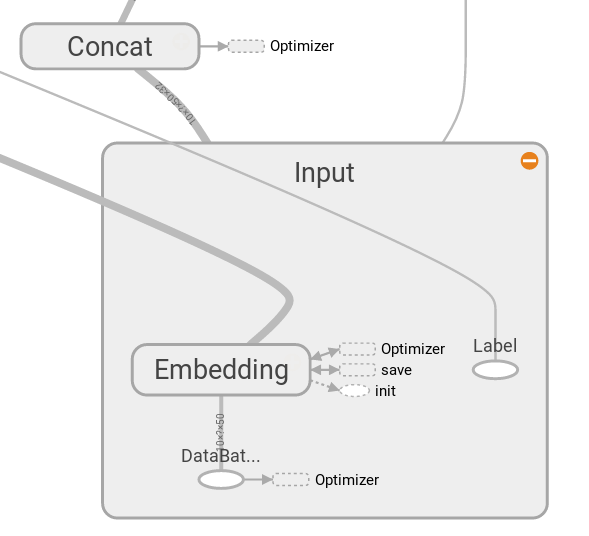
\includegraphics[width=0.8\textwidth]{graphic/nolstm2.png}
\caption{NOLSTM模型Input层 \label{nolstm2}}
\end{center}
\end{figure}
\begin{figure}[!hbp]
\begin{center}
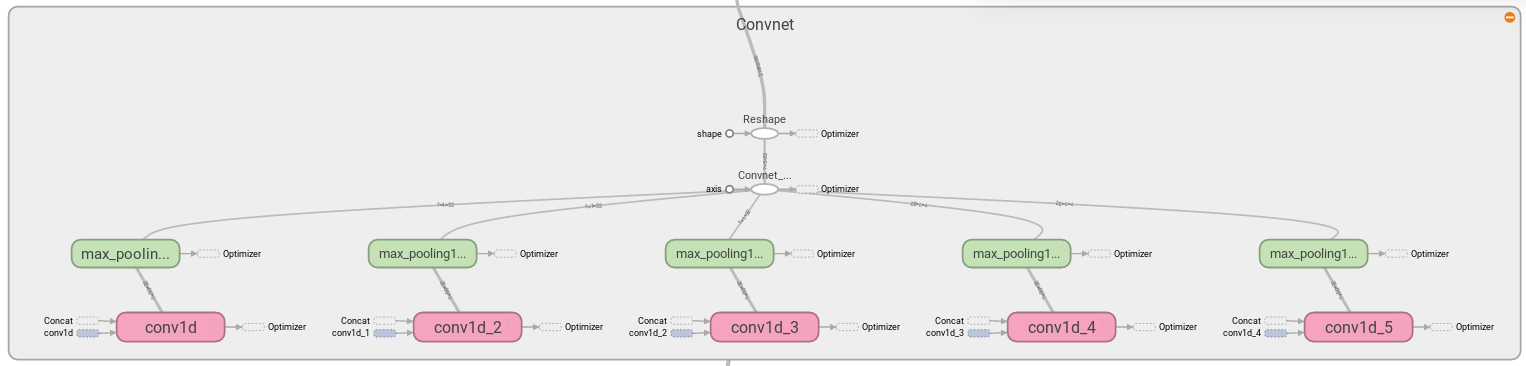
\includegraphics[width=0.8\textwidth]{graphic/nolstm3.png}
\caption{NOLSTM模型卷积层 \label{nolstm3}}
\end{center}
\end{figure}
\begin{figure}[!hbp]
\begin{center}
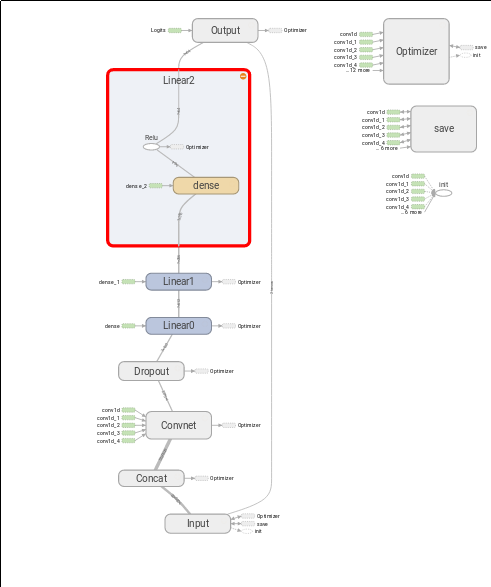
\includegraphics[width=0.8\textwidth]{graphic/nolstm4.png}
\caption{NOLSTM模型输出层 \label{nolstm3}}
\end{center}
\end{figure}
\subsection{模型主要流程}
模型分为训练模式与测试模式:\par
在训练模式下,基本步骤为:\par
\begin{enumerate}
\item 数据生成器按不同的语言要求生成输入特征,对超过限定长度的语句直接截断,以语句前半部分生成输入特征,实践证明往往前半部分已经拥有足够判断情感极性的信息。
\item 模型将这些特征通过输入层和连接层转化为统一的向量,计算误差。
\item 通过优化函数Optimizer,将误差反向传播以训练参数。
\item 每隔特定步数,对验证集进行测试,测试时不启动反向传播。
\item 若验证集精度大于已有最好精度,保存该模型,同时在测试集上进行测试,本文认为在测试集上的精度衡量了其泛化能力。
\end{enumerate}
在测试模式下,基本步骤为:\par
\begin{enumerate}
\item 载入模型。
\item 使用数据生成器将单一语句转化为输入特征。
\item 计算各标签的概率,即Output层中的Logits,输出概率最高的标签。
\end{enumerate}
\subsection{模型主要改进}
相对于C\& W模型,本文根据情感分析任务对模型进行了特化。
\begin{enumerate}
\item 待编码特征通过word2vec进行训练,以加快训练速度。
\item 选择全局池化,而不是C\& W模型中的时延模型,以舍弃语法特征。
\item 直接截断语句,取前半部分计算,以加快计算速度,减少空间损耗。
\end{enumerate}
\section{CLSTM模型}
由于文本是不定长的离散序列,故RNN适应于对文本建模和分析。本文使用卷积神经网络结合LSTM模型实现了基于循环神经网络的情感分类模型,简称为CLSTM模型,以与NOLSTM相区别。
\section{神经网络结构}
如图\ref{clstm1},CLSTM模型主要分为八层,输入层,连接层,卷积层,池化层,Dropout层,第一线性层,LSTM单元层(图\ref{clstm2}),第二线性层。其中输入层,连接层,卷积层,池化层与NOLSTM模型相同。采用与NOLSTM模型相同的卷积层可能违反直觉,因为RNN能够有效利用基于时序的局部特征,但实际上恰恰相反,不使用卷积神经网络或者使用局部池化及堆叠局部池化反而导致模型后期精度下降,这可能同样由语法结构可能反而会导致过拟合这一原因导致的。在实际测试中,该网络结构的性能较为出色。\par
在对输出特征进行dropout之后,特征首先进入第一线性层而不是LSTM层,以减少特征数量,抽取高级特征,便于LSTM层进行保存。最后,模型通过第二线性层以及输出层预测和计算输出结果。总而言之,LSTM层取代了NOLSTM模型中的第二线性层。
\subsection{模型主要流程}
模型分为训练模式与测试模式,设stepNum为LSTM单元迭代次数,在训练模式下,基本步骤为:\par
\begin{enumerate}
\item 数据生成器按不同的语言要求生成stepNum步输入特征。
\item 执行第3-4步直到该batch中的句子全部遍历完毕。
\item 模型将stepNum步特征全部通过输入层和连接层转化为统一的向量,计算误差。
\item 通过优化函数Optimizer,将误差反向传播以训练参数。
\item 每隔特定步数,对验证集进行测试,测试时不启动反向传播。
\item 若验证集精度大于已有最好精度,保存该模型,同时在测试集上进行测试,本文认为在测试集上的精度衡量了其泛化能力。
\end{enumerate}
在测试模式下,基本步骤为:\par
\begin{enumerate}
\item 载入模型。
\item 使用数据生成器将单一语句转化为stepNum步输入特征。
\item 重复执行第3-4步直到该句子被遍历完毕。
\item 计算各标签的概率,即Output层中的Logits,输出概率最高的标签。
\end{enumerate}
\begin{figure}[!hbp]
\begin{center}
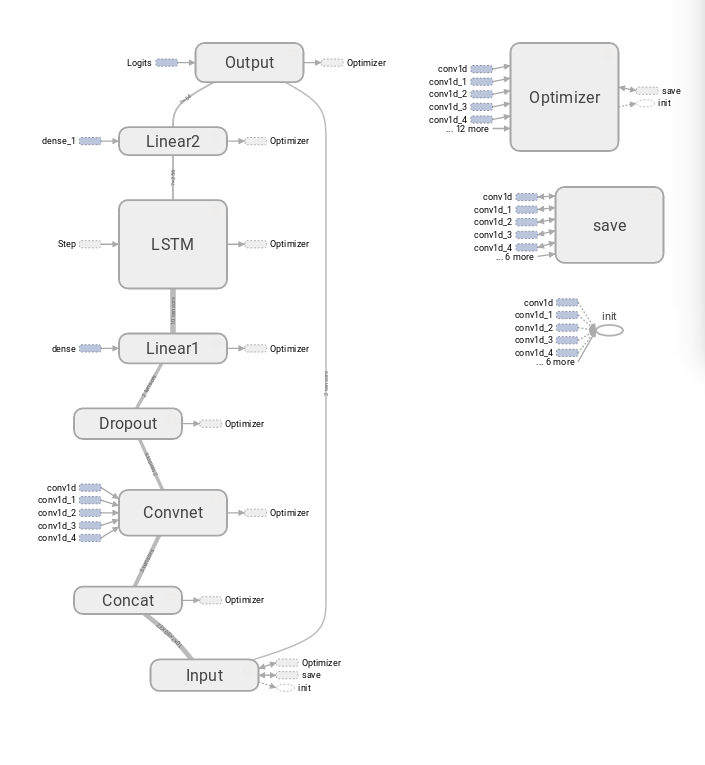
\includegraphics[width=0.8\textwidth]{graphic/clstm1.png}
\caption{CLSTM模型整体结构 \label{clstm1}}
\end{center}
\end{figure}
\begin{figure}[!hbp]
\begin{center}
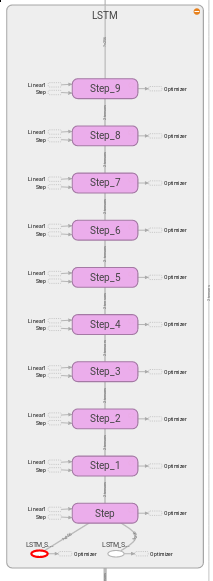
\includegraphics[width=0.4\textwidth]{graphic/clstm2.png}
\caption{CLSTM模型LSTM层 \label{clstm2}}
\end{center}
\end{figure}
\section{模型主要优化}
CLSTM模型结合了LSTM模型与卷积神经网络,能够在提取全局短语特征的同时处理不定长序列。相较于NOLSTM模型,它能更好地利用自然语言地序列属性,训练更少但更有效的参数。实践中,CLSTM模型往往比NOLSTM模型取得更好的成果。
%\chapter{结果分析}\thispagestyle{fancy}
本章主要对三个模型的准确率和时空复杂度进行测评,此外,本章对神经网络模型中的各项参数进行了分析。
\section{模型分析} \label{sec:modeleval}
\subsection{实验条件}
为了证实文本提出的知识模型,NOLSTM模型和CLSTM模型的有效性,本章使用NLPCC 2014的SCDL数据集和用于展示的携程数据集进行测评,实验条件如下:\par
运行参数:\par
\begin{itemize}
\item 操作系统: ubuntu16.10 64位
\item 运行平台: tensorflow v1.1
\item 磁盘空间: 1.9 TB
\item 内存空间: 32 GB
\item 处理器: Intel Core i7-6700 3.40 GHz x 8
\end{itemize}
\par 
神经网络参数:


\begin{center}
\begin{longtabu} to \textwidth{X|X|X|X}
\hline
参数名称 & 模型 & 数据集 & 参数值
\\\hline
离散特征编码长度 & - & CLSTM和NOLSTM & 32
\\\hline
稀有词限定最低频度 & NLPCC2014SCDL中文数据集 & CLSTM,NOLSTM & 'all': 7, 'nt': 12, 'ns': 12, 'nrf':12, 'nto': 12, 'null': 12, None: 12
\\\hline
稀有词限定最低频度 & NLPCC2014SCDL中文数据集 & CLSTM,NOLSTM & 'all': 7
\\\hline
稀有词限定最低频度 & 携程数据集 & CLSTM,NOLSTM & 'all': 7
\\\hline
batch大小 & - & CLSTM和NOLSTM & 200句
\\\hline
步数 & - & CLSTM & 10
\\\hline
每步包含词数 & NLPCC2014SCDL中文数据集 & CLSTM & 50
\\\hline
每步包含词数 & NLPCC2014SCDL英文数据集 & CLSTM & 250
\\\hline
每步包含词数 & 携程数据集 & CLSTM & 50
\\\hline
词数 & NLPCC2014SCDL中文数据集 & NOLSTM & 200
\\\hline
词数 & NLPCC2014SCDL英文数据集 & NOLSTM & 1000
\\\hline
词数 & 携程数据集 & NOLSTM & 250
\\\hline
LSTM单元维度 & - & CLSTM & 256
\\\hline
线性层0维度 & - & NOLSTM & 512
\\\hline
线性层1维度 & - & CLSTM,NOLSTM & 256
\\\hline
线性层2维度 & - & CLSTM,NOLSTM & 64
\\\hline
初始学习速率 & - & CLSTM & 1.0
\\\hline
初始学习速率 & - & NOLSTM & 0.1
\\\hline
Dropout Keep Rate & - & CLSTM,NOLSTM & 0.6
\\\hline
验证间隔 & NLPCC2014SCDL & CLSTM,NOLSTM & 40步 
\\\hline
验证间隔 & 携程数据集 & CLSTM,NOLSTM & 200步
\\\hline
\end{longtabu}
\end{center}

\subsection{精度分析}
本文中验证标准为准确率,即分类正确的语句占测试集的百分比。\par
神经网络模型的测试方法为:\par
\begin{itemize}
\item NLPCC 2014的SCDL数据集在官方训练集上进行封闭训练,使用官方测试集作为测试集。
\item 携程数据集使用5-fold进行测试,依次选取其中一个子集作为验证集,一个子集作为测试集,最终的测试准确率为五次平均。
\end{itemize}


准确度结果如下表:
\begin{center}
\begin{longtabu} to \textwidth{X|X|X|X|X}
\hline
数据集名称 & 知识模型 & CNNPL & CNNLSTMPL & NLPCC-best
\\\hline
携程数据集 & 69.9\% & 74.3\% & 76.7\% & -
\\\hline
NLPCC 2014 SCDL 中文 & 69.7\% & 76.3\% & 77.5\% & 76.9\%
\\\hline
NLPCC 2014 SCDL 英文 & 76.2\% & 85.2\% & 86.3\% & 86.0\%
\\\hline
\end{longtabu}
\end{center}


其中NLPCC-best为官方正式比赛中最高的准确率\cite{nlpccres},这里由于NLPCC测试集中正向:负向为1:1,所以该准确率为$\frac{NP + PP}{2}$。\par
从表中可以得出,CLSTM和NOLSTM在数据集上的表现都较好,接近或略高于第一名的准确度,知识模型的表现略差。由此可以证明CLSTM和NOLSTM模型是有效的,而知识模型还需要再加以改进。同时,CLSTM模型的精度往往高于NOLSTM模型,这可能是由于CLSTM模型一次处理的单词较少,从而需要训练的参数更少,而且CLSTM模型更能利用自然语言的序列信息。综合来看,基于深度学习的神经网络不需要大量语言学知识,也不依赖于情感词典和语法分析工具,却可以通过学习特征表达的方式达到超过传统的基于知识的模型的性能。\par

\subsection{时空复杂度分析}
时间消耗如下表(取到达最高精度的时间):\par
\begin{center}
\begin{longtabu} to \textwidth{X|X|X|X} 
\hline
数据集名称 & 知识模型 & NOLSTM & CLSTM
\\\hline
携程数据集 & 18770s & 1921s & 5350s % 
\\\hline
NLPCC2014SCDL中文 & 2768s & 564s & 1366s % 
\\\hline
NLPCC2014SCDL英文 & 3125s & 1389s & 3138s % 
\\\hline
\end{longtabu}
\end{center}
\par
由于CLSTM模型需要反复迭代,因此CLSTM模型速度较LSTM模型更差,由于训练策略的原因,CLSTM模型并不特意将长度相似的语句放在同一个batch中,这导致短句处理完毕后模型需要接受短句的补零,如果长句均匀分布在训练集内,就会导致训练速度下降。\par
知识模型速度较慢的原因可能有四点:1. 知识模型启动时需要同时启动ansj和stanfordParser的中英版本,耗时较多。2. 知识模型在实现中不直接使用分词后的词语,而是主动调用分词工具,因此导致时间较慢。 3. 知识模型需要对每条语句建立语法树,因此耗时较多。 4. 知识模型通过jpype调用java实现,中间操作较多,且jpype需要管理和启动java虚拟机。\par
\begin{center}
\begin{longtabu} to \textwidth{X|X|X|X}
\hline
数据集名称 & 知识模型 & NOLSTM & CLSTM \\
\hline
NLPCC2014SCDL中文 & 12276572K & 3733108K & 5905060K \\
\hline
NLPCC2014SCDL英文 & 12276572K & 3408696K & 5686756K
\\\hline
\end{longtabu}
\end{center}


从表中可以总结出在三种模型中NOLSTM的速度最快,空间消耗率是最低的,因此,可以得出结论,在文本较短情感较为强烈时,使用NOLSTM模型是节约时间和空间的做法,而如果需要处理不定长的文本,或者对精度要求较高,则应当使用CLSTM模型。\par
\section{参数分析}
本节分析对比神经网络模型的各种基本参数以及策略,由于神经网络训练较为费时,所以本节选取NOLSTM模型,使用NLPCC2014SCDL中文数据集进行训练,以对比不同参数或策略条件下的精度,得出最优参数或策略。
\subsection{初始编码策略}
在预处理过程中,本文使用word2vec训练待编码的离散特征向量。为了探究该步骤是否存在意义,本文使用NOLSTM模型,在参数相同的情况下分别运行了三次,第一次使用word2vec初始化编码,第二次使用零矩阵初始化编码,第三次则使用截断的正态分布随机初始化向量,取mean=0,stddev=0.1,准确率随训练过程的变化如图\ref{femb}:


通过观察该图内的三条曲线,可以发现word2vec的编码准确率较高,正态分布的编码准确率次之,但也呈现上升趋势,并且随时间逐渐接近word2vec编码的准确率,而零矩阵则无法训练,几乎保持为一条直线。综上所述,可以认为word2vec编码加快了训练速度,并且可能提高模型准确率。因此,使用word2vec初始化编码是有意义的。
\begin{center}
\begin{figure}[!hbp]
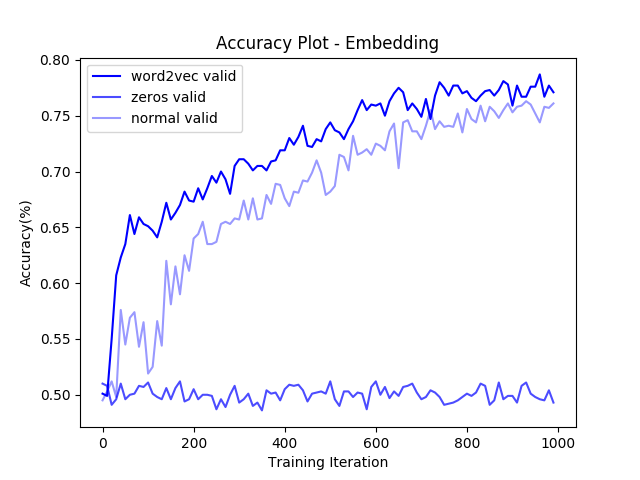
\includegraphics[width=0.8\textwidth]{graphic/emb.png}
\caption{编码-准确率变化图 \label{femb}}
\end{figure}
\end{center}
\subsection{优化函数选择}
本文中NOLSTM模型和CLSTM模型都使用ADAM算法作为优化函数。本小节中对本文中使用的优化函数做出评估,分别使用SGD算法,ADADELTA算法和ADAM算法在同样的参数下各自训练NOLSTM模型,得到准确率随时间的变化曲线如图\ref{fopt}:


通过观察图中的三条曲线,可以发现ADAM的训练速度和准确率都最高,SGD次之,而ADADELTA最慢。实际上,这是因为ADADELTA算法陷入了局部最小值点。综上所述,可以认为选择ADAM作为优化函数是正确的。实际上,SGD算法也是学术研究中较为常用的算法,如果人工配置的学习率足够强大,往往能够得到自适应梯度的优化函数所不能得到的效果。
\begin{center}
\begin{figure}[!hbp]
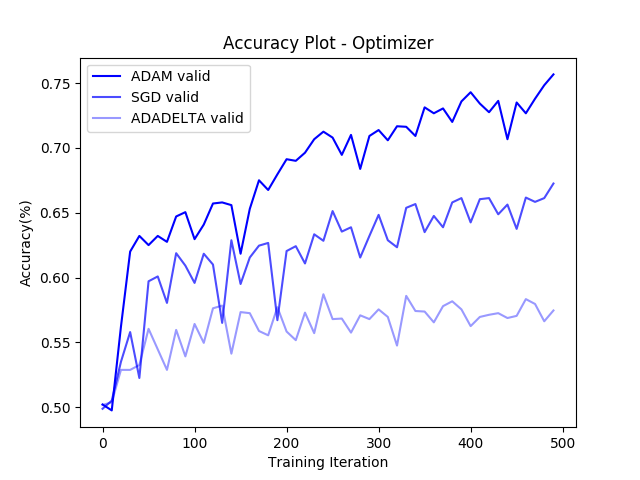
\includegraphics[width=0.8\textwidth]{graphic/opt.png}
\caption{优化函数-准确率变化图 \label{fopt}}
\end{figure}
\end{center}
\subsection{激活函数选择}
本文中模型都使用ReLU算法作为线性层之间的激活函数。本小节中对本文中使用的激活函数做出评估,分别使用ReLU算法,tanh算法和sigmoid算法在同样的参数下各自作为线性层之间的激活函数训练NOLSTM模型,得到准确率随时间的变化曲线如图\ref{fnonlinear}:


在训练过程中,三种函数所对应的模型都保持近似于一致的上升趋势,但当训练进入后期,接近最高准确率时,ReLU也即颜色最深的曲线的准确率保持最高,因此,可以认为ReLU相较于sigmoid函数和tanh函数来说更适宜作为线性层之间的激活函数。这可能与ReLU具有单侧抑制和稀疏激活性有关。
\begin{center}
\begin{figure}[!hbp]
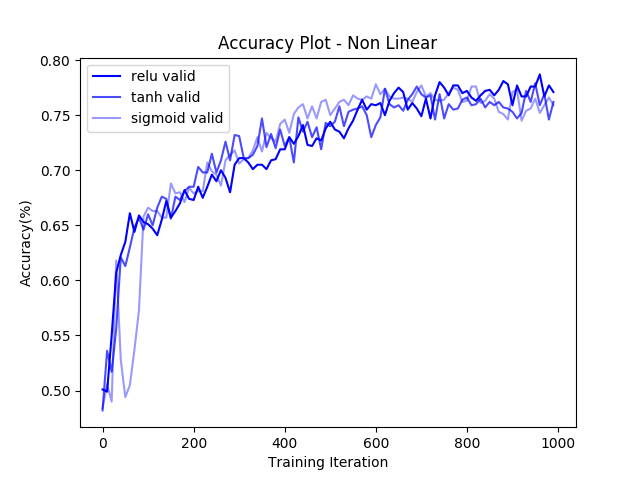
\includegraphics[width=0.8\textwidth]{graphic/nonlinear.png}
\caption{激活函数-准确率变化图 \label{fnonlinear}}
\end{figure}
\end{center}
\subsection{是否过滤稀有词} \label{sec:rareword}
本文在预处理过程中会对离散特征做过滤稀有词操作,即按照词性和最低频度将频度小于此词性的最低频度的离散特征转化为一个特殊的词,"RAREWORD"。本小节探讨该操作的必要性。


如图\ref{frareword},明显,使用全部单词,不进行稀有词过滤的模型准确率较低,泛化性能较差。从另一方面来说,例如数据集中只有一条负向文本中出现了"北京饭店"这个稀有词汇,则神经网络极有可能将"北京饭店"学习为负向情感词汇,但实际上该词汇是中性的实体词汇。通过过滤稀有词,模型能够尽力保证词汇在多种句式中出现,从而能够学习到词汇的真正含义,避免被标注影响,也能帮助抽取高级特征。
\begin{center}
\begin{figure}[!hbp]
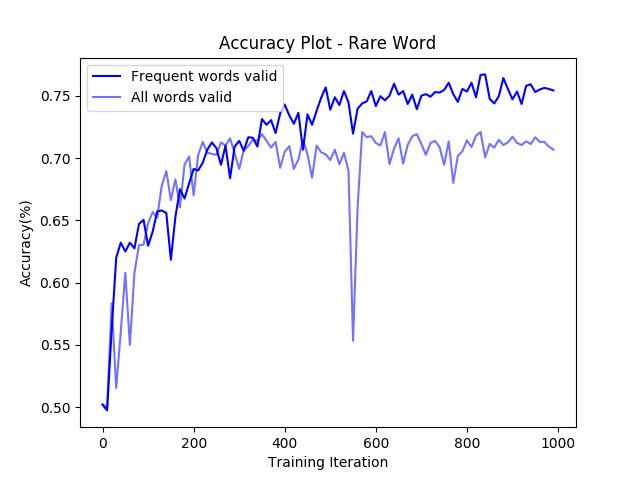
\includegraphics[width=0.8\textwidth]{graphic/rareword.png}
\caption{是否过滤稀有词-准确率变化图 \label{frareword}}
\end{figure}
\end{center}
\subsection{是否使用dropout}
dropout函数随机使输出单元的一部分为0,即使其输出无效。使用dropout函数往往能够迫使模型学习更加健壮的特征,避免被局部特征所误导,可以减轻局部最小值的问题。但dropout本身可能导致模型精度无法提升等问题。本小节讨论神经网络模型在处理情感分类任务中dropout是否必要。如图\ref{fdropout},分别进行了两次训练,一次dropout 保持不变的可能性设置为0.6,另一次不设置dropout。


从图中可以看出,尽管在训练的早期阶段无dropout的模型准确率上升速度更加快,但在后期使用dropout的算法能明显增加准确度。因此,可以认为使用dropout不仅能影响到准确率,而且还是必要的,能够帮助泛化。在实践中,为了体现dropout的效果,本文将之设为0.6。
\begin{center}
\begin{figure}[!hdp]
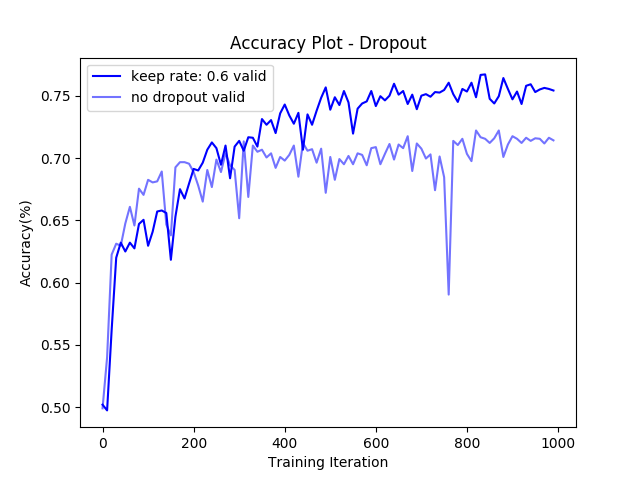
\includegraphics[width=0.8\textwidth]{graphic/dropout.png}
\caption{有无Dropout-准确率变化图 \label{fdropout}}
\end{figure}
\end{center}
\subsection{卷积核研究}
实际上,在没有接触到NLPCC2014的任务集之前,笔者认为局部池化,尤其是堆叠卷积网络加池化的能够抽取出高级的语法特征,更适应于情感分类任务,但实际上,在本文所做过的测试中,核较小的卷积加全局池化的性能往往优于堆叠卷积网络加池化。


本小节使用一种特殊的方法表示卷积核,【3,4,5,6,7】(【-1,-1,-1,-1,-1】)代表只有一维卷积,分别是核大小为3,4,5,6,7的的卷积,每个卷积输出使用全局池化处理,【2,3,5】(【2,3,5】)代表只有一维卷积,分别是核为2,步长为1的,由大小为2,步长为2的最大池化层处理的卷积输出,核为3,步长为1的,使用大小为3,步长为3的最大池化进行处理的卷积输出和核与池化层,步长都为5的卷积输出。【2,3,5】(【2,3,5】),【1,2,3】(【1,2,3】)则代表在【2,3,5】(【2,3,5】)输出的特征上,分别做卷积核大小为1,2,3,池化层大小和步长对应为1,2,3的卷积->池化操作。


本文进行了一系列实验,相关准确度如下:


\begin{itemize}
\item 【3,5,6,7,9】 (【-1,-1,-1,-1,-1】): 0.75
\item 【3,5,7,9】(【-1,-1,-1,-1】):0.73
\item 【1】(【1】): 0.66
\item 【2,3】(【2,3】),【3,5,6,7,9】 (【-1,-1,-1,-1,-1】):0.71
\item 【2,3,5】(【2,3,5】),【1,2,3】(【2,3,5】),【1,2,3】(【2,3,5】):0.75
\item 【3,5,7】(【3,5,7】),【1,2,3】(【2,3,5】),【1,2,3】(【2,3,5】):0.73
\item 【2,3,5】(【2,3,5】),【1,2,3】(【1,2,3】): 0.68
\item 【2,2,2,2】(【2,2,2,2】): 0.56
\item 【2,2,2,2】(【2,2,2,-1】): 0.55
\item 【2,3,4】: 0.63
\item 【3,4,5】: 0.64
\item 【4,5,6】: 0.54
\item 【2,3,4】(【2,3,4】): 0.62
\item 【3,4,5】(【3,4,5】)
\item 【9,11,13】(【-1,-1,-1】): 0.68
\item 【2,3,5】(【-1,-1,-1】): 0.65
\item ...
\end{itemize}

在实验中,可以发现堆叠卷积神经网络并不能改进模型性能。综合考虑后,模型决定采用【3,5,6,7,8】(【-1,-1,-1,-1,-1】),因为它不仅精度最高,而且表现更为稳定,训练速度也较快。当卷积核为1,池化层也为1时,模型相当于LSTM模型,在实践中,该模型效果不佳,不能泛化出应有结果。



%%参考文献
\clearpage
\phantomsection

\addcontentsline{toc}{chapter}{参考文献}
{\songti\zihao{5}
\bibliographystyle{IEEEtran}
\bibliography{IEEEabrv,ref/referenceUndergraduate}
}
%致谢
\clearpage
\phantomsection
\addcontentsline{toc}{chapter}{致\quad{}\quad{}谢}
\chapter*{致\qquad 谢}\thispagestyle{fancy}
\songti\zihao{-4} 

	本毕设的完成得到了很多人的帮助。首先要感谢吴国仕老师的指导与帮助,老师的认真与负责使我受益良多,毕设后期没有听从您不要涉足实体领域的劝告,结果果然惨淡首尾。同时也要感谢李晶老师,在跟随李晶老师和吴国仕老师做大学生创新竞赛时,我对这一领域有了基本的了解。同样也感谢大创中一起努力过的小伙伴,是大家的辛苦付出,使我们最终完成了整个项目。接着需要感谢我的各位室友,感谢她们在四年来的支持与鼓励,拥有这样的室友是我的荣幸,希望之后还能一直是朋友。同时,也要感谢默默支持我的两位好友,马和翟。最后,感谢父母家人的宽容与耐心,谢谢你们的鼓励与支持。


%
%%附录
\clearpage
\phantomsection
\addcontentsline{toc}{chapter}{附\quad{}\quad{}录}
\chapter*{附\qquad 录}
\section*{附录~1\quad	分词工具准确率测试} \label{appendix:parsercompare}
\begin{center}  
\begin{longtabu} to \textwidth{X|X[6]} 
\hline
工具 & 结果 \\
\hline
语句 & 很好,曲屏太带感了,流畅度可以\\
ansj\newline (Nlp模式) & 很,d,好,a,,,w,曲屏太带感,nw,了,ul,,,w,流畅,a,度,q,可以,v\\
thulac\newline (精准模式) & 很,d,好,a,,,w,曲屏,n,太带感,n,了,u,,,w,流畅度,id,可以,v\\
jieba\newline (精准模式) & 很,d,好,a,,,x,曲屏,nr,太,d,带感,v,了,ul,,,x,流畅,a,度,zg,可以,v\\
\hline
语句 & 很好啊,京东牛逼。物流也快,东西也好。\\
ansj\newline (Nlp模式) & 很,d,好,a,啊,y,,,w,京东,ns,牛逼,nw,。,w,物流,n,也,d,快,a,,,w,东西,n,也好,y,。,w\\
thulac\newline (精准模式) & 很,d,好,a,啊,u,,,w,京,j,东,f,牛,n,逼,v,。,w,物流,n,也,d,快,a,,,w,东西,n,也好,u,。,w\\
jieba\newline (精准模式) & 很,d,好,a,啊,y,,,x,京东,ns,牛,n,逼,v,。,x,物流,n,也,d,快,a,,,x,东西,n,也好,y,。,x\\
\hline
语句 & 包装挺好。看上去也不错\\
ansj\newline (Nlp模式) & 包装,vn,挺,d,好,a,。,w,看上去,v,也,d,不错,a\\
thulac\newline (精准模式) & 包装,v,挺,d,好,a,。,w,看上去,v,也,d,不错,a\\
jieba\newline (精准模式) & 包装,n,挺,d,好,a,。,x,看上去,v,也,d,不错,a\\
\hline
语句 & 手机反应挺快,用了十天左右,屏幕出现彩条,把膜撕掉以后,发现手机坏了,退货,损失了一个手机膜!\\
ansj\newline (Nlp模式) & 手机,n,反应,vn,挺快,v,,,w,用,p,了,ul,十天,m,左右,m,,,w,屏幕,n,出现,v,彩条,nz,,,w,把,p,膜,n,撕掉,nz,以后,f,,,w,发现,v,手机,n,坏,a,了,ul,,,w,退货,v,,,w,损失,n,了,ul,一个,m,手机,n,膜,n,!,w\\
thulac\newline (精准模式) & 手机,n,反应,v,挺,d,快,a,,,w,用,p,了,u,十,m,天,q,左右,m,,,w,屏幕,n,出现,v,彩条,n,,,w,把,p,膜,n,撕掉,v,以后,f,,,w,发现,v,手机,n,坏,a,了,u,,,w,退货,v,,,w,损失,v,了,u,一个,m,手机,n,膜,n,!,w\\
jieba\newline (精准模式) & 手机,n,反应,vn,挺快,v,,,x,用,p,了,ul,十天,m,左右,f,,,x,屏幕,n,出现,v,彩条,nz,,,x,把,p,膜,n,撕掉,nz,以后,f,,,x,发现,v,手机,n,坏,a,了,ul,,,x,退货,v,,,x,损失,n,了,ul,一个,m,手机,n,膜,n,!,x\\
\hline
语句 & 买了之后打不开卡槽\\
ansj\newline (Nlp模式) & 买,v,了,ul,之后,f,打不开,v,卡槽,nw\\
thulac\newline (精准模式) & 买,v,了,u,之后,f,打,v,不,d,开,v,卡槽,n\\
jieba\newline (精准模式) & 买,v,了,ul,之后,f,打不开,v,卡槽,nw\\
\hline
语句 & 还算性价比较高的,可以推荐\\
ansj\newline (Nlp模式) & 还算,v,性价,nw,比较,d,高,a,的,uj,,,w,可以,v,推荐,v\\
thulac\newline (精准模式) & 还,d,算,v,性价,n,比较,d,高,a,的,u,,,w,可以,v,推荐,v\\
jieba\newline (精准模式) & 还算,v,性价,nw,比较,d,高,a,的,uj,,,x,可以,v,推荐,v\\
\hline
语句 & 入住北京天坛全季酒店非常满意,很温馨,来北京首选的酒店,房间很温暖很干净,酒店服务很好,非常干净,临近小区安静,睡的很舒服\\
ansj\newline (Nlp模式) & 入住,v,北京天坛全季酒店,nt,非常,d,满意,v,,,w,很,d,温馨,a,,,w,来,v,北京,ns,首选,v,的,uj,酒店,n,,,w,房间,n,很,d,温暖,an,很,d,干净,a,,,w,酒店,n,服务,vn,很,d,好,a,,,w,非常,d,干净,a,,,w,临近,v,小区,n,安静,a,,,w,睡,v,的,uj,很,d,舒服,a\\
thulac\newline (精准模式) & 入住,v,北京,ns,天坛,ns,全季,n,酒店,n,非常,d,满意,v,,,w,很,d,温馨,a,,,w,来,v,北京,ns,首选,v,的,u,酒店,n,,,w,房间,n,很,d,温暖,a,很,d,干净,a,,,w,酒店,n,服务,v,很,d,好,a,,,w,非常,d,干净,a,,,w,临近,v,小区,n,安静,a,,,w,睡,v,的,u,很,d,舒服,a\\
jieba\newline (精准模式) & 入住,v,北京,ns,天坛,ns,全季,nw,酒店,n,非常,d,满意,v,,,x,很,zg,温馨,a,,,x,来,v,北京,ns,首选,v,的,uj,酒店,n,,,x,房间,n,很,zg,温暖,an,很,zg,干净,a,,,x,酒店,n,服务,vn,很,d,好,a,,,x,非常,d,干净,a,,,x,临近,v,小区,n,安静,a,,,x,睡,v,的,uj,很,a,舒服,a\\
\hline
语句 & 这次的入住,让我印象颇好。深冬寒冷的北京,王府细致温暖的服务让我暖心。虽然设施略显陈旧了,但是卫生情况良好,早餐厅、健身房、前台是这几天接触最多的部门,都彬彬有\\
ansj\newline (Nlp模式) & 这次,r,的,uj,入住,v,,,w,让,v,我,r,印象,n,颇,d,好,a,。,w,深冬,t,寒冷,a,的,uj,北京,ns,,,w,王府,n,细致,a,温暖,an,的,uj,服务,vn,让,v,我,r,暖心,nw,。,w,虽然,c,设施,n,略显,d,陈旧,a,了,ul,,,w,但是,c,卫生,an,情况,n,良好,a,,,w,早餐厅,n,、,w,健身房,n,、,w,前台,n,是,v,这,r,几天,m,接触,v,最多,ad,的,uj,部门,n,,,w,都,d,彬彬有,nw\\
thulac\newline (精准模式) & 这次,r,的,u,入住,v,,,w,让,v,我,r,印象,n,颇,d,好,a,。,w,深冬,t,寒冷,a,的,u,北京,ns,,,w,王府,n,细致,a,温暖,a,的,u,服务,v,让,v,我,r,暖,v,心,n,。,w,虽然,c,设施,n,略,d,显,v,陈旧,a,了,u,,,w,但是,c,卫生,a,情况,n,良好,a,,,w,早餐厅,n,、,w,健身房,n,、,w,前台,n,是,v,这,r,几,m,天,q,接触,v,最,d,多,a,的,u,部门,n,,,w,都,d,彬彬有,id\\
jieba\newline (精准模式) & 这次,r,的,uj,入住,v,,,x,让,v,我,r,印象,n,颇,d,好,a,。,x,深冬,t,寒冷,a,的,uj,北京,ns,,,x,王府,n,细致,a,温暖,an,的,uj,服务,vn,让,v,我,r,暖,a,心,n,。,x,虽然,c,设施,n,略显,d,陈旧,a,了,ul,,,x,但是,c,卫生,an,情况,n,良好,a,,,x,早餐厅,n,、,x,健身房,n,、,x,前台,n,是,v,这,r,几天,m,接触,v,最多,ad,的,uj,部门,n,,,x,都,d,彬彬,nz,有,v\\
\hline
语句 & 房间太脏,灰尘很大。\\
ansj\newline (Nlp模式) & 房间,n,太,d,脏,a,,,w,灰尘,n,很大,d,。,w\\
thulac\newline (精准模式) & 房间,n,太,d,脏,a,,,w,灰尘,n,很,d,大,a,。,w\\
jieba\newline (精准模式) & 房间,n,太脏,n,,,x,灰尘,n,很大,d,。,x\\
\hline
语句 & 环境好交通方便\\
ansj\newline (Nlp模式) & 环境,n,好,a,交通,n,方便,a\\
thulac\newline (精准模式) & 环境,n,好,a,交通,n,方便,a\\
jieba\newline (精准模式) & 环境,n,好,a,交通,n,方便,a\\
\hline
语句 & 看了一遍又一遍,还是挺喜欢的\\
ansj\newline (Nlp模式) & 看,v,了,ul,一遍,m,又,d,一遍,m,,,null,还是,c,挺,d,喜欢,v,的,uj\\
thulac\newline (精准模式) & 看,v,了,u,一,m,遍,q,又,d,一,m,遍,q,,,w,还是,c,挺,d,喜欢,v,的,u\\
jieba\newline (精准模式) & 看,v,了,ul,一遍,m,又,d,一遍,m,,,x,还是,c,挺,d,喜欢,v,的,uj\\
\hline
语句 & 快快快!盼望《大明英烈》,《白眉大侠》,《三侠剑》,《封神演义》等等\\
ansj\newline (Nlp模式) & 快快快,nw,!,w,盼望,v,《,w,大明,nz,英烈,n,》,w,,,w,《,w,白眉,nz,大侠,n,》,w,,,w,《,w,三侠,nr,剑,n,》,w,,,w,《,w,封神演义,nz,》,w,等等,u\\
thulac\newline (精准模式) & 快,d,快,d,快,a,!,w,盼望,v,《,w,大明英烈,n,》,w,,,w,《,w,白眉大侠,id,》,w,,,w,《,w,三侠剑,nz,》,w,,,w,《,w,封神演义,nz,》,w,等等,u\\
jieba\newline (精准模式) & 快快快,nw,!,x,盼望,v,《,x,大明,nz,英烈,n,》,x,,,x,《,x,白眉,nz,大侠,n,》,x,,,x,《,x,三侠,nr,剑,n,》,x,,,x,《,x,封神演义,nz,》,x,等等,u\\
\hline
语句 & 你无权强加民意,应该叫《你不高兴!》
哗众取宠,为了你的经济利益吧?
赚钱要正当,不是叫嚣几句不高兴就行的,何况,你无权叫“中国”不高兴!
鄙视你,无知且无畏、胆大妄为的作者!
赚这种钱,有意思吗?\\
ansj\newline (Nlp模式) & 你,r,无权,v,强加,v,民意,n,,,w,应该,v,叫,v,《,w,你,r,不,d,高兴,a,!,w,》,w,哗众取宠,i,,,w,为了,p,你的,nt,经济,n,利益,n,吧,y,?,w,赚钱,v,要,v,正当,a,,,w,不是,c,叫嚣,v,几句,m,不,d,高兴,a,就,d,行,v,的,uj,,,w,何况,c,,,w,你,r,无权,v,叫,v,“,w,中国,ns,”,w,不,d,高兴,a,!,w,鄙视,v,你,r,,,w,无知,a,且,c,无畏,v,、,w,胆大妄为,i,的,uj,作者,n,!,w,赚,v,这种,r,钱,n,,,w,有意思,l,吗,y,?,w\\
thulac\newline (精准模式) & 你,r,无权,v,强加,v,民意,n,,,w,应该,v,叫,v,《,w,你,r,不,d,高兴,a,!,w,》,w,换行符,,哗众取宠,id,,,w,为了,p,你,r,的,u,经济,n,利益,n,吧,u,?,w,换行符,,赚钱,v,要,v,正当,v,,,w,不,d,是,v,叫嚣,v,几,m,句,q,不,d,高兴,a,就,d,行,a,的,u,,,w,何况,c,,,w,你,r,无权,v,叫,v,“,w,中国,ns,”,w,不,d,高兴,a,!,w,换行符,,鄙视,v,你,r,,,w,无知,a,且,c,无畏,v,、,w,胆大妄为,id,的,u,作者,n,!,w,换行符,,赚,v,这种,r,钱,n,,,w,有意思,id,吗,u,?,w\\
jieba\newline (精准模式) & 你,r,无权,v,强加,v,民意,n,,,x,应该,v,叫,v,《,x,你,r,不,d,高兴,a,!,x,》,x,换行符,x,哗众取宠,i,,,x,为了,p,你的,nt,经济,n,利益,n,吧,y,?,x,换行符,x,赚钱,v,要,v,正当,a,,,x,不是,c,叫嚣,v,几句,m,不,d,高兴,a,就行,v,的,uj,,,x,何况,c,,,x,你,r,无权,v,叫,v,“,x,中国,ns,”,x,不,d,高兴,a,!,x,换行符,x,鄙视,v,你,r,,,x,无知,a,且,zg,无畏,v,、,x,胆大妄为,i,的,uj,作者,n,!,x,换行符,x,赚,v,这种,r,钱,n,,,x,有意思,l,吗,y,?,x\\
\hline
语句 & 买了金属盒装的,里面有张抽奖券,按提示的网站登陆后查询号码,一直显示乱码,根本就无法得知你是否中奖!全是骗人的局!\\
ansj\newline (Nlp模式) & 买,v,了,ul,金属,n,盒装,vi,的,uj,,,null,里面,f,有,v,张抽奖,nw,券,ng,,,null,按,p,提示,v,的,uj,网站,n,登陆,v,后,f,查询,v,号码,n,,,null,一直,d,显示,v,乱码,nz,,,null,根本,a,就,d,无法,v,得知,v,你,r,是否,v,中奖,v,!,null,全,a,是,v,骗人,v,的,uj,局,n,!,null\\
thulac\newline (精准模式) & 买,v,了,u,金属,n,盒,g,装,v,的,u,,,w,里面,f,有,v,张,q,抽奖券,n,,,w,按,p,提示,v,的,u,网站,n,登陆,v,后,f,查询,v,号码,n,,,w,一直,d,显示,v,乱码,n,,,w,根本,d,就,d,无法,v,得知,v,你,r,是否,v,中奖,v,!,w,全,d,是,v,骗人,v,的,u,局,n,!,w\\
jieba\newline (精准模式) & 买,v,了,ul,金属,n,盒装,vi,的,uj,,,x,里面,f,有,v,张,nr,抽奖券,nz,,,x,按,p,提示,v,的,uj,网站,n,登陆,v,后,f,查询,v,号码,n,,,x,一直,d,显示,v,乱码,nz,,,x,根本,a,就,d,无法,v,得知,v,你,r,是否,v,中奖,vi,!,x,全,a,是,v,骗人,v,的,uj,局,n,!,x\\
\hline
语句 & 为什么不去进步步的MY STORY(私物语)呢????都等了很久了!!!!!希望卓越赶快去进货!!CD和CD+DVD的都进上!!!!地球人都知道步步的碟是中唱发行的!!!!卓越打造中国第一电子购物网不是靠吹的~!!快点进货吧!!!
日本流行乐坛第一而且唯一的女王滨崎步睽违2年的全新完整专辑“MY STORY 私物语”。收录“Moments 刹那”、“CAROLS 颂歌”、“INSPIRE 刺激”、“GAME 游戏”等四首日本公信榜冠军单曲,以及多首在日本搭配广告播出,引起热烈回响的的新曲“About You”、“walking proud”“my name\\
ansj\newline (Nlp模式) & 为什么,r,不,d,去,v,进步步,nw,的,uj,my,en,story,en,(,null,私,ag,物语,nz,),null,呢,y,?,null,?,null,?,null,?,null,都,d,等,u,了,ul,很久,d,了,ul,!,null,!,null,!,null,!,null,!,null,希望,v,卓越,a,赶快,d,去,v,进货,v,!,null,!,null,cd,en,和,c,cd,en,+,null,dvd,en,的,uj,都,d,进,v,上,f,!,null,!,null,!,null,!,null,地球,n,人,n,都,d,知道,v,步步,q,的,uj,碟是,nw,中,f,唱,v,发行,v,的,uj,!,null,!,null,!,null,!,null,卓越,a,打造,v,中国,ns,第一,m,电子,n,购物网,nz,不是,c,靠,v,吹,v,的,uj,~,null,!,null,!,null,快点,d,进货,v,吧,y,!,null,!,null,!,null,日本,ns,流行,v,乐坛,n,第一,m,而且,c,唯一,b,的,uj,女王,n,滨崎步睽违,nw,2年,m,的,uj,全新,b,完整,a,专辑,n,“,w,my,en,story,en,私,ag,物语,nz,”,w,。,w,收录,v,“,w,moments,en,刹那,t,”,w,、,w,“,w,carols,en,颂歌,n,”,w,、,w,“,w,inspire,en,刺激,v,”,w,、,w,“,w,game,en,游戏,n,”,w,等,u,四首,m,日本公信榜,nw,冠军,n,单曲,n,,,w,以及,c,多首,m,在,p,日本,ns,搭配,v,广告,n,播出,v,,,w,引起,v,热烈,a,回响,n,的的,nw,新曲,nz,“,w,about,en,you,en,”,w,、,w,“,w,walking,en,proud,en,”,w,“,w,my,en,name,en\\
thulac\newline (精准模式) & 为什么,r,不,d,去,v,进步,v,步,v,的,u,MY,x,STORY,x,(,w,私物,n,语,g,),w,呢,u,?,w,?,w,?,w,?,w,都,d,等,v,了,u,很,d,久,a,了,u,!,w,!,w,!,w,!,w,!,w,希望,v,卓越,a,赶快,d,去,v,进货,v,!,w,!,w,CD,x,和,c,CD,x,+,w,DVD,x,的,u,都,d,进,v,上,f,!,w,!,w,!,w,!,w,地球人,n,都,d,知道,v,步步,v,的,u,碟,g,是,v,中唱,j,发行,v,的,u,!,w,!,w,!,w,!,w,卓越,a,打造,v,中国,ns,第一,m,电子,n,购物网,n,不,d,是,v,靠,v,吹,v,的,u,~,w,!,w,!,w,快,a,点,q,进货,v,吧,u,!,w,!,w,!,w,换行符,,日本,ns,流行,v,乐坛,n,第一,m,而且,c,唯一,a,的,u,女王,n,滨崎步,np,睽违,v,2,m,年,q,的,u,全新,a,完整,a,专辑,n,“,w,MY,x,STORY,x,私物语,n,”,w,。,w,收录,v,“,w,Moments,x,刹那,t,”,w,、,w,“,w,CAROLS,x,颂歌,n,”,w,、,w,“,w,INSPIRE,x,刺激,v,”,w,、,w,“,w,GAME,x,游戏,n,”,w,等,u,四,m,首,q,日本,ns,公信榜,n,冠军,n,单曲,n,,,w,以及,c,多,a,首,q,在,p,日本,ns,搭配,v,广告,n,播出,v,,,w,引起,v,热烈,a,回响,v,的,u,的,u,新,a,曲,g,“,w,About,x,You,n,”,w,、,w,“,w,walking,x,proud,x,”,w,“,w,my,n,name,x\\
jieba\newline (精准模式) & 为什么,r,不,d,去,v,进步,vn,步,q,的,uj,MY,eng, ,x,STORY,eng,(,x,私,ag,物语,nz,),x,呢,y,?,x,?,x,?,x,?,x,都,d,等,u,了,ul,很久,d,了,ul,!,x,!,x,!,x,!,x,!,x,希望,v,卓越,a,赶快,d,去,v,进货,v,!,x,!,x,CD,eng,和,c,CD,eng,+,x,DVD,eng,的,uj,都,d,进上,v,!,x,!,x,!,x,!,x,地球,n,人,n,都,d,知道,v,步步,q,的,uj,碟是,nw,中,f,唱,v,发行,v,的,uj,!,x,!,x,!,x,!,x,卓越,a,打造,v,中国,ns,第一,m,电子,n,购物网,nz,不是,c,靠,v,吹,v,的,uj,~,x,!,x,!,x,快点,d,进货,v,吧,y,!,x,!,x,!,x,换行符,x,日本,ns,流行,v,乐坛,n,第一,m,而且,c,唯一,b,的,uj,女王,nnt,滨崎步,nz,睽违,nz,2,m,年,m,的,uj,全新,b,完整,a,专辑,n,“,x,MY,eng, ,x,STORY,eng, ,x,私,ag,物语,nz,”,x,。,x,收录,v,“,x,Moments,eng, ,x,刹那,t,”,x,、,x,“,x,CAROLS,eng, ,x,颂歌,n,”,x,、,x,“,x,INSPIRE,eng, ,x,刺激,v,”,x,、,x,“,x,GAME,eng, ,x,游戏,n,”,x,等,u,四首,m,日本公信榜,nw,冠军,n,单曲,n,,,x,以及,c,多首,m,在,p,日本,ns,搭配,v,广告,n,播出,v,,,x,引起,v,热烈,a,回响,n,的的,nw,新曲,nz,“,x,About,eng, ,x,You,eng,”,x,、,x,“,x,walking,eng, ,x,proud,eng,”,x,“,x,my,eng, ,x,name,eng\\
\hline
\end{longtabu}
\end{center}
\section*{附录~2\quad	词性还原和词根化工具准确率测试} \label{appendix:lemmacompare}

\begin{center}  
\begin{longtabu} to \textwidth{X|X|X|X|X}
\hline
单词 & Snowball & Lancaster & Porter & Stanford CoreNLP\\
\hline
get & get & get & get & get\\
\hline
got & got & got & got & get\\
\hline
gotten & gotten & got & gotten & get\\
\hline
gets & get & get & get & get\\
\hline
name & name & nam & name & name\\
\hline
named & name & nam & name & name\\
\hline
names & name & nam & name & name\\
\hline
nice & nice & nic & nice & nice\\
\hline
nicely & nice & nic & nice & nicely\\
\hline
\end{longtabu}
\end{center} 




\pagestyle{empty}
%外文译文
\chapter*{外\quad 文\quad 译\quad 文}
\pagestyle{empty}

\begin{center}
{\heiti\zihao{3}Natural Language Processing (almost) from Scratc

\textsl{By Ronan Collobert, Jason Weston, Leon Bottou, Michael Karlen, Koray Kavukcuoglu, Pavel Kuksa}

\heiti (几乎)从头开始自然语言处理
}
\end{center}

\zihao{-4}

\section*{摘要}
我们提出了一个统一通用的神经网络学习算法及框架,该框架可以被用于多种不同的自然语言处理任务,这些任务包括: 词性标注,词语分块,命名实体识别和语义角色标注。框架的这种通用性是通过避免以任务本身为中心的工作模式而取得的,也因此框架忽略了很多先验知识。与在任务特定的模式中让学者们小心翼翼地为人工挑选并生成输入特征不同,我们的系统只需要输入大量几乎未标注的训练语料,系统就能自动训练出内部表达方式,从而获取训练语料特征。以上工作也是之后我们建立的高性能计算要求低而且免费开源的标注系统的理论基础。
\section*{1. 简介}
是否存在一种数据结构,能够在一串英文文本通过电脑程序转化为该结构后完备且无歧义地描述该文本?在自然语言处理的大量问题中,学者们还没有对这种数据结构的形式达成共识。而在用人工智能解决这个基础问题之前,计算机科学家们必须解决该问题的简易版本,也就是从文本中抽取简单的描述文本信息的特定方面的特征表达方式。
这些简单的特征表达通常受到具体应用方式的启发,例如信息检索中使用的词袋变量。这些特征表达也可能是因为我们觉得它们能够捕获自然语言的某些通用普遍的信息所以被应用。它们可能描述句法信息(比如词性标注,词语分块和句法分析),也可能描述语法信息(比如词义消歧,语义角色标注,命名实体抽取和回指解析)。相关文本训练集也都被人工标注,以对比不同系统的性能。标准数据集可用这一点促进了自然语言处理方面的研究,而且所有这些相关任务都已有效的系统被实现。这一类的系统一般都是实际生活中的自然语言理解解决方案的软件组件。
这些前沿系统中绝大多数都在自组特征上运用线性统计模型来着重完成某个特定任务。换句话说,是这些学者本身研究任务相关的特征然后发现了中间表示方法。这些特征通常来源于已经存在的某些系统的输出,这一点导致运行环境的依赖关系十分复杂。另外一点,为了某个特定的任务基准而优化整个系统的表现是十分重要的。尽管这些优化在实践中很有用,它们给我们带来的关于自然语言理解和难以捉摸的实现人工智能的目标相关的通用知识却很少。
文中我们尝试在避免任务特定的同时优化系统在多个标准数据集上的性能。我们只使用一个能够发现足够内部表示的学习系统。实际上我们视这些标准数据集为学习系统发现的内部表示是否与文本相关的非直接衡量方式。而且,我们假设这些中间特征比致力于单个标准数据集的中间特征更为通用。避免任务特定的工程这一点使得我们可以忽略很多语法知识。系统在大部分任务中用在大规模数据集上训练出的中间特征取得了很好的表现。因此,我们称这种方法为(几乎)从头开始,以此强调它需要的自然语言先验知识很少(但不是完全不需要)。
\textit{[跳过2. 标准任务]}
\section*{3. 神经网络}
上述所有NLP任务都可以认为是要将标签赋予单词。传统的自然语言处理方法包括:从语句中获得一大批富余的特征,然后将这些特征输入传统的分类算法,例如支撑向量机(SVM),这些分类函数一般有线性核函数。特征的选择完全是基于经验的过程,一般基于语法直觉选择,接着试错,最终特征选取与任务有关,这导致每个新自然语言处理任务都需要额外的资源。复杂的任务,比如角色语义标注需要一大批可能有用的复杂特征(比如从语法树中抽取的),这些特征可能带来额外的计算代价,这一点对于大规模应用或者实时应用可能是非常致命的。
我们提出了一个完全相反的策略:在输入阶段我们会尽可能少处理输入特征,接着我们使用多层神经网络结构,用端到端的方式训练它。网络接受句子作为输入,在不同层学习输入的特征抽取。被网络深层次计算出的特征由反向传播进行自动训练,以与任务目标相关联。在这一节我们描述了一种通用的多层神经网路,该网络能够适用于几乎我们的所有自然语言处理任务,同时也能泛化而处理其它自然语言处理任务。
我们的神经网络结构被总结在图片1和图片2中。第一层为每个单词抽取特征,第二层从整句或从一个词语窗口中抽取特征,将它视为一个拥有局部的或者全局数据结构的句子(注意,这里不是把句子转化为词袋)。
\subsubsection*{记号}
我们将神经网络定为带有参数$\theta$的函数$f_{\theta}(\cdot)$,任何具有L层的前向反馈网络,都能被视为对于层数l的函数$f_{\theta}^{l}(\cdot)$的某种组合,相当于
$$
f_{\theta}(\cdot) = f_{\theta}^{L}(f_{\theta}^{L-1}(...f_{\theta}^{1}...))
$$
在接下来的部分,我们会在图1和图2中描述我们在神经网络中用到的每一层,我们只采用了少量的标记。对于矩阵$A$,我们定义$[A_{i,j}]$为该矩阵在第i行第j列的系数。我们也定义${\left \langle A \right \rangle}^{d_{win}}_i$为以第i列为中心,周围$d_{win}$列连接在一起而组成的向量,这其中矩阵$A$ 满足$A\in \mathbb{R}^{d_1 \times d_2}$,
$
{[{\left \langle A \right \rangle}^{d_{win}}_i]}^T = ({[A]}_{1, i - d_{win} / 2}...{[A]}_{d_1, i - d_{win} / 2}, ..., {[A]}_{1, i + d_{win} / 2}...{[A]}_{d_1, i + d_{win} / 2})
$
举一个特例, ${\left \langle A \right \rangle}^1_i$代表矩阵$A$的第i列。
在此,对于向量$\mathit{v}$,我们定义${[{\mathit{v}}]}_i$为向量第i维的标量。最后,元素序列${x_1,x_2,...,x_T}$被写作${[x]}_1^T$,这其中第i个元素被写作${[x]}_i$。
\begin{figure}[!hbp]
\begin{center}
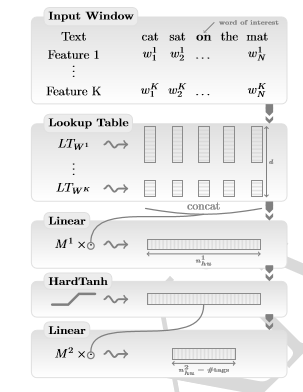
\includegraphics[width=\textwidth]{translations/f1.png}
\caption*{图一\ 单词方法的神经网络结构 \label{translation_f1}}
\end{center}
\end{figure}

\begin{figure}[!hbp]
\begin{center}
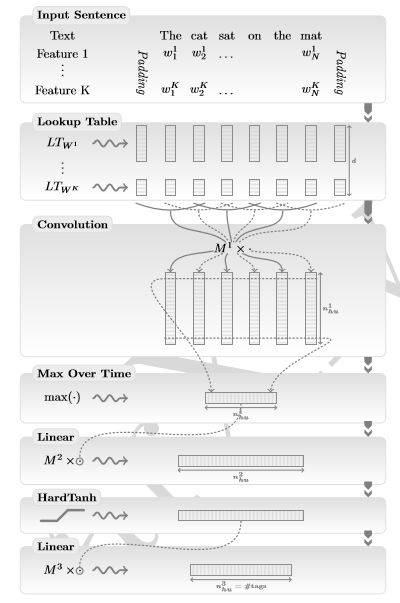
\includegraphics[width=\textwidth]{translations/f2.png}
\caption*{图二\ 句子方法的神经网络结构 \label{translation_f2}}
\end{center}
\end{figure}
\subsection*{3.1  将单词转化为特征向量}
我们结构的一个要点就是它在(几乎是)直接使用单词时也能发挥地很好。因此,对于我们的方法来说,学习到一个好的词语表达方式是非常重要的。为了保证效率,单词以在一个有限词典$D$中的序号的方式输入我们的结构。很明显,简单的序号并没有携带太多有用的信息。不过,网络的第一层通过查表操作将序号映射到一个特征向量上。在赋予了具体任务之后,每个单词的相关表示都能通过向后传播训练在对应的查找表格中找到。
正式来说,对于每个单词$w \in D$,通过查表层$LT_W(\cdot)$会赋予一个$d_{wrd}$维内部特征向量:
$$
LT_W(w) = {\left \langle W \right \rangle }^1_w
$$
此处,$W \in {\mathbb{R}}^{d_{wrd} \times |D|}$是需要被学习的参数矩阵,${\left \langle W \right \rangle}_w^1 \in {\mathbb{R}}^{d_{wrd}}$是W的第i列,而$d_{wrd}$是单词向量的长度(需要被用户选择的超参数)。
输入一句话或者长度为$T$的单词序列$[w]^T_1$,其中单词都存在于词典$D$中,则查表层会对序列中所有单词同样的操作,产生以下输出矩阵:
$$
LT_W([W]^T_1)=({\left \langle W \right \rangle }^1_{[w]_1}, {\left \langle W \right \rangle }^1_{[w]_2} ... {\left \langle W \right \rangle }^1_{[w]_r}) \eqno{1}
$$
该矩阵可以被应用于之后的神经网络层,我们在下文中将介绍。

\subsubsection*{3.1.1 拓展到任意离散特征}
当研究者们认为单词以外的特征对特定任务有帮助时,他们可能需要向神经网络输入这些特征。例如,在命名实体识别任务中,可能需要提供词语是否存在于地名词典中的特征。另外一个常见情况是需要引入一些基本的预处理,比如词干化或者需要处理大小写问题。在这种情况中,单词可能被三个离散特征代表:小写字母形式的词干,小写字母形式的结尾,首字母大写形式的词汇本身。
总的来说,我们可以假设词汇w被$K$个离散特征表示,此处$w \in D^1 \times ... \times D^K$, $D^k$代表第k个特征的词典。我们可以将每个特征与一个查找表$LT_{w^k}(\cdot)$关联起来,此处参数$W^k \in {\mathbb{R}}^{d_{wrd}^k \times |D_k|}$,$d_{wrd}^k \in \mathbb{N}$是用户定义的特征向量维度。对于单词w来说,特征向量维度为$d_{wrd}=\sum_k{d_{wrd}^k}$,由所有查找表的输出连接而成。
$$
LT_{W^1,...,W^K}(w) = \begin{pmatrix}
\\ LT_{W^1}(w_1)
\\. 
\\.
\\.
\\ LT_{W^K}(w_K)
\end{pmatrix} =
\begin{pmatrix}
\\ {\left \langle W^1 \right \rangle}^1_{w_1}
\\. 
\\.
\\.
\\ {\left \langle W^K \right \rangle}^1_{w_K}
\end{pmatrix}
$$
查找表的输出矩阵与(16)类似,但每个离散特征为其添加了额外的行:
$$
LT_{W^1,...,W^K}(|W|^T_1) = 
\begin{pmatrix}
\\{\left \langle W^1 \right \rangle}^1_{[W_1]_1} ... {\left \langle W^1 \right \rangle}^1_{[W_1]_T}
\\.
\\.
\\.
\\{\left \langle W^K \right \rangle}^1_{[W_K]_1} ... {\left \langle W^K \right \rangle}^1_{[W_K]_T}
\end{pmatrix} \eqno{2}
$$
这些查找表内的特征向量有效地学习了词典中词汇的特征。现在,我们可以将这些可训练的特征输入更深层次的可训练特征抽取流程,如此就可以表示词组,最终,表示整个句子。

\subsection*{3.2 从词汇特征向量中抽取高层次的特征向量}
查找表层产生的特征向量需要在后续神经网络层中被组合,以此决策句子中的每个单词的标签。为可变长序列中的元素产生标签(这里,句子是一个单词序列)是机器学习中的标准问题。我们提出了两种每次标注一个单词的通用方式:窗口方法和(基于卷积的)句子方法。

\subsubsection*{3.2.1 窗口方法}
窗口方法假设单词的标签主要依赖于它周围的单词。给定一个需要标注标签的单词,我们通常考虑从其周围$k_{sz}$(给定值,超参数)大小的单词窗口。所有在这个窗口内的单词都首先被传进查表层(16)或者(2),以产生大小为固定值$d_{wrd} \times k_{sz}$的单词特征矩阵。可以将该矩阵每列相连接,则此时该矩阵可以被视为$d_{wrd}k_{sz}$维的向量。正式地说,第一层网络输出的词窗口特征向量可以被写为:
$$
f_0^1 = {\left \langle LT_w({[w]_1^T})\right \rangle}_t^{d_{win}} = 
\begin{pmatrix}
\\{\left \langle W \right \rangle}^1_{{[w]}_{t-d_{win}/2}}
\\.
\\.
\\.
\\{\left \langle W \right \rangle}^1_{{[w]}_{t}}
\\.
\\.
\\.
\\{\left \langle W \right \rangle}^1_{{[w]}_{t+d_{win}/2}}
\end{pmatrix} \eqno{3}
$$

\paragraph*{线性层}
固定维度的向量$f_0^1$可以作为一层或多层标准神经网络层的输入,这些层为输入提供了几何映射:
$$
f_{\theta}^l=W_lf_{\theta}^{l-1} + b^l \eqno{4}
$$
这里$W^l \in {\mathbb{R}}^{n^{t}_{hu} \times n^{t-1}_{hu}},b^l \in {\mathbb{R}}^{n^{t}_{hu}}$都是需要被训练的参数,$n_{hu}^l$是超参数,代表第l层隐藏单元的数目。

\paragraph*{HardTanh层}
多层线性神经网络通常是被堆叠在一起的,使用非线性函数交织在一起,以抽取出高层的非线性的特征。如果没有引入非线性函数,那么我们的模型就将只是简单的线性模型。我们使用了双曲正切函数的“硬”版本作为非线性函数,它具有计算代价稍低的特点(与原本的双曲正切函数相比),同时能保持泛化表现不变(Collobert, 2004)。第l层在输入向量上应用HardTanh函数:
$$
{[f^l_{\theta}]}_i = HardTanh([f^{l-1}_{\theta}]),
$$
此处
$$
HardTanh(x) = \left\{\begin{matrix}
-1 & if\ x<-1 \\ 
x & if\ -1<=x<=1\\ 
1 & if\ x > 1 
\end{matrix} \right. \eqno{5}
$$

\paragraph*{打分}
最终,网络最后一层L的输出向量维数将会与相关任务的标签数目一致。每个输出之后都能被翻译为对应标签的分数(需要知道网络输入信息),这主要是因为我们仔细挑选了一个代价函数,该函数将在下面的章节介绍。

\paragraph*{备注1(边际效应)}
特征窗口没有很好地定义如何处理开头或者结尾处的单词。为了智慧地解决这个问题,我们使用了一个特殊的单词"PADDING"(填充)在句子首尾复制$d_{win}/2$次。这与使用"start"(开始)和"end"(结束)符号的方法本质上是一致的。

\subsection*{3.2.2 句子方法}
在实验结果分析章节我们将会发现仅仅只用窗口方法就能够解决大多数我们感兴趣的问题。但是,该方法难以解决语义角色标注问题。在该问题中某个词语的标签取决于在这个句子中位置比该词语更靠前的动词(更正式的说法是谓语)。如果该动词落在词语窗口之外,系统就不能够正确地分类该词语。在这种特殊情况下,分类这个词需要考虑整个句子。当使用神经网络时,我们可以自然地想到能够使用卷积神经网络解决该问题。该想法首先为Waibel等所提出(1989),在文献中被称作时延神经网络(Time Delay Neural Networks, TDNNs)。
我们会在接下来详细介绍卷积神经网络。它将整个句子连续输入,经过查表层(16),由卷积层在句中每个单词周围产生局部特征,将这些局部特征结合在一起可以生成全局特征向量,该向量可以输入标准的仿射层(4)。在语义角色标注的例子中,该操作在句子中的每个词语上,每个动词上执行。因此,在神经网络中标注希望纳入考虑的是哪个动词,希望进行标注的是哪个词语是非常重要的。为了这个目的,位置i上的词语会增加两个如3.1.1描述的特征,这些特征描述了两个相对距离$i-pos_v$和$i-pos_w$,此处被选择的动词在$pos_v$位置上,要被标注的单词在$pos_w$位置上。

\paragraph*{卷积层}
卷积层可以被视为窗口方法的一种泛化:给定一个由矩阵$f_{\theta}^{l - 1}$的若干列表示的序列(在查找表中(1)),(4)中的由矩阵转化为向量的操作在序列中连续的每个窗口内执行,用之前的记号,第l层输出第t列可以被计算为:
$$
{\left \langle {f_{\theta}^{l}}\right \rangle}^1_t = W^l{\left \langle {f_{\theta}^{l - 1}}\right \rangle}^{d_{win}}_t + b^l, \forall{t} \eqno{6}
$$
此处权重矩阵$W^l$在整个序列的所有窗口计算时保持不变。卷积层抽取给定序列每个窗口内的局部特征。为了输出给标准仿射层(4),若干卷积层通常被堆叠在一起以获取高层次的特征。在这种情况下,每层后面一定要使用非线性函数(5),否则整个卷积网络就相当于一层卷积网络。

\paragraph*{最大层}
输出(6)的大小取决于输入神经网络的句子的大小。被卷积神经网络抽取的局部特征向量需要被结合为全局特征向量,该向量需要有一个固定的,与句子长度无关的维数,以便于输入接下来的标准仿射层。传统卷积神经网络往往在序列(6)的时间t上使用计算平均值(计算时可能带有权重)或者最大值的方式完成这一点。(这里“时间”只代表其在句子中的位置,该术语来源于卷积神经网络的某些应用方式,例如语音数据,该数据为时间序列。)在我们的研究中,平均值没有很大意义。另外,通常来说大部分词语对给定词的语义角色标注都没有什么影响,因此,我们使用最大值方法,它迫使神经网络获取卷积层产生的最有用的局部特征(如图3所示)。设卷积层l-1的输出为矩阵$f_{\theta}^{l - 1}$,则最大层l的输出为向量$f_{\theta}^l$:
$$
{[f_{\theta}^l]}_i = \max_t{{f_{\theta}^{l-1}}_{i,t}} \ 1<=i<=n_{hu}^{t-1} \eqno{7}
$$
该定长全局特征随后可以输入标准仿射层(4)。如窗口方法一样,我们最终可以为每个可能的标签进行打分。

\subsection*{3.1  将单词转化为特征向量}

\begin{figure}[!hbp]
\begin{center}
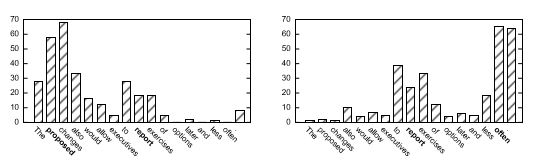
\includegraphics[width=\textwidth]{translations/f3.png}
\caption*{图三\ 每个词汇被最大层挑选的特征数量 \label{translation_f3}}
\end{center}
这张图片中我们考虑的是为了训练语义角色标注的图2中语句方法的神经网络。卷积神经网络产生的“局部”特征是每个单词300维,在使用过最大层后,我们得到了整个语句的300维特征。可以发现神经网络比较倾向与注意相关的动词(如"report")和词语(如"proposed"(左图),"often"(右图))
\end{figure}

\paragraph*{备注 2}
在卷积神经网络(6)中也有类似窗口方法(3)的边际效应,我们再次使用为句子填充特殊单词的方法解决这个问题。

\subsubsection*{3.2.3 标注方案}
如前述,神经网络输出层为当前任务的所有可能标签打分。在窗口方法中,这些标签对应于窗口正中心的词语,但在句子方法中,这些标签对应于网络输入中额外标记的单词。
词性标注任务实际上标注了每个词语的句法角色。剩下的三个任务的标签则主要依赖句子的一段。这三个任务通常用特殊的标注方案,如表3所示,以识别句子的段落。有些这样的方案已经被学者充分定义了(如IOB, IOE, IOBES,...),目前对于哪个方案更好还没有统一结论。最好的表现成果有时是通过结合通过不同标注方案训练的分类器获得的。
命名实体识别,分块和语义角色标注任务目前都使用了两种不同的标注方案。为了消除这个额外资源所带来的变化,我们决定所有任务中都使用最具有表达力的IOBES标注方案。举例来说,在分块任务中,我们用四种不同的标签来描述名词。标签"S-NP"用于描述只包含一个词语的名词短语。标签"B-NP","I-NP","E-NP"则分别描述具有多个词语的名词短语的第一个,中间和最后一个词语。还有一个额外的标签"O"用来表示这个单词不在分块之中。在测试时,这些标签又被转化为原本的IOB标签方案以便输入如2.5小节提到的标准性能评估阶段。

\begin{figure}[!hbp]
\begin{center}
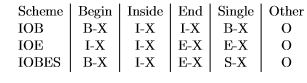
\includegraphics[width=\textwidth]{translations/f4.png}
\caption*{表三\ 不同的标注方案 \label{translation_f4}}
\end{center}
在分块中每个标注中存在"X"的单词都会根据位置(开头,中间,结尾)被标注上它的前缀。单独一个词语的分块也在输出中。不在已标注分块中的单词被标为"O"。IOB(和IOE)方案有一些变化,这里将不和其它带有"X"的分块邻接的分块前缀中"B"或者"E"替代为"I"。
\end{figure}

\subsection*{3.3 训练}
所有神经网络都通过使用随机梯度下降算法最大化训练数据的整体似然计算得到。如果我们令$\theta$为神经网络中所有可训练参数的代称,当用训练集$\mathbb{T}$训练时,我们希望最大化以下与$\theta$有关的似然:
$$
\theta \rightarrow \sum_{(x,y) \in \mathbb{T}}{\log{p(y|x, \theta)}} \eqno{8}
$$
这里x为一个训练词语窗口或者句子以及其相关的特征,y代表与之相关的正确标签。概率$p(\cdot)$由神经网络的输出与标签计算而来。我们会在接下来的部分看到如何将神经网络的输出转化为概率。

\subsubsection*{3.3.1 单词层级的似然对数值}
在这种方法中,句子中的每个单词都被认为是独立的。给定输入样例为x,则参数为$\theta$的神经网络输出的对于第i个标签的分数为${[f_{\theta}(x)]}_i$。为了简化该记号,我们先去除x的影响,只考虑${[f_{\theta}]}_i$。则分数可以通过在所有可用标签上执行softmax操作而被转化为标签的条件概率$p(i|x,\theta)$:
$$
p(i|x, \theta) = \frac{e^{{[f_{\theta}]}_i}}{\sum_i{e^{{[f_{\theta}]}_i}}} \eqno{9}
$$
定义操作log-add为:
$$
\mathop{logadd}_iz_i = log(\sum_i e^{zi}) \eqno{11}
$$
如此,我们就能够像这样表达某个训练样本$(x,y)$的似然对数值:
$$
\log p(y|x, \theta) = {[f_{\theta}]}_y - \mathop{logadd}_j{[f_{\theta}]}_j \eqno{11}
$$
该训练公式通常又被视为交叉熵,其被广泛地应用在分类问题中。在我们的例子中它也许不是最好的,因为通常句子中的某个词语的标签和周围单词的标签有某种联系。在接下来的章节我们将介绍另一个神经网络常用的计算方法,这种方法注重一个句子中被预测出的标签之间的依赖关系。

\subsubsection*{3.3.2 语句层级的似然对数值}
在类似于分块,命名实体识别,语义角色标注的任务中,我们知道在语句中的标签彼此存在依赖关系:有些标签主要与分块有关,有些则不应该被另外一些标签影响。我们考虑了一种将句子结构纳入考虑的训练方案:当给定神经网络对某个句子中所有单词的标签预测,且给定标签转移的分数,我们希望能鼓励一些标签转化的路径生成,同时抑制另外一些路径。
考虑神经网络的分数矩阵$f_{\theta}({[x]}_1^{\mathbb{T}})$,像前一个章节的方法一样,为了简化符号,我们暂时不考虑输入${[x]}_1^{\mathbb{T}}$的影响。则${[f_{\theta}]}_{i,t}$为在语句${[x]}_1^{\mathbb{T}}$对应第i个单词,第i个标签,且参数为${\theta}$的分数输出。
在此我们提出转移分数这个概念,${[A]}_{i,j}$代表在连续的单词中从标签i转移到标签j的分数。${[A]}_{i,0}$则代表从第i个标签开始的分数。由于转移分数矩阵与${\theta}$类似,也是要被训练的参数之一,我们定义$\tilde{\theta} = \theta \cup {\{{[A]}_{i,j}\ \forall i, j\}}$。则语句${[x]}_1^{\mathbb{T}}$沿着路径${[i]}_1^{\mathbb{T}}$的分数可由转移分数和网络输出分数之和给出:
$$
s({[x]}_1^{\mathbb{T}}, {[i]}_1^{\mathbb{T}}, \tilde{\theta}) = \sum^{\mathbb{T}}_{t=1}({[A]}_{{[i ]}_{t - 1}, {[i ]}_{t}} + {[f_{\theta}]}_{{[i]_t}, t}) \eqno{12}
$$
与词语层级的似然值(11)很相近,在词语层级我们使用softmax(9)归一化所有标签,在语句层级我们也使用softmax归一化所有可能的标签路径${[j]}^{\mathbb{T}}_1$,然后我们将结果比值转化为标签路径的条件概率。在对数操作后,真正的路径${[y]}_1^{\mathbb{T}}$的条件概率为:
$$
\log{p({[y]}_1^{\mathbb{T}}| {[x]}_1^{\mathbb{T}}, \tilde{\theta})} = s({[x]}_1^{\mathbb{T}}, {[i]}_1^{\mathbb{T}}, \tilde{\theta}) - \mathop{logadd}_{\forall {[j]}_1^{\mathbb{T}}}\ {s({[x]}_1^{\mathbb{T}}, {[i]}_1^{\mathbb{T}}, \tilde{\theta})} \eqno{13}
$$  
由于logadd操作(11)中的短语个数与标签个数相同,所以在(13)中它随句子的长度指数性增长。幸运的是,利用在半环($\mathbb{R} \cup \{-{\infty}\}, logadd, +$)上的结合律和分布律,我们可以重复以下关于t的标准迭代在线性时间计算出结果:
$$
\begin{matrix}
{\delta}_t(k) & \triangleq \mathop{logadd}_{{[j]}^t_1 \cap {[j]}_t = k} s({[x]}_1^{t}, {[i]}_1^{t}, \tilde{\theta}) \\
& = \mathop{logadd}_i{\ \mathop{logadd}_{{[j]}^t_1 \cap {[j]}_{t-1} = i \cap {[j]_t = k}}} s({[x]}_1^{t}, {[j]}_1^{t-1}, \tilde{\theta}) + {[A]}_{{[j]}_{t-1,k}} + {[f_{\theta}]}_{k, t}\\
& = \mathop{logadd}_{i}{\  {\delta}_{t - 1}(i)} + {[A]}_{i,k} + {[f_{\theta}]}_{k,t}\\
& = {[f_{\theta}]}_{k,t} + \mathop{logadd}_{i}{\  ({\delta}_{t - 1}(i) + {[A]}_{i, k})}, \forall k, 
\end{matrix} \eqno{14}
$$
终止条件为:
$$
\mathop{logadd}_{\forall {[j]}_1^{\mathbb{T}}} s({[x]}_1^{\mathbb{T}}, {[i]}_1^{\mathbb{T}}, \tilde{\theta}) = \mathop{logadd}_i{\ \delta_{\mathbb{T}}(i)} \eqno{15}
$$
我们现在可以在所有训练样本对$({[x]}_1^{\mathbb{T}}, {[y]}_1^{\mathbb{T}})$对(8)中最大化似然值(13)。
在推测阶段,对于给定的语句${[x]}_1^{\mathbb{T}}$,我们需要找到最好的标签路径,以最小化语句分值(12),也就是说我们必须找到:
$$
\mathop{argmax}_{{[y]}_1^{\mathbb{T}}}s({[x]}_1^{\mathbb{T}}, {[i]}_1^{\mathbb{T}}, \tilde{\theta})\eqno{16}
$$
此时使用Viterbi算法是非常自然的选择,因为它相当于每步都在迭代(14)和(15),不过在Viterbi算法中logadd被max所代替,最后通过每个max找回最优路径。


\newpage
\section*{外文译文原文}
\begin{center}
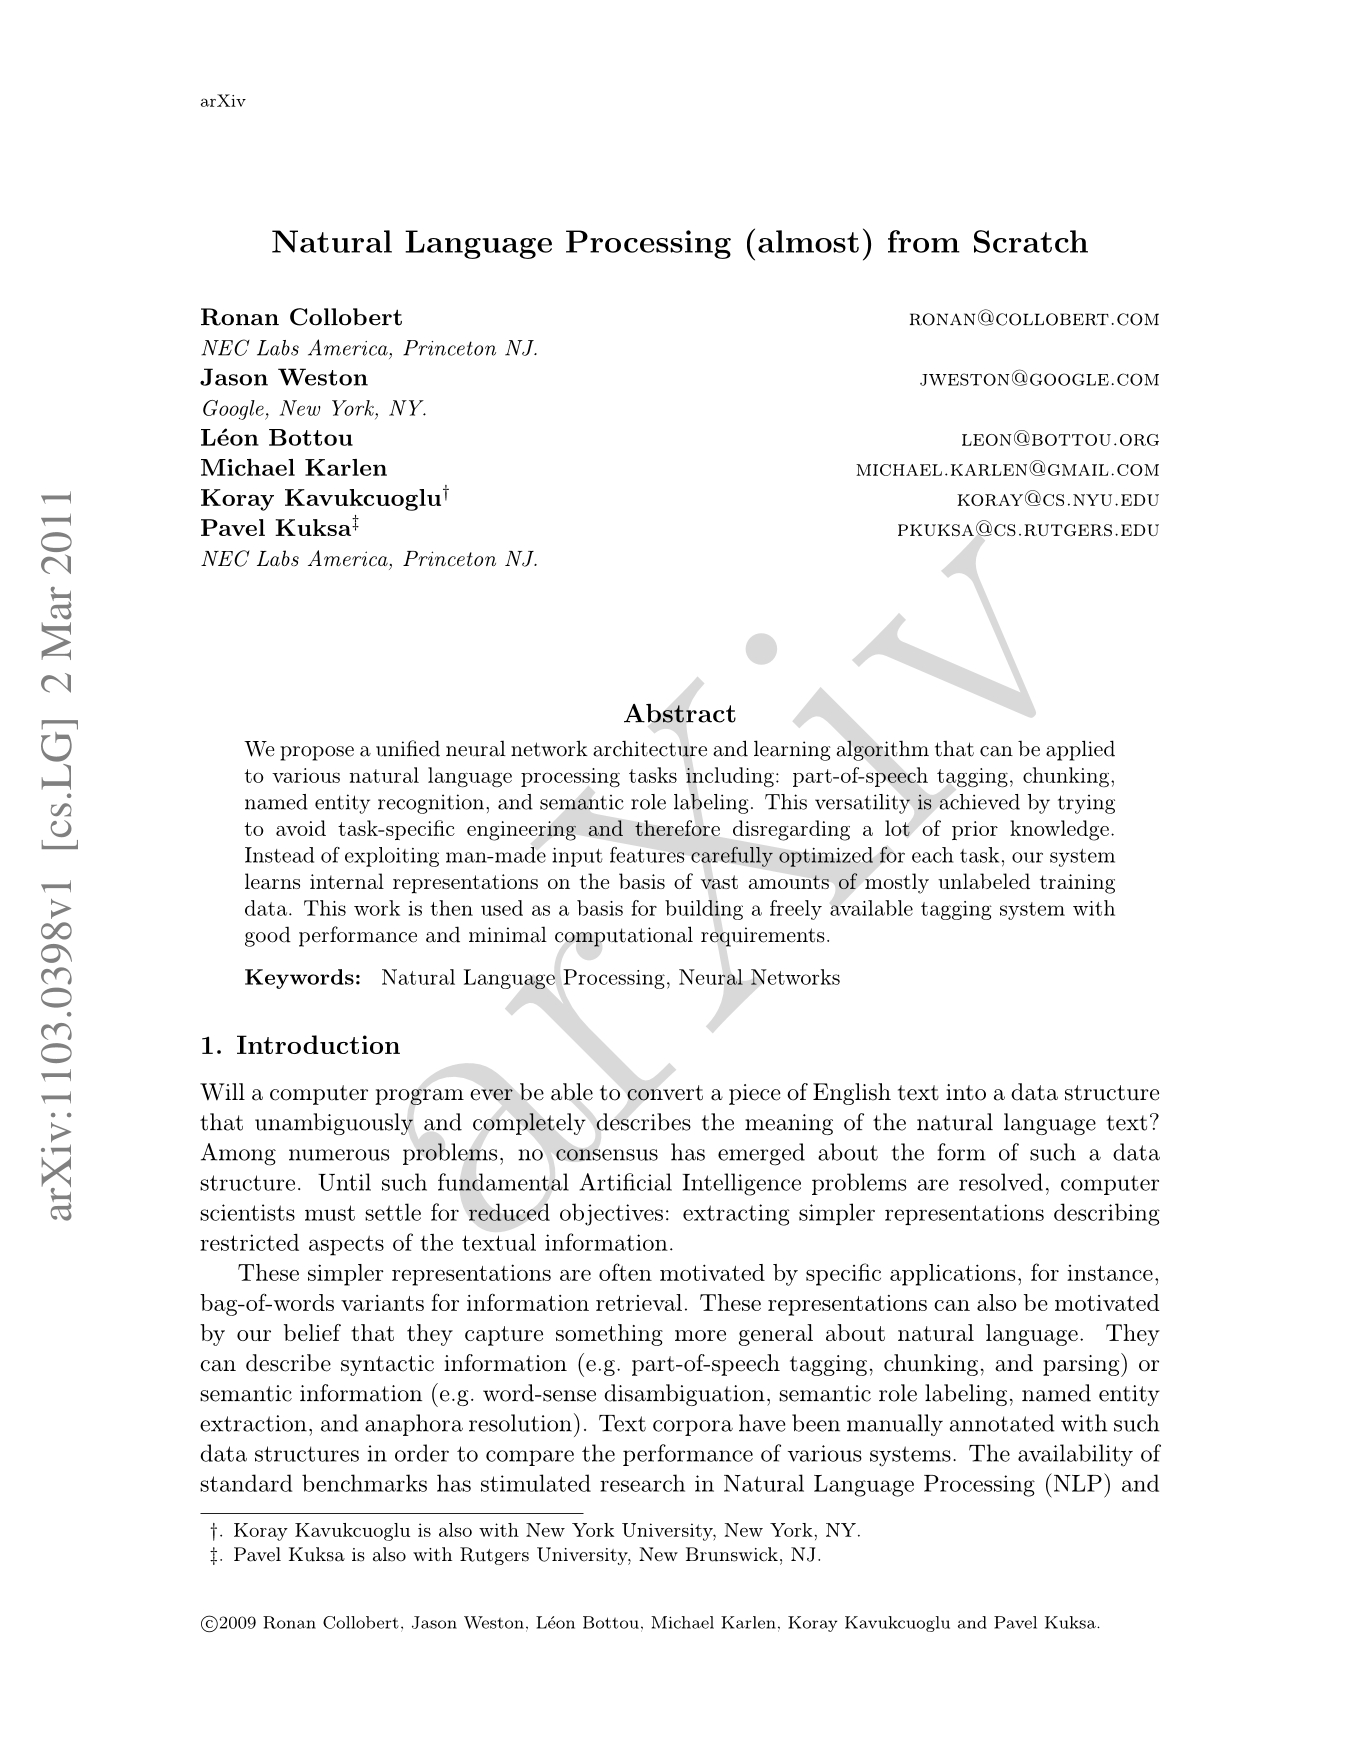
\includegraphics[width=\textwidth]{translations/collobert_2011-1.jpg}
\end{center}
\begin{center}
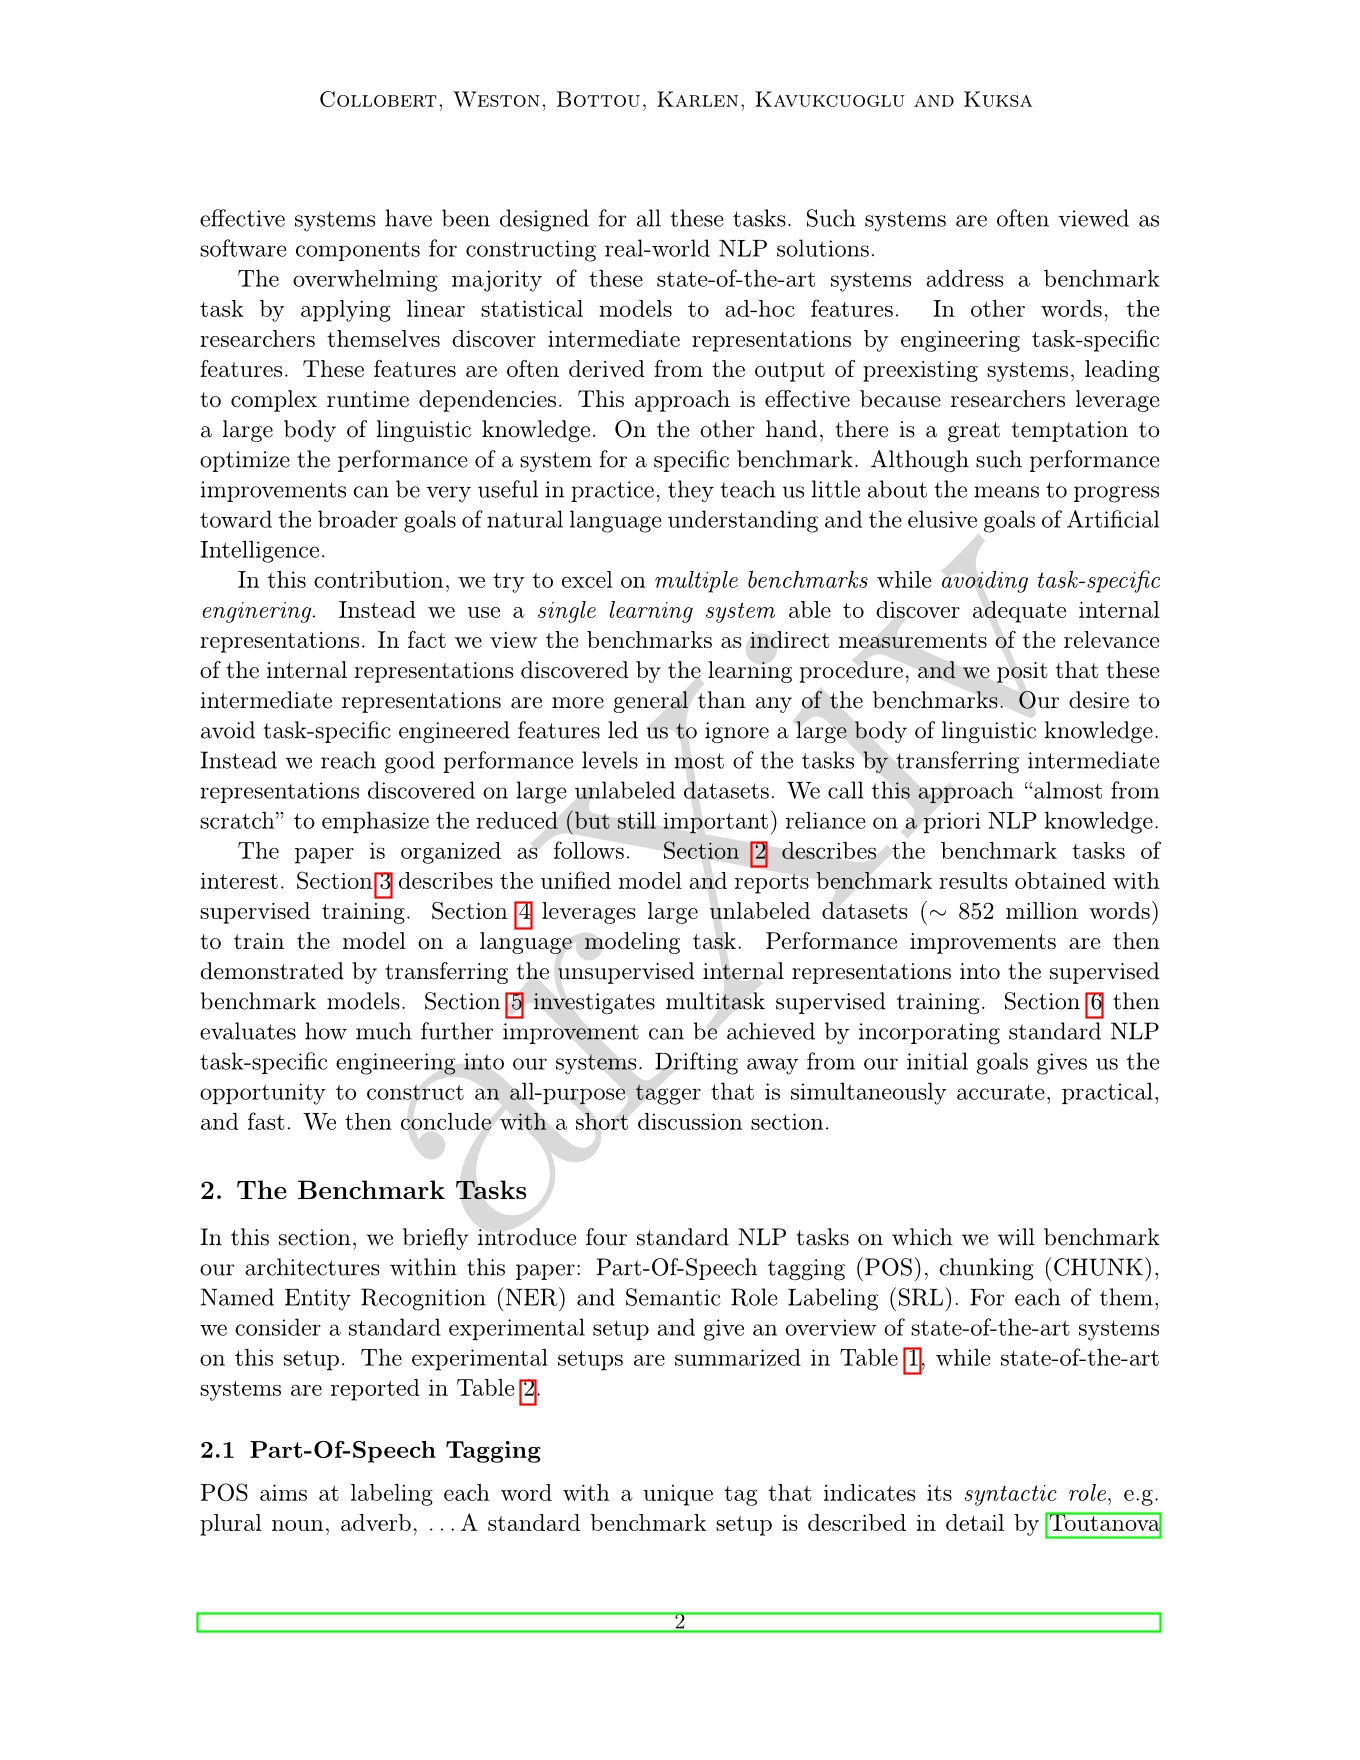
\includegraphics[width=\textwidth]{translations/collobert_2011-2.jpg}
\end{center}
\begin{center}
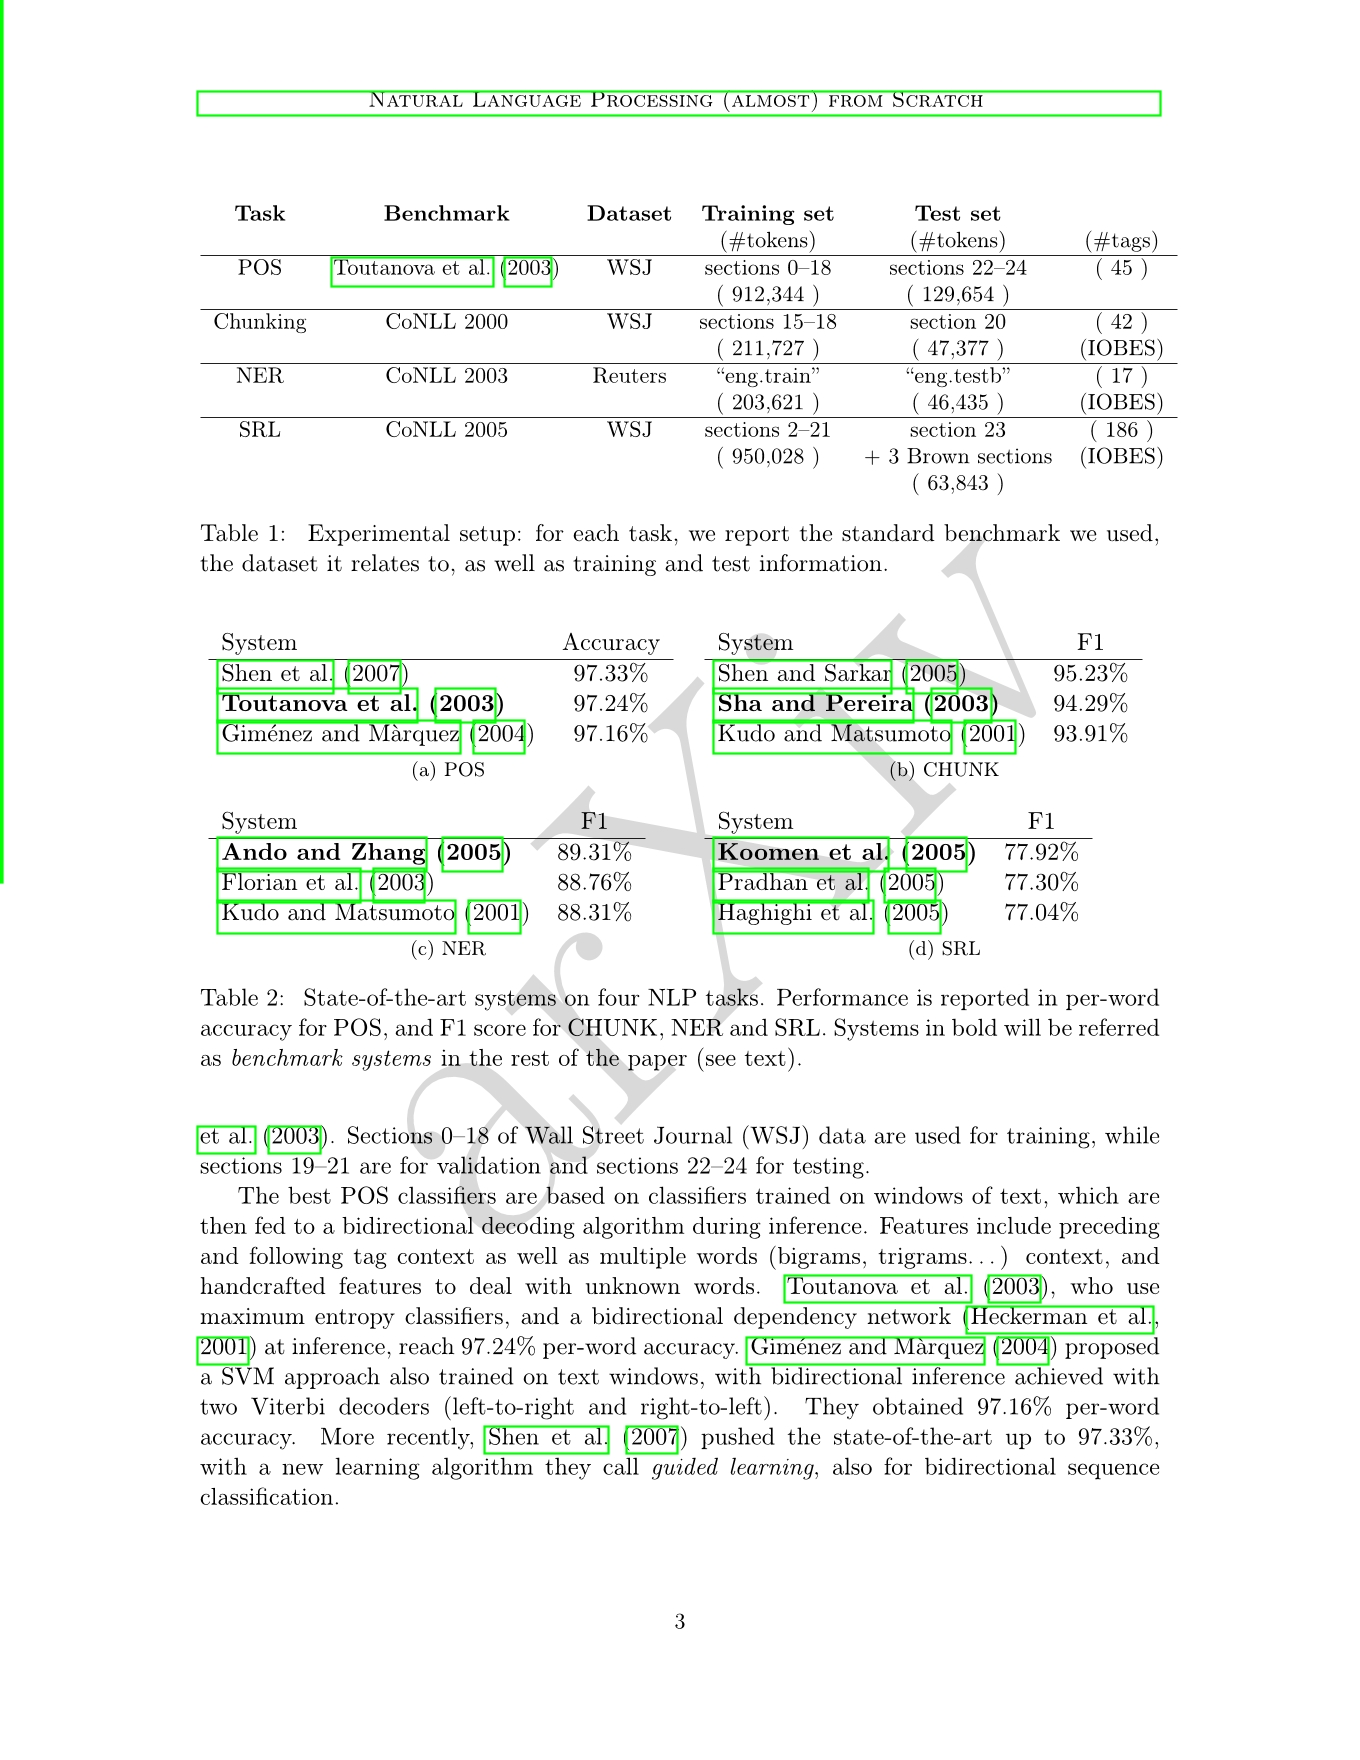
\includegraphics[width=\textwidth]{translations/collobert_2011-3.jpg}
\end{center}
\begin{center}
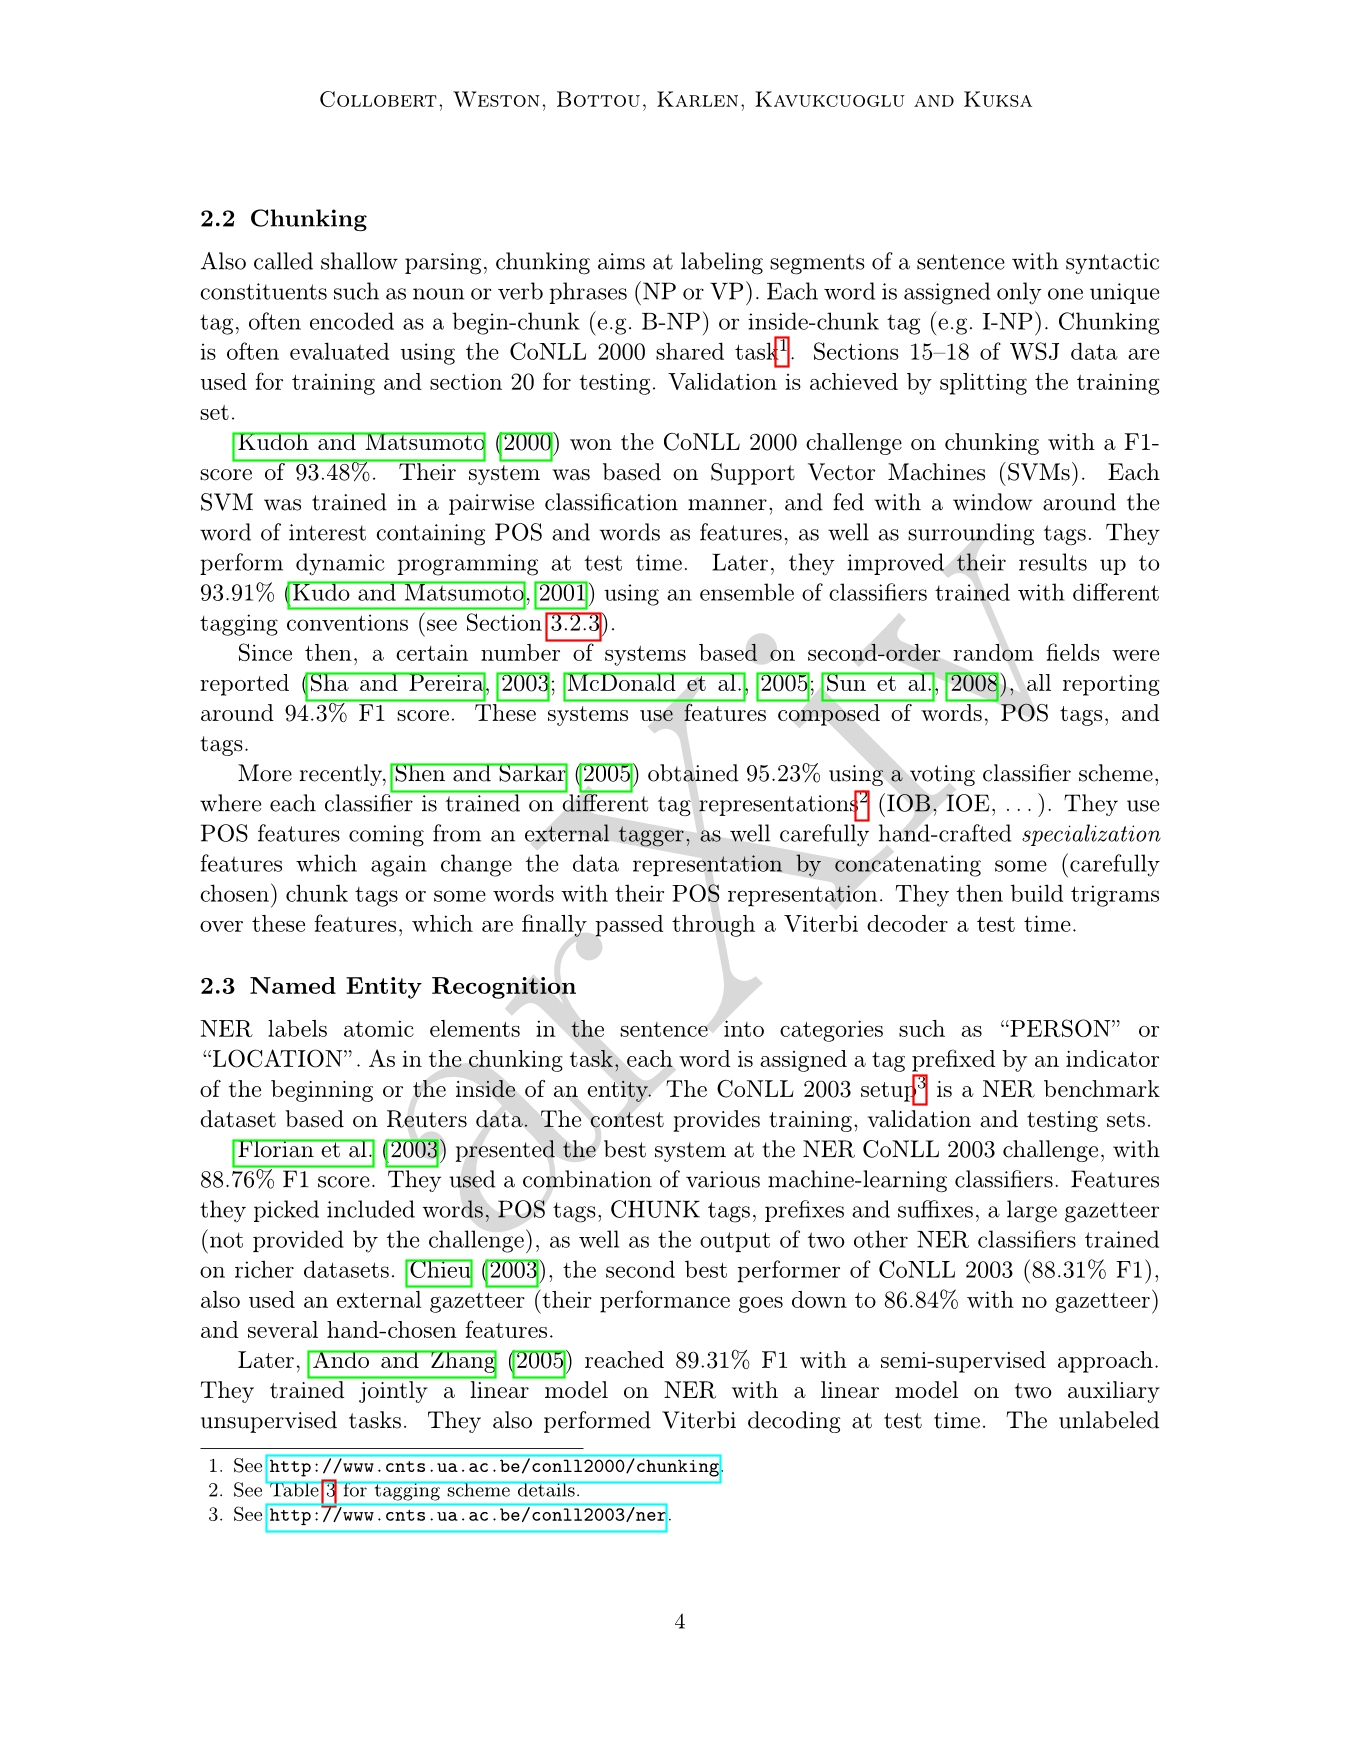
\includegraphics[width=\textwidth]{translations/collobert_2011-4.jpg}
\end{center}
\begin{center}
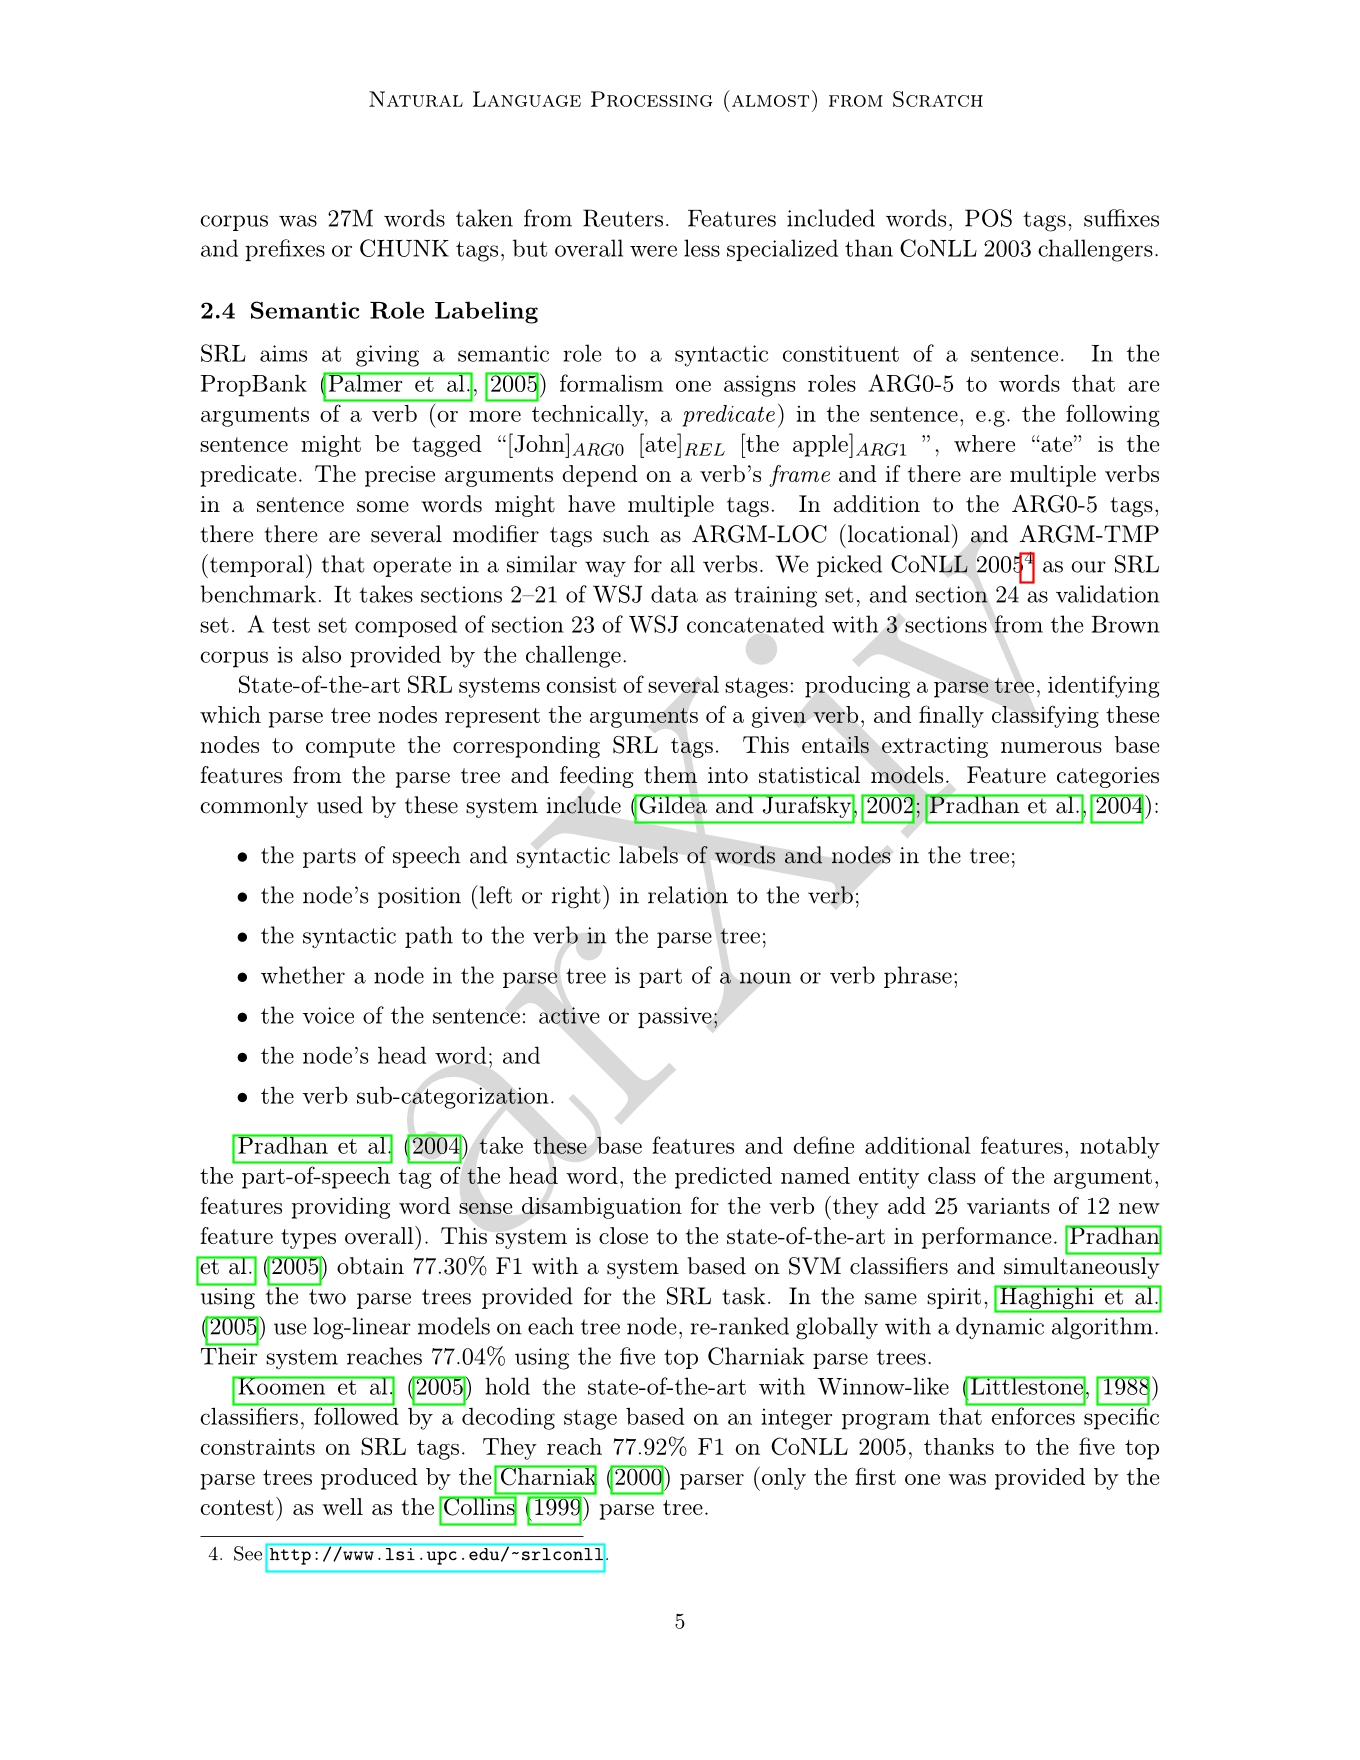
\includegraphics[width=\textwidth]{translations/collobert_2011-5.jpg}
\end{center}
\begin{center}
\includegraphics[width=\textwidth]{translations/collobert_2011-6.jpg}
\end{center}
\begin{center}
\includegraphics[width=\textwidth]{translations/collobert_2011-7.jpg}
\end{center}
\begin{center}
\includegraphics[width=\textwidth]{translations/collobert_2011-8.jpg}
\end{center}
\begin{center}
\includegraphics[width=\textwidth]{translations/collobert_2011-9.jpg}
\end{center}
\begin{center}
\includegraphics[width=\textwidth]{translations/collobert_2011-10.jpg}
\end{center}
\begin{center}
\includegraphics[width=\textwidth]{translations/collobert_2011-11.jpg}
\end{center}
\begin{center}
\includegraphics[width=\textwidth]{translations/collobert_2011-12.jpg}
\end{center}
\begin{center}
\includegraphics[width=\textwidth]{translations/collobert_2011-13.jpg}
\end{center}
\begin{center}
\includegraphics[width=\textwidth]{translations/collobert_2011-14.jpg}
\end{center}
\begin{center}
\includegraphics[width=\textwidth]{translations/collobert_2011-15.jpg}
\end{center}
\begin{center}
\includegraphics[width=\textwidth]{translations/collobert_2011-16.jpg}
\end{center}
\begin{center}
\includegraphics[width=\textwidth]{translations/collobert_2011-17.jpg}
\end{center}
\begin{center}
\includegraphics[width=\textwidth]{translations/collobert_2011-18.jpg}
\end{center}
\begin{center}
\includegraphics[width=\textwidth]{translations/collobert_2011-19.jpg}
\end{center}
\begin{center}
\includegraphics[width=\textwidth]{translations/collobert_2011-20.jpg}
\end{center}
\begin{center}
\includegraphics[width=\textwidth]{translations/collobert_2011-21.jpg}
\end{center}
\begin{center}
\includegraphics[width=\textwidth]{translations/collobert_2011-22.jpg}
\end{center}
\begin{center}
\includegraphics[width=\textwidth]{translations/collobert_2011-23.jpg}
\end{center}
\begin{center}
\includegraphics[width=\textwidth]{translations/collobert_2011-24.jpg}
\end{center}
\begin{center}
\includegraphics[width=\textwidth]{translations/collobert_2011-25.jpg}
\end{center}
\begin{center}
\includegraphics[width=\textwidth]{translations/collobert_2011-26.jpg}
\end{center}
\begin{center}
\includegraphics[width=\textwidth]{translations/collobert_2011-27.jpg}
\end{center}
\begin{center}
\includegraphics[width=\textwidth]{translations/collobert_2011-28.jpg}
\end{center}
\begin{center}
\includegraphics[width=\textwidth]{translations/collobert_2011-29.jpg}
\end{center}
\begin{center}
\includegraphics[width=\textwidth]{translations/collobert_2011-30.jpg}
\end{center}
\begin{center}
\includegraphics[width=\textwidth]{translations/collobert_2011-31.jpg}
\end{center}
\begin{center}
\includegraphics[width=\textwidth]{translations/collobert_2011-32.jpg}
\end{center}
\begin{center}
\includegraphics[width=\textwidth]{translations/collobert_2011-33.jpg}
\end{center}
\begin{center}
\includegraphics[width=\textwidth]{translations/collobert_2011-34.jpg}
\end{center}
\begin{center}
\includegraphics[width=\textwidth]{translations/collobert_2011-35.jpg}
\end{center}
\begin{center}
\includegraphics[width=\textwidth]{translations/collobert_2011-36.jpg}
\end{center}
\begin{center}
\includegraphics[width=\textwidth]{translations/collobert_2011-37.jpg}
\end{center}
\begin{center}
\includegraphics[width=\textwidth]{translations/collobert_2011-38.jpg}
\end{center}
\begin{center}
\includegraphics[width=\textwidth]{translations/collobert_2011-39.jpg}
\end{center}
\begin{center}
\includegraphics[width=\textwidth]{translations/collobert_2011-40.jpg}
\end{center}
\begin{center}
\includegraphics[width=\textwidth]{translations/collobert_2011-41.jpg}
\end{center}
\begin{center}
\includegraphics[width=\textwidth]{translations/collobert_2011-42.jpg}
\end{center}
\begin{center}
\includegraphics[width=\textwidth]{translations/collobert_2011-43.jpg}
\end{center}
\begin{center}
\includegraphics[width=\textwidth]{translations/collobert_2011-44.jpg}
\end{center}
\begin{center}
\includegraphics[width=\textwidth]{translations/collobert_2011-45.jpg}
\end{center}
\begin{center}
\includegraphics[width=\textwidth]{translations/collobert_2011-46.jpg}
\end{center}
\begin{center}
\includegraphics[width=\textwidth]{translations/collobert_2011-47.jpg}
\end{center}

\end{document}

